%%%%%%%%%%%%%%%%%%%%%%%%%%%%%%%%%%%%%%%%%
% Masters/Doctoral Thesis 
% LaTeX Template
% Version 2.5 (27/8/17)
%
% This template was downloaded from:
% http://www.LaTeXTemplates.com
%
% Version 2.x major modifications by:
% Vel (vel@latextemplates.com)
%
% This template is based on a template by:
% Steve Gunn (http://users.ecs.soton.ac.uk/srg/softwaretools/document/templates/)
% Sunil Patel (http://www.sunilpatel.co.uk/thesis-template/)
%
% Template license:
% CC BY-NC-SA 3.0 (http://creativecommons.org/licenses/by-nc-sa/3.0/)
%
%%%%%%%%%%%%%%%%%%%%%%%%%%%%%%%%%%%%%%%%%

%----------------------------------------------------------------------------------------
%	PACKAGES AND OTHER DOCUMENT CONFIGURATIONS
%----------------------------------------------------------------------------------------

\documentclass[
% The default document font size, options: 10pt, 11pt, 12pt
11pt, 
% Two side (alternating margins) for binding by default, uncomment to switch to one side
oneside,
% ngerman for German
english,
% Single line spacing, alternatives: singlespacing, onehalfspacing or doublespacing
onehalfspacing,
% Uncomment to enable draft mode (no pictures, no links, overfull hboxes indicated)
%draft,
% If the document is nolistspacing, onehalfspacing or doublespacing, uncomment this to set spacing in lists to single
onehalfspacing,
% Uncomment to add the list of figures/tables/etc to the table of contents
%liststotoc,
% Uncomment to add the main table of contents to the table of contents
%toctotoc,
% Uncomment to add space between paragraphs
parskip,
% Uncomment to not load the hyperref package
%nohyperref,
% Uncomment to get a line under the header
headsepline,
% Uncomment to place the chapter title next to the number on one line
%chapterinoneline,
% Uncomment to change the layout of the declaration, abstract and acknowledgements pages to match the default layout
%consistentlayout,
% The class file specifying the document structure
]{MastersDoctoralThesis}

% Required for inputting international characters
\usepackage[utf8]{inputenc}

% Output font encoding for international characters
\usepackage[T1]{fontenc}
\usepackage{textcomp} % support the degree symbol

% Use the Palatino font by default
\usepackage{mathpazo}

% Use tu justify paragraphs
\usepackage{ragged2e}

% Use the bibtex backend with the authoryear citation style (which resembles APA)
\usepackage[backend=biber,natbib=true]{biblatex}
% MLA, APA, or IEEE? - https://www.overleaf.com/learn/latex/Biblatex_citation_styles
%\usepackage[style=apa, backend=biber]{biblatex}

% The filename of the bibliography
\addbibresource{mainBiblio.bib}

% Required to generate language-dependent quotes in the bibliography
\usepackage[autostyle=true]{csquotes}

% to set default colours
\usepackage{xcolor}
\definecolor{mygray}{gray}{0.5}

% for gantt charts
\usepackage{tikz}
\usepackage{gantt}

% to rotate pages in landscape
\usepackage{lscape}

% equation arrows with text
\usepackage{amsmath}

% insert degree celsius symbol
\usepackage{textcomp}

% include other pdf pages
\usepackage{pdfpages}

% stop all hyphenation
%\raggedright
\sloppy
\usepackage[none]{hyphenat}

%----------------------------------------------------------------------------------------
%	MARGIN SETTINGS
%----------------------------------------------------------------------------------------

\geometry{
	paper=a4paper,      % Change to letterpaper for US letter
	inner=2.5cm,        % Inner margin
	outer=3.8cm,        % Outer margin
	bindingoffset=.5cm, % Binding offset
	top=1.5cm,          % Top margin
	bottom=1.5cm,       % Bottom margin
	%showframe,         % Uncomment to show how the type block is set on the page
}

%----------------------------------------------------------------------------------------
%	THESIS INFORMATION
%----------------------------------------------------------------------------------------

% Your thesis title, this is used in the title and abstract, print it elsewhere with \ttitle
\thesistitle{Fabrication of Graphitic-Carbon Suspended Nanowires Through Mechano-Near-Field Electrospinning of Photocrosslinkable Polymers}

% Your supervisor's name, this is used in the title page, print it elsewhere with \supname and \cosupname
\supervisor{Dr. Héctor Alán \textsc{Aguirre} Soto}
\cosupervisor{Dra. Dora Iliana \textsc{Medina} Medina}

% Your examiner's name, this is not currently used anywhere in the template, print it elsewhere with \examname
\examiner{}

% Your degree name, this is used in the title page and abstract, print it elsewhere with \degreename
\degree{Master of Science in Nanotechnology (MNT)}

% Your name, this is used in the title page and abstract, print it elsewhere with \authorname
\author{Antonio Osamu \textsc{Katagiri} Tanaka}

% Your address, this is not currently used anywhere in the template, print it elsewhere with \addressname
\addresses{Estado de México, Atizapan de Zaragoza}

% Your subject area, this is not currently used anywhere in the template, print it elsewhere with \subjectname
\subject{Nanotechnology}

% Keywords for your thesis, this is not currently used anywhere in the template, print it elsewhere with \keywordnames
\keywords{nanotechnology, carbon, nano-wires, electrospinning, NFES}

% Your university's name and URL, this is used in the title page and abstract, print it elsewhere with \univname
\university{\href{https://tec.mx/}{Instituto Tecnonólogico y de Estudios Superiores de Monterrey}}

% Your university's campus name and URL, this is used in the title page and abstract, print it elsewhere with \campusname
\campus{\href{https://tec.mx/}{Campus Estado de México}}

% Your department's name and URL, this is used in the title page and abstract, print it elsewhere with \deptname
\department{\href{https://tec.mx/}{School of Engineering and Sciences}}

% Your research group's name and URL, this is used in the title page, print it elsewhere with \groupname
\group{\href{https://www.medinadora.com/people}{ITESM \campusname}}

% Your faculty's name and URL, this is used in the title page and abstract, print it elsewhere with \facname
\faculty{\href{https://samp.itesm.mx/Programas/VistaPrograma?clave=MNT16&modoVista=Default&idioma=ES&cols=0}{Faculty: Nanotechnology}}

\AtBeginDocument{
\hypersetup{pdftitle=\ttitle}          % Set the PDF's title to your title
\hypersetup{pdfauthor=\authorname}     % Set the PDF's author to your name
\hypersetup{pdfkeywords=\keywordnames} % Set the PDF's keywords to your keywords
}

\begin{document}

% Use roman page numbering style (i, ii, iii, iv...) for the pre-content pages
\frontmatter

% Default to the plain heading style until the thesis style is called for the body content
\pagestyle{plain} 

%----------------------------------------------------------------------------------------
%	TITLE/COVER PAGE
%----------------------------------------------------------------------------------------

\begin{titlepage}
\begin{center}

\vspace*{.06\textheight}
{\scshape\LARGE \univname\par} % University name

\begin{center}

\includegraphics[width=0.15\textwidth]{./Figures/uniLogo.png}
\end{center}

\vspace{0.5cm}
\textsc{\Large Masters Thesis Proposal}\\[0.5cm]      % Thesis type

\HRule \\%[0.5cm]                           % Horizontal line
{\huge \bfseries \ttitle\par}\vspace{0.0cm} % Thesis title
\HRule \\[0.5cm]                            % Horizontal line
 
\begin{minipage}[t]{0.4\textwidth}
\begin{flushleft} \large
\emph{Author:}\\

% Author name - remove the \href bracket to remove the link
\href{https://linkedin.com/in/osamu-katagiri-84b2b940/}{\authorname}
%\authorname
\end{flushleft}
\end{minipage}
\begin{minipage}[t]{0.4\textwidth}
\begin{flushright} \large
\emph{Principal Advisor:} \\
% Supervisor name - remove the \href bracket to remove the link
%\href{http://www.doramedina.com}{\supname}
\supname

\bigskip

\emph{Co-advisor and\\Director of Program:} \\
% Supervisor name - remove the \href bracket to remove the link
\href{https://www.medinadora.com/}{\cosupname}
%\cosupname
\end{flushright}
\end{minipage}\\[0.5cm]
 
\vfill

\large \textit{A thesis proposal submitted in fulfillment of the requirements\\ for the degree of
% University requirement text
\degreename}\\[0.25cm]
\textit{in}\\[0.25cm]
% Research group name and department name
\groupname\\\deptname\\[1cm]
 
\vfill

% Address and Date
{\addressname \text{, } \large \today}\\[4cm]
% University/department logo - uncomment to place it
%
\includegraphics{./Figures/uniLogo.png}
 
\vfill
\end{center}
\end{titlepage}

%----------------------------------------------------------------------------------------
%	COMMITTEE'S PAGE
%----------------------------------------------------------------------------------------

%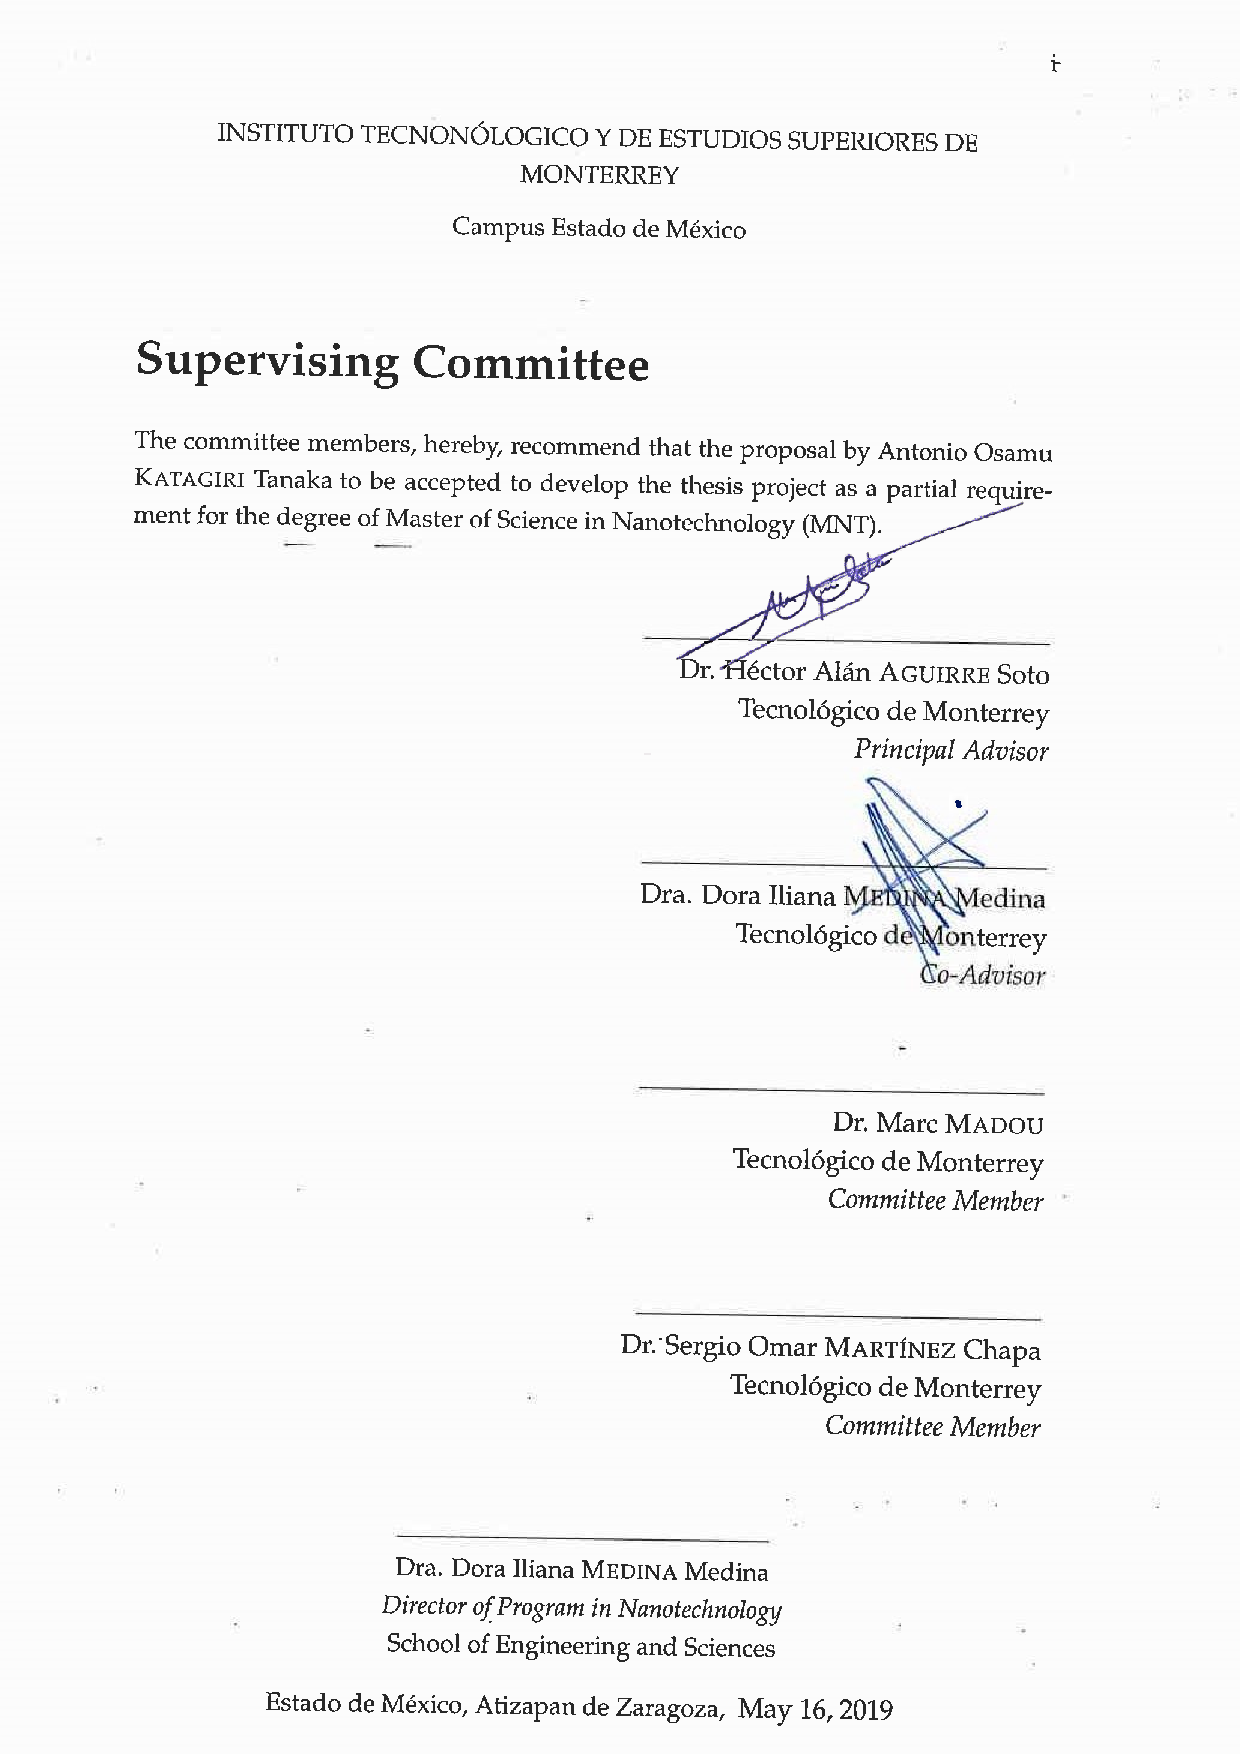
\includepdf[page=-]{./pdf/AlanDoraSigns}

\begin{committee}
\addchaptertocentry{\supervisingcommittee} % Add the the supervising committee to the table of contents
The committee members, hereby, recommend that the proposal by \authorname \text{ }to be accepted to develop the thesis project as a partial requirement for the degree of \degreename.

\begin{flushright} \large

\bigskip
\bigskip
\medskip

\noindent \rule[0.0em]{15em}{0.5pt}\\ % This prints a line for the signature
%\href{http://www.alanaguirre.com}{\supname}
\supname\\
Tecnológico de Monterrey\\
\emph{Principal Advisor}

\bigskip
\bigskip
\medskip

\noindent \rule[0.0em]{15em}{0.5pt}\\ % This prints a line for the signature
%\href{http://www.alanaguirre.com}{\supname}
\cosupname\\
Tecnológico de Monterrey\\
\emph{Co-Advisor}

\bigskip
\bigskip
\medskip

\noindent \rule[0.0em]{15em}{0.5pt}\\ % This prints a line for the signature
%\href{http://www.alanaguirre.com}{\supname}
Dr. Marc \textsc{Madou}\\
Tecnológico de Monterrey\\
\emph{Committee Member}

\bigskip
\bigskip
\medskip

\noindent \rule[0.0em]{15em}{0.5pt}\\ % This prints a line for the signature
%\href{http://www.alanaguirre.com}{\supname}
Dr. Sergio Omar \textsc{Martínez} Chapa\\
Tecnológico de Monterrey\\
\emph{Committee Member}

\end{flushright}

\vfill

\begin{center}

\bigskip
\bigskip
\medskip

\noindent \rule[0.0em]{15em}{0.5pt}\\ % This prints a line for the signature
\cosupname \\
\emph{Director of Program in Nanotechnology}\\
School of Engineering and Sciences\\
%\href{http://www.doramedina.com}{\supname}

\bigskip
{\addressname \text{, } \large \today}\\[0cm]

\end{center}
\end{committee}

\cleardoublepage

%----------------------------------------------------------------------------------------
%	DECLARATION PAGE
%----------------------------------------------------------------------------------------

\begin{declaration}
\addchaptertocentry{\authorshipname} % Add the declaration to the table of contents
\noindent I, \authorname, declare that this thesis titled, \enquote{\ttitle} and the work presented in it are my own. I confirm that:

\begin{itemize} 
\item This work was done wholly or mainly while in candidature for a research degree at this University.
\item Where any part of this thesis has previously been submitted for a degree or any other qualification at this University or any other institution, this has been clearly stated.
\item Where I have consulted the published work of others, this is always clearly attributed.
\item Where I have quoted from the work of others, the source is always given. With the exception of such quotations, this thesis is entirely my own work.
\item I have acknowledged all main sources of help.
\item Where the thesis is based on work done by myself jointly with others, I have made clear exactly what was done by others and what I have contributed myself.\\
\end{itemize}
 
\noindent Signed:\\
\rule[0.5em]{25em}{0.5pt} % This prints a line for the signature
 
\noindent Date:\\
\rule[0.5em]{25em}{0.5pt} % This prints a line to write the date
\end{declaration}

\cleardoublepage

%----------------------------------------------------------------------------------------
%	QUOTATION PAGE
%----------------------------------------------------------------------------------------

\vspace*{0.2\textheight}

\begin{center}
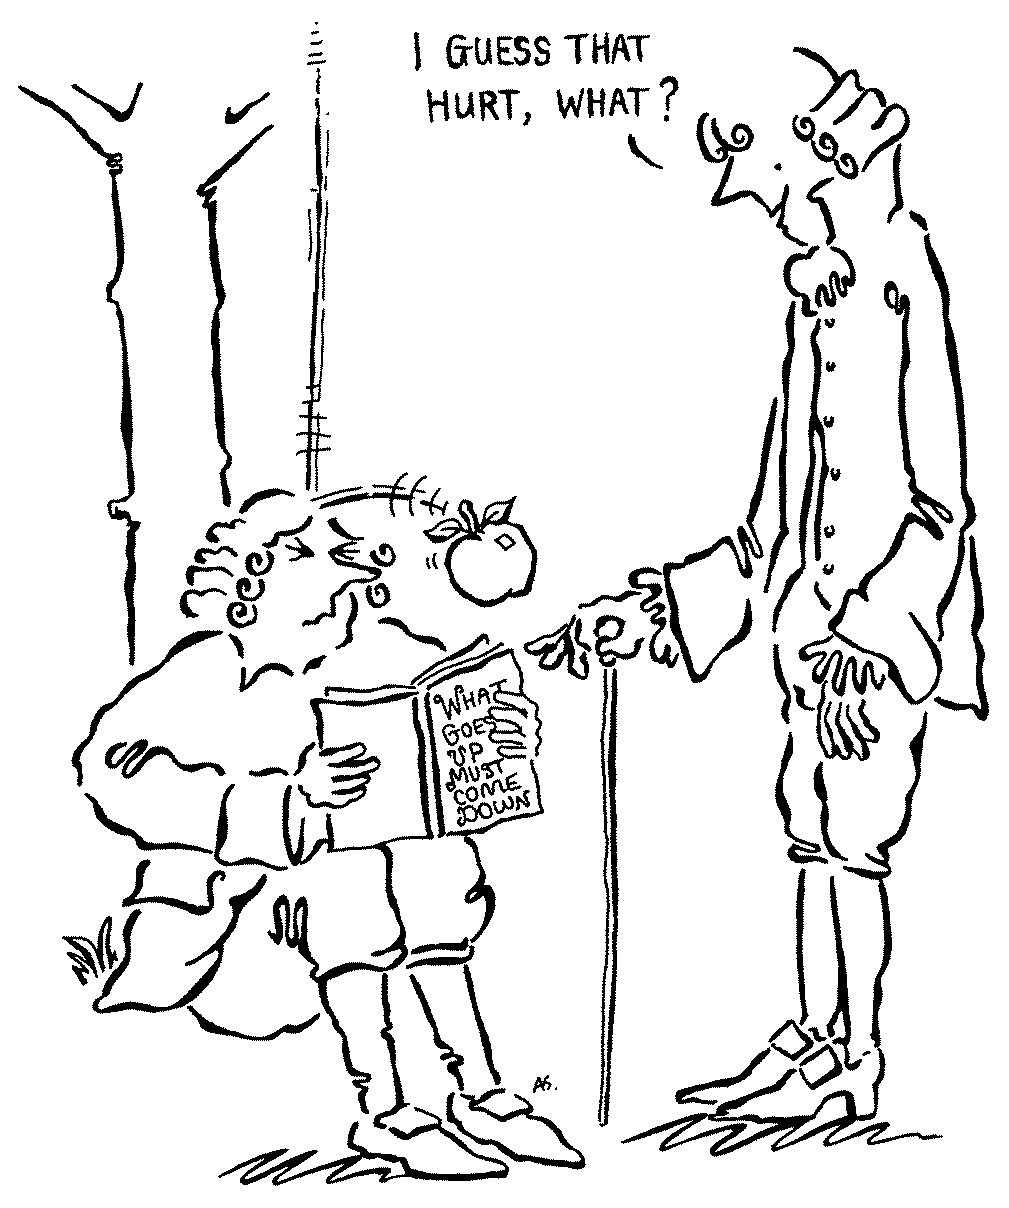
\includegraphics[width=0.60\textwidth]{./Figures/quote.png}

\noindent\enquote{\itshape No great discovery was ever made without a bold guess.}\bigbreak
\end{center}

\begin{flushright}
\textbf{Newton, Sir Isaac} \linebreak
In W.I.B. Beveridge \linebreak
\emph{The Art of Scientific Investigation} \linebreak
Scientist (p. 145)
\end{flushright}

%----------------------------------------------------------------------------------------
%	ABSTRACT PAGE
%----------------------------------------------------------------------------------------

\begin{abstract}
\addchaptertocentry{\abstractname} % Add the abstract to the table of contents

Carbon nano-wires are versatile materials composed of carbon chains with a wide range of applications due to their high conductivity. Regardless of the high interest in the implementation of carbon nano-wires in several applications and devices, no feasible processes have been developed to fabricate carbon nano-wires with spatial control at a reasonable cost. Carbon nano-wires have been fabricated with the use of a photoresist, but little is known about polymers that can produce more conductive carbon nano-wires after pyrolysis. Various polymer solutions have been tested in near field electrospinning (NFES) and photopolymerization separately, however, few have been tested for nano-wire fabrication purposes through pyrolysis. The intention behind the thesis proposal is to implement rheology analyses of different polymer solutions to determine if they can be easily electrospun at low voltages and then fabricate nano-wires with them. This thesis work arises from the need to test a greater variety of polymers with the goal to design a polymer solution to fabricate carbon nano-wires with better conductivity than the current SU-8 polymeric nano-fibers. The research process will include the design of polymer solutions that can be electrospun, photopolymerized, and then pyrolyzed into conducting carbon nanowires. On the other hand, it is intended to engineer a newly designed polymer solution to achieve mass scale manufacturing of conductive carbon nano-wires in an inexpensive, continuous, simple and reproducible manner as central components for nano-sensors. \\

\noindent
\textbf{keywords:} \keywordnames
\end{abstract}

%----------------------------------------------------------------------------------------
%	ACKNOWLEDGEMENTS
%----------------------------------------------------------------------------------------

\begin{acknowledgements}
\addchaptertocentry{\acknowledgementname} % Add the acknowledgements to the table of contents
There are a number of people without whom this thesis might not have been written,
and to whom I am greatly indebted.\\

% To my mother, Helena, who continues to learn, grow and develop and who has been a source of encouragement and inspiration to me throughout my life, a very special thank you for providing a ‘writing space’ and for nurturing me through the months of writing. And also for the myriad of ways in which, throughout my life, you have actively supported me in my determination to find and realise my potential, and to make this contribution to our world.\\

% To my mother-in-law, Maryam, known only briefly but loved and missed, who represented to me ‘living proof’ of Black women’s ability to redefine and recreate our lives despite, and maybe even because of, the tremendously constraining, oppressive and repressive situations in which we often exist.\\

% To my dear husband, Bala who remains willing to engage with the struggle, and ensuing discomfort, of having a partner who refuses to accept the given role of the "Black woman" and is actively engaged in redefining and redesigning that role. A very special thank you for your practical and emotional support as I added the roles of wife and then mother, to the competing demands of business, work, study and personal development.\\

% Thanks to dear Kamal and Azaria, for being so supportive - even when being ‘without Mum’ was hard, and for your help with the bibliography and diagrams. This work is for, and because of you and all the generations to come. It is dedicated to all our journeys in learning to thrive.\\

% It is also dedicated to Josephine - friend, ‘sister’, colleague, ‘co- traveller’ and researcher - who knowingly and unknowingly- led me to an understanding of some of the more subtle challenges to our ability to thrive. If our attempts to claim our right to speak our truth, and to unravel and follow the threads through which our oppression is maintained, and are instrumental in helping one other Black woman from ‘going over the edge’ - in which sight we continuously live our lives - perhaps, it might be seen that your invaluable contribution to the attainment of many of the insights gained was worth it. It is also written in honour of all our my grandmothers, and their mothers, and grandmothers, and to all our and mothers and grandmothers, who though not marked by history struggled so heroically to resist the definitions attributed to them by the dominant system and communicate messages of hope and expectation. I am also very grateful to Maya Angelou, for the inspiration she has been to methrough her writings, poetry readings and as a living representation of a woman thriving. Thanks to Mary Washington, Alice Walker, Jackie Kay, Buchi Emecheta, Toni Cade, Lauretta Ngobo, bell hooks, and other Black women writers of the 1980’s, who in telling stories for and about us validated me and my experiences in ways I cannot begin to explain here.\\

% Loving thanks to my friends and learning partners, Agnes, Susan, Ulana and Namonya, who played such important roles along the journey, as we mutually engaged in making sense of the various challenges we faced and in providing encouragement to each other at those times when it seemed impossible to continue.

I offer my gratitude and appreciation to my supervisors, \supname and \cosupname, for the deft ways in which you lovingly challenged and supported me through out the whole of this work - knowing when to push and when to let up. I offer special thanks to those who supported me in the mechanics of producing this thesis. \supname, for reading and rereading drafts, editing and proofing, typing and helping me get ‘unstuck’ with this thesis on many occasions. And Braulio and Arnoldo for ‘rescuing’ me at those times when I was almost defeated by the laboratory equipment.

\end{acknowledgements}

%----------------------------------------------------------------------------------------
%	LIST OF CONTENTS/FIGURES/TABLES PAGES
%----------------------------------------------------------------------------------------

\tableofcontents % Prints the main table of contents

\listoffigures % Prints the list of figures

\listoftables % Prints the list of tables

%----------------------------------------------------------------------------------------
%	ABBREVIATIONS
%----------------------------------------------------------------------------------------

\begin{abbreviations}{ll} % Include a list of abbreviations (a table of two columns)

\textbf{CEM} & \textbf{C}ampus \textbf{E}stado de \textbf{M}éxico\\

\textbf{CNWs} & \textbf{C}arbon \textbf{N}ano-\textbf{w}ire\textbf{s}\\

\textbf{DC} & \textbf{D}irect \textbf{C}urrent\\

\textbf{EMS} & \textbf{E}lectro\textbf{m}echanical \textbf{S}pinning\\

\textbf{FFES} & \textbf{F}ar \textbf{F}ield de \textbf{E}lectro\textbf{s}pinning\\

\textbf{ITESM} & \textbf{I}nstituto \textbf{T}ecnonólogico y de \textbf{E}studios \textbf{S}uperiores de \textbf{M}onterrey\\

\textbf{MA} & \textbf{Ma}ssachusetts\\

\textbf{MEMS} & \textbf{M}icro\textbf{e}lectro\textbf{m}echanical \textbf{S}ystems\\

\textbf{MNT} & \textbf{M}aestría en \textbf{N}ano\textbf{t}ecnología \emph{(Master of Science in Nanotechnology)}\\

\textbf{MTY} & \textbf{M}on\textbf{t}erre\textbf{y} \emph{or} Campus \textbf{M}on\textbf{t}erre\textbf{y}\\

\textbf{NFES} & \textbf{N}ear \textbf{F}ield de \textbf{E}lectro\textbf{s}pinning\\

\textbf{USA} & \textbf{U}nited \textbf{S}tates of \textbf{A}merica\\

\textbf{UV} & \textbf{U}ltra\textbf{v}iolet\\

\end{abbreviations}

%----------------------------------------------------------------------------------------
%	SYMBOLS
%----------------------------------------------------------------------------------------

\begin{symbols}{lll} % Include a list of Symbols (a three column table)

%$a$ & distance & \si{\meter} \\
%$P$ & power & \si{\watt} (\si{\joule\per\second}) \\
Symbol & Name & Unit \\

\addlinespace % Gap to separate the Roman symbols from the Greek

$\omega$ & angular frequency & \si{\radian} \\

\end{symbols}

%----------------------------------------------------------------------------------------
%	PHYSICAL CONSTANTS/OTHER DEFINITIONS
%----------------------------------------------------------------------------------------

%\begin{constants}{lr@{${}={}$}l} % The list of physical constants is a three column table

% The \SI{}{} command is provided by the siunitx package, see its documentation for instructions on how to use it

%Speed of Light & $c_{0}$ & \SI{2.99792458e8}{\meter\per\second} (exact)\\
%Constant Name & $Symbol$ & $Constant Value$ with units\\

%\end{constants}

%----------------------------------------------------------------------------------------
%	THESIS CONTENT - CHAPTERS
%----------------------------------------------------------------------------------------

\mainmatter % Begin numeric (1,2,3...) page numbering

\pagestyle{thesis} % Return the page headers back to the "thesis" style

% Include the chapters of the thesis as separate files from the Chapters folder
% Uncomment the lines as you write the chapters

\setlength{\parskip}{1.5em} % Paragraph spacing
%\RaggedRight
{\fontsize{12}{15} \selectfont

% Chapter Template

\chapter{Introduction} % Main chapter title

\label{Chapter:1}

Carbon nano-materials are subjected to great interest for research purposes due to their various potential applications in diverse areas that take advantage of the nano-scale properties. Carbon nano-materials are suitable for catalysis, adsorption, carbon capture, energy and hydrogen storage, drug delivery, bio-sensing, and cancer detection. Some matchless properties that allow carbon nano-materials to be utilized within multiple functionalities include high porosity, distinguished structures, uniform morphologies, high stability, high magnetic properties, and high conductivity. \cite{Siddiqui2019, McCreery2008, Geim2011, Zhu2010, Katsnelson2008, Li2008, Geim2007, Geim2009}

This document bestows a thesis project to perform research to engineer a polymer solution to achieve mass scale manufacturing of high conductive carbon nano-wires with a reduced diameter in an inexpensive, continuous, simple and reproducible manner. The research intends to involve several manufacturing processes such as near field electrospinning, photo-polymerization, pyrolization, and carbonization, as they have shown to be promising methods for the fabrication of carbon nano-materials. \cite{Cardenas2017} See Figure \ref{fig:fabricationFlowChart}. A number of processes have been developed for specific purposes of polymeric nano-fibres, some include surface deposition, composites, and chemical adjustments. Polymeric nano-fibers must be also pyrolyzed to generate carbon nano-wires with conductive capabilities \cite{Madou2011} for electrochemical sensing and energy storage purposes.

\begin{figure}[th]
\centering
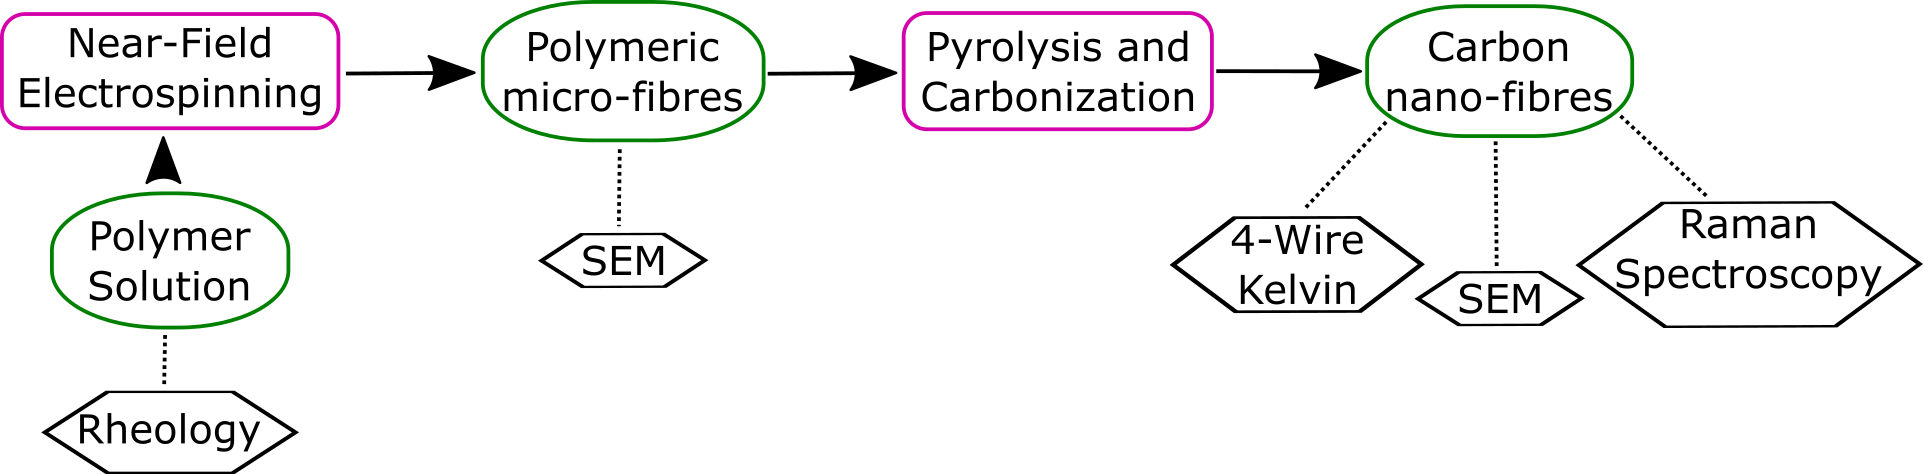
\includegraphics[width=1.0\textwidth]{./Figures/FabricationProcess2.png}
\decoRule
\caption[Fabrication Process]{Fabrication process and characterization techniques of conductive carbon nano-wires to achieve through the dissertation.}
\label{fig:fabricationFlowChart}
\end{figure}

Nanotechnology has led to the study of different polymer patterning techniques to integrate carbon nano-wires structures. One technique is known as far-field electrospinning (FFES), a process in which electrified jets of polymer solution are dispensed to synthesize nano-fibres which are then pyrolyzed at high temperatures. One sub-technique derived from electrospinning is near-field electromechanical spinning or NFEMS. Unlike FFES, NFEMS has proved to deliver high control in patterning polymeric nano-fibres. \cite{Cardenas2017}

The proposal is to continue the previous work done in regards to the synthesis of carbon nano-wires. Previous work includes the fabrication of suspended carbon nano-wires by two methods: electro-mechanical spinning and multiple-photon polymerization with a photoresist. \cite{Cardenas2017, Flores2017} This work is intended to focus on electro-mechanical spinning processes only, to bring off polymer solutions that can be electrospun by NFEMS, photo-polymerized and pyrolyzed into conducting carbon nano-wires. The polymer solutions described by Cárdenas and Flores \cite{Flores2017, Cardenas2017} are to be amended to achieve the goal mentioned in the previous statement.

Traditional near-field electrospinning or NFES allows large scale manufacturability combined with spatial control of material deposition. \cite{Madou2011} However, the reported efforts required the use of electric fields in excess of 200 kV/m for continuous operation, resulting in limited control for nano-fiber patterning in traditional NFES processes. Madou et al. \cite{Madou2011} conclude that the current state-of-the-art synthesis processes for polymer nano-fibers lack to yield precise, inexpensive, fast, and continuous manufacturing properties.

%----------------------------------------------------------------------------------------
%	SECTION 1
%----------------------------------------------------------------------------------------
\section{Carbon Nanowires Research Developments in Terms of Published Papers, Synthesis and Fabrication}

% \cite{Rauti2019}

Nanotechnology ability to control and piece together materials at the nano-scale has enabled the development of various carbon nano-materials and carbon nano-structures, such as nano-dots, nano-fibres, nano-tubes and nano-wires. \cite{Posthuma-Trumpie2012, Zhang2009, DeVolder2011, Cao2011} This chapter bestows on the applications at the micro-scale and nano-scale levels, as well as the current research of carbon-based nano-materials (CBNs).

\subsection{Carbon and carbon-based nanomaterials}

Carbon is a versatile element capable to form a number of bonds with other elements or with itself. Furthermore, carbon orbitals have the ability to hybridize in sp1, sp2 and sp3 configurations, hence the existence of different types of allotropes, see Figure \ref{fig:carbonAllotropes}. To date, the three naturally occurring allotropes of carbon (diamond, amorphous carbon and graphite), have been joined by additional ones deriving from synthetic processes (such as graphene, carbon nano-tubes, fullerenes, carbon nanohorns, nanodiamonds) [ [12]; Fig. 1].

The interest in CBNs has increased exponentially in the last
decades, first with the discovery offullerenes (1985), then with that of carbon nanotubes (CNTs; 1991) and finally with the synthesis of graphene (GR) (2004).

The properties of these CBNs make them widely used in many
fields ranging from material science [13], energy production and storage [14], environmental sciences [15,16], biology [17-19] and medicine [20,21]. Table 1 summarizes the main properties of the most common CBNs [22-25]:

Among the many carbon nanomaterials, CNTs and GR are currently the most popular representatives and have been extensively studied for their excellent mechanical strength, electrical and thermal conductivity and optical properties. The Young's modulus and tensile strength of CNTs and GR can reach 1 TPa and 130 GPa respectively [20,21]. Carrier mobility of graphene is around 860 $cm^{2} V^{-1} s^{-1}$ (hole mobility of 844 $cm^{2} V^{-1} s^{-1}$ and carrier mobility of 866 $cm^{2} V^{-1} s^{-1}$), and the current density of metallic CNTs is orders of magnitude higher than those of metals such as copper [26,27]. Thermal conductivities of CNTs and GR are about 3000e3500W/mK and 5000 W/mK respectively [28]. The light absorption ratio of single-layer graphene is limited to 2.5\% [29]. A large amount of the research efforts were focused on exploiting these properties for various applications including electronics, biological engineering, filtration, lightweight/strong composite materials, photovoltaic and energy storage [30-32]. CNTs and GR are naturally good electrical conductors and their biocompatibility can be modulated [33], making them good candidates for improving electrodes for neural interfaces. Electrical recording or stimulation of nerve cells is widely employed in neural prostheses (for hearing, vision, and limb-movement recovery), in clinical therapies (treating Parkinson's disease, dystonia, and chronic pain), as well as in basic neuroscience studies. In all these applications, electrodes of various shapes and dimensions stimulate and/or record neuronal activity to directly modulate behavior or to interface machine. The performance of the electrodes can be significantly improved by implementing the device with nanomaterial-based coatings (such as CBNs), since their high surface area can drastically increase charge injection capacity and decrease the interfacial impedance with neurons [34].

%%%
It is well known that the morphology of the electroactive material play an important role in electrochemical systems, once the intimate contact at the electrode/electrolyte interface is crucial to guarantee the charge transfer process [11,12]. In this sense, nanostructured electroactive materials such as nanorods [13], nanofiber [14], nanoflowers [15,16], nanowires [17,18], among others [19,20], are being widely used to obtain improved electrochemical properties such as higher charge/discharge rate and improved task to accommodate stress due to volume changes occasioned by intercalation process.

\subsection{Carbon nanowires}

Carbon nanofibers (CNFs) have been classified as linear, sp2-based discontinuous filaments, where the aspect ratio is greater than 100 [207]. Depending on the angle of the graphene layers that compose the filament, CNFs have even been classified as stacked (graphene layers stacked perpendicularly to the fiber axis) or herringbone/cupstacked (graphene layers stacked at an angle between parallel and perpendicular to the fiber axis) [208].

%%%
Nanowires are one-dimensional, anisotropic structures, small in diameter, and large in surface-to-volume ratio. These characteristics confer to the nanowires special physical properties than those of traditional scale and dimensionality materials, such as electrical, optical thermal and mechanical properties. However, this make this kind of materials to have properties deeply dependent on their surface condition and geometrical configuration [21]. The transport properties in the 1D nanostructures like the nanowires are affected by wire diameter, surface conditions, crystal quality, crystallographic orientation and material composition, thus the synthesis conditions are a crucial factor to obtain reproducible and high-quality nanowires for different application [21].

The typical lengths and diameters of carbon nanofibers are in the ranges of 5e100mm and 5e500 nm, respectively [209]. CNTs and GR are the most studied carbon nanomaterials for neural interfaces, however CNFs are also attractive in bio-interfacing developments due to their chemical and physical properties [1]: CNFs are chemically stable and inert in physiological environment [2], they are biocompatible for long-term implantation due to CNFs solid carbon skeleton [3], they are electrically robust and conductive for signal detection [4], they can be manufactured into 3D structures allowing intra-tissue and intracellular penetration [210], CNFs possess high surface-to-volume ratio, which greatly reduces electrical impedance, and [5] ultra-micro scale sizes that provide high spatial resolution. CNFs have been applied as promising materials in many fields, such as energy conversion and storage, reinforcement of composites and self-sensing devices.

In addition, CNF based materials have been developed as electroconductive scaffolds for neural tissues to facilitate communication through neural interfaces. Electrical fields are able to enhance and direct nerve growth [211], therefore electroconductive scaffolds have been applied to enhance the nerve regeneration process, not only providing physical support for cell growth but also delivering the functional stimulus. CNFs may represent novel, versatile neural interfaces, being capable of dual-mode operation by detecting electrophysiological and neurochemical signals, not only at the extracellular level with high spatial resolution, but also at the intracellular level by penetrating into single neurons [9].

Despite the longstanding experience on these nanomaterials and the deep knowledge of the CNFs-neuron interface in vitro, in vivo experiments on their possible application for the treatment of brain and spinal cord injuries or diseases are still limited to few examples [53,212,213]. In the first report CNFs impregnated with subventricular stem cells were employed to promote neuroregeneration after experimental stroke [53]. The animals receiving the CNF-based treatment show reduction of the infarcted volume as well as recovery ofmotor and somatosensory activity. These data indicate that CNFs are optimal support material for neuronal tissue regeneration [53].

Recently, Guo and collaborators [104] developed a polymer-based neural probe with CNFs composites as recording electrodes via the thermal drawing process [213]. They demonstrated that in situ CNFs alignment was achieved during the thermal drawing, which contributes to a drastic improvement of electrical conductivity by 2 orders of magnitude compared to a conventional polymer electrode. The resulting neural probe has a miniature footprint, with a recording site reduced in size to match single neuron, yet maintaining impedance value able to capture neural signals. In chronic settings, long-term reliable electrophysiological recordings with single-spike resolution and minimal tissue response over extended period of implantation in wild-type mice were shown [213].

%%%
Nanostructured materials are particularly good for supercapacitor applications, providing high surface area, which leads to a high specific capacitance [22]. Compared to 3D and 2D materials, 1D nanostructures have smaller dimension and higher aspect ratio, improving the transport of electrical carriers in one controllable direction and also can be exploited as elements in different kinds of nanodevices [23]. In this way, nanowires have been satisfactorily used in supercapacitor electrodes due to their reduced ion diffusion path in comparison with 2D and 3D nanostructures, leading in higher charge/discharge rates [22,24].

%%%
Amongst the innumerous materials used to obtain 1D nanostructures, such as, carbon, silicon, transition metal oxides, the 1D nanostructured conductive polymers are a important group to fabricate energy storage devices, due their attractive characteristic, such as, mechanical properties, electrical conductivity, low cost, easy processing, high surface area and unique electroactive behavior, including high voltage window and high-doping rate during charge-discharge process [25]. During the charge/discharge process in the conducting polymer occur the insertion/desertion ions from the electrolyte in the polymer backbone that could result in swelling and shrinkage of the polymer chain, leading to mechanical degradation of the electrodes and fading the electrochemical performance [26]. An alternative to diminishment this drawback of the conductive polymers is fabricate composites that could improve the stability and conductivity of the electrodes [27].

%%%
In this way, composites based on conducting polymers and carbon or metal oxides materials in a nanowire architecture are a good strategy to develop high-performance devices due to the combination of the electrochemical properties of the polymer and/or composites with the morphological advantages of the nanowires. These combination results in large interface between electrode/electrolyte, effective electronic transport pathway, short ion diffusion distance and easy relaxation strain, which could improve both capacity/capacitance and rate performance of battery and supercapacitors devices, respectively [28]. Furthermore, the mechanical properties of nanowires allow the development of flexible devices, that require materials with versatile functionalities including high flexibility and foldability without losing its high power and energy density and long lifetime [29].

\subsection{Nanowires synthesis}

%%%
Numerous methods to prepare nanowires, which include template-assisted synthesis [30], vapor–liquid-solid (VLS) [31], electrodeposition [32], electrospinning [33], hydrothermal [34], also hierarchical arrangement techniques [35–37] to organize the nanowires have been studies in the last ten years. Nanowires based on organic, inorganic or hybrid materials have been applied in order to get single or composites nanomaterials for innumerous purposes, such as chemical and biochemical sensing devices, thermoelectric, optical, magnetic and electrical application. In this section, we are focusing on the synthesis of conducting polymer and composites to develop materials in nanowires architectures.

\subsubsection{Synthesis of conducting polymer nanowires}



\subsection{\emph{conclude that NFES is the way to go}}




%----------------------------------------------------------------------------------------
%	SECTION 2
%----------------------------------------------------------------------------------------
\section{Problem definition and motivation}

%Qué metodos se han utilizado? (SU-8)
%Porqué se quiere fabricar las fibras de carbono
%Para qué aplicaciones se han usado
%Porqué es importante la conductividad
%Porqué es importante que sea puro carbono

Carbon nanowires have been fabricated with a photoresist by multiple-photon polymerization techniques. However little is known about polymers that can produce conductive carbon nano-wires after pyrolysis, as it is generally believed that most polymers do not form significant amounts of graphitic carbon when carbonized.
%The lack of research relays on the fact that in the past years, it was assumed that most polymers are non-graphitic through pyrolysis \cite{Franklin1951}.
In the past years, photopolymerization processes have been applied to the fabrication of nano-structures with the use of an epoxy based photoresist. \cite{Boer2014} Photopolymerization techniques deliver patterning resolutions with nano-scale tolerances through two-photon lithography for the production of highly detailed structures \cite{Hribar2014}.

On the other hand, electrospinning has been acknowledged as a process with promising results at nano-structure fabrication \cite{Boer2014}, yet there is little research regarding the implementation of electrospinning for the fabrication of carbon nano-wires. Electrospinning has the potential to be a more straightforward process for the design and fabrication of nano-structures, as it can achieve mass scale manufacturing in a continuous, simple and reproducible manner. Cardenas \cite{Cardenas2017} showed that electrospinning can be implemented with ease for carbon nano-wire synthesis. Mechano-electrospinning, a new variant of electrospinning shows promising results in the production of ordered carbon nano-wires. As stated in \cite{Cardenas2017}, mechano-electrospinning is an early technology invention and brings new challenges, such as the reproducibility of carbon nano-wire production. Furthermore, the study of a new fabrication process to produce carbon nanowires that involves mechano-electrospinning will enable spatial control of the structures' patterning.

Since electrospinning seems to be a better alternative for carbon nano-wire fabrication processes; and for that purpose of its implementation, it is required to develop polymer solutions that can be mechano-electrospun, photopolymerized and pyrolyzed into conducting carbon nano-wires. Carbon nano-materials have been subjected to research due to their various potential applications in diverse areas that take advantage of the nano-scale properties. \cite{Siddiqui2019} Carbon nano-materials are suitable for the catalysis, adsorption, carbon capture, energy and hydrogen storage, drug delivery, bio-sensing and cancer detection. \cite{Siddiqui2019} However most applications are not currently feasible due to the lack of a continuous, simple and reproducible fabrication method with inexpensive processes. With the newly designed polymer solution, it would be possible to produce carbon nano-wires in large quantities, and therefore more applications will become feasible. On the other hand, the new technique will overcome some limitations of other methods such as lithography currently has. For instance, patterns created by lithography processes cannot be originated, only replicated, all constituent points of the pattern can only be addressed at the same time, and the process requires the pattern to be encoded into a mask. \cite{Landis2011}

%----------------------------------------------------------------------------------------
%	SECTION 3
%----------------------------------------------------------------------------------------
\section{Hypothesis}

The rheological properties of polymer solutions along with synthesis parameters (stage velocity, voltage, dispense rate) can be amended through rheological analyses to obtain a low voltage electrospun-able, photopolymerizable and graphitizable fibers for the fabrication conductive of carbon nano-wires with specified dimensions (diameter and length). The rheological properties of polymer solutions along with synthesis parameters are to be amended by replacing the PEO (Poly(ethylene) oxide) component within the existing polymer solutions described in Flores \cite{Flores2017} and Cardenas \cite{Cardenas2017} work. PEO is to be replaced as its only purpose is to allow the electrospinning process to take place, but no benefit is obtained from it after pyrolysis.

%----------------------------------------------------------------------------------------
%	SECTION 4
%----------------------------------------------------------------------------------------
\section{Research Questions}

\begin{itemize}
	\item{
	Is there any evidence of conductive carbon nano-wire fabrication though electrospun-able and pyrozable polymer solutions?
	}
	\item{
	What are the process parameters to consider/control for the fabrication processes of carbon nano-wires? 
	}
	\item{
	What rheological properties are to be controlled/tested to deliver an electrospun-able and pyrozable polymer solution?	
	}
	\item{
	Are there any efforts employed to the design of polymer solutions that can be electrospun, photopolymerized, and pyrolyzed into conducting carbon nanowires?
	}
	\item{
	What are the optimal fabrication parameters for the synthesis of carbon nano-wires through near-field electromechanical spinning?	
	}
	\item{
	What materials can be used to ease the electrospinning process and favor the carbon nano-wire properties after pyrolysis? 
	}
\end{itemize}

%----------------------------------------------------------------------------------------
%	SECTION 5
%----------------------------------------------------------------------------------------
\section{Objectives}

\subsection{General objective}
Study the practice and feasibility of a new fabrication process to achieve mass scale manufacturing of carbon nano-wires in an inexpensive, continuous, simple and reproducible manner; by the integration of mechano-electrospinning technique.

\subsection{Specific objectives}

\begin{itemize}
	\item{
	Design polymer solutions that can be electrospun by NFES, photopolymerized, and then pyrolyzed.
    }
    \item{
    Through rheological analyses, determine if polymer solutions can be easily employed for conducting carbon nano-wire synthesis.
    }
    \item{
    Determine and control the polymer solution rheological properties along with the process parameters of carbon nano-wire synthesis.
    }
    \item{
    Discover a PEO-similar material to allow the electrospinning process as well as input favourable properties to the carbon nano-wire yield.
    }
\end{itemize}

%----------------------------------------------------------------------------------------
%	SECTION 6
%----------------------------------------------------------------------------------------
\section{Dissertation Outline}



\chapter{Near-Field Electrospinning as an Affordable Way to Gain Spatial Control} % Main chapter title

\label{Chapter:2}

%----------------------------------------------------------------------------------------
%	SECTION 1
%----------------------------------------------------------------------------------------
\section{Review of Polymer Solutions for NFES with Spatial Control}

Near-field electrospinning (NFES) is identified to be a technique able to fabricate polymer nano and micro fibers with accurate placement. In the past years (2006-2020), several polymer solutions have been successfully electrospun into fibers through several variants of the conventional NFES process. Each NFES variant intents to tailor the process parameters in order to improve the fibers' properties. 

Even though electrospinning is an old invention \unskip~\cite{527120:12073288}, it is currently a trending topic among researchers \unskip~\cite{527120:12073453,527120:12073495,527120:12073496}. One of the reasons electrospinning is to be studied is its potential to fabricate polymer nano fibers from a variety of polymers. The technique allows the production of thin continuous fibers with ease, with micro and sub-micrometer diameters, which is something difficult to achieve by other techniques. Furthermore, the basic setup can be modified with ease to fabricate different fibers with diversified functionalities with different materials. The produced fibers can be aligned or unaligned. Besides, the electrospinning equipment is inexpensive and of small size, compared to the equipment of standard spinning techniques\unskip~\cite{527120:12073538}. On the other hand, the understanding of the electrospinning process has improved in the last years.

Current literature dictates the typical spinning setup is comprised by three main components: a polymer reservoir, a fiber collector, and some way to dispense the fibers onto the collector. The spinning process is an electro-hydrodynamic (EHD) technique that yields continuous polymer fibers. Other EHD techniques are spraying and atomization which produce polymer droplets and polymer particles respectively, seeFigure~\ref{f-02e0e3cf88d6}.

\bgroup
%\fixFloatSize{images/514dfac6-849d-4905-8e40-7adfafc93b5f-uimg_ehd_techniques.png}
\begin{figure}[!htbp]
\centering \makeatletter\IfFileExists{./images/514dfac6-849d-4905-8e40-7adfafc93b5f-uimg_ehd_techniques.png}{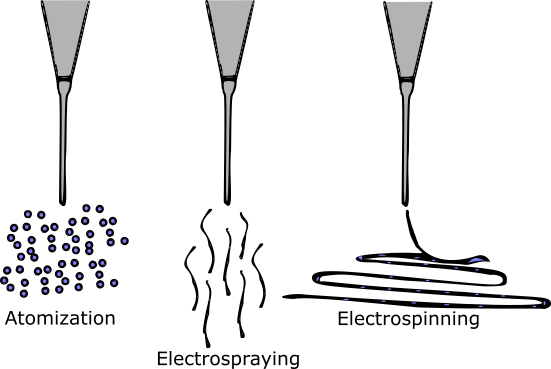
\includegraphics[scale=0.65]{./images/514dfac6-849d-4905-8e40-7adfafc93b5f-uimg_ehd_techniques.png}}{}
\makeatother 
\caption{{Electrohydro-dynamic techniques}}
\label{f-02e0e3cf88d6}
\end{figure}
\egroup

\subsection{Stretching forces}



\subsubsection{Electric Field}Electrospinning (electrostatic fiber spinning) is a fiber fabrication approach that implements an electric field produce fibers by an electrical potential difference between the syringe needle and the collector. With the influence of high electric fields, the fibers are prone to brake into separate layers due to the whipping instabilities as the jet travels to the substrate. The instability can be mitigated by adding additional ring electrodes between the spinneret and the grounded collector. \unskip~\cite{527120:13915304}

The typical electrospinning setup applies an electrostatic charge to the polymer fluid at the tip of the needle nozzle, which results in the formation of the Taylor cone \unskip~\cite{527120:13659828}, from which a single polymer jet is ejected to the grounded collector. From the Taylor cone, the supplied polymer jet (typically a polymer solution) accelerates and reduces in diameter. The fiber finally develops with the complete solvent evaporation. Electrospun fibers are prone to splitting with the increase in acceleration due to high applied voltages, where multiple fibers are yield in a process known as electrospraying \unskip~\cite{527120:13659925}.

The electrospinning process starts with charging a polymer solution droplet. When a polymer solution is administrated with a syringe pump, solution droplets will fall under the influence of gravity. The solution dripping stops when the electric field is strong enough to break the solution's surface tension, causing the droplet to change shape forming a polymer solution jet\unskip~\cite{527120:12033655}.

Shin et al. \unskip~\cite{527120:13659926} reported that the growth of the whipping instability is one important element within the electrospinning technique. As detailed in Shin's work, weak electric fields produce a single uniformly thinning jet, and strong electric fields the jet becomes unstable after traveling a short distance.



\paragraph{High voltage power supply: DC \& AC - }Direct current (DC) is typically used in electrospinning with the electrons flowing in one direction. Alternate current (AC) implementations are also studied as the AC creates a change in the direction of the current flow. Kessick et al.\unskip~\cite{527120:13444381} demonstrated the implementation of AC power supplies in the production of polymer fibers.

The AC electrospinning setup is similar to that for the DC variant. AC electrospinning apparatus do not require a grounded collector as the current alternates. In AC, the produced fibers are prone to carry an electric charge, while those generated shortly after have an opposite charge. The difference in charges lead the fibers to discharge on each other, creating an aerogel plume of fibers\unskip~\cite{527120:16885570}. The optimal AC frequency depends on the materials used and is typically within  $50Hz $ and  $1kHz $\unskip~\cite{527120:13443405}.

The AC technique has been studied for drug loaded related applications. Balogh et al. \unskip~\cite{527120:13445177} compared fibers fabricated by DC and AC spinning techniques. Their work reports that AC and DC electrospinning can produce fibers with all three polymers, where the AC process allowed the implementation of faster flow rates than in the DC setup. The DC electrospinning technique generated fibers with a maximum flow rate of 5 $ml/h $; on the other hand, the AC setup allowed an increase in flow rate up to 40 $ml/h $.



\subsubsection{Centrifugal force}The spinning processes require the implementation of a force to break the polymer source into a polymer jet. Centrifugal spinning intends to produce fibers by the use of a rotating polymer source. The centrifugal force generated from typical rotatory speeds above $2000 rpm $, results in fiber formation. \unskip~\cite{527120:13535559,527120:13535561}.


\bgroup
%\fixFloatSize{./images/19c94c11-1ae0-47bd-95ef-4dc5ceedc20d-uimg_gyro_es.png}
\begin{figure}[!htbp]
\centering \makeatletter\IfFileExists{./images/19c94c11-1ae0-47bd-95ef-4dc5ceedc20d-uimg_gyro_es.png}{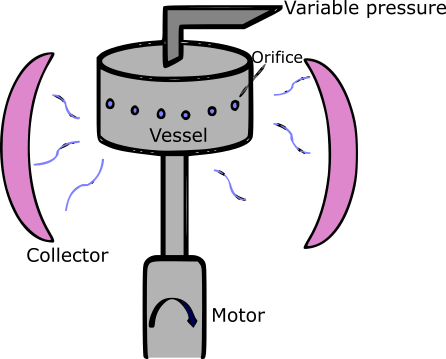
\includegraphics[scale=0.65]{./images/19c94c11-1ae0-47bd-95ef-4dc5ceedc20d-uimg_gyro_es.png}}{}
\makeatother 
\caption{{Typical setup used in pressurized gyration processes}}
\label{f-7cf6ac702e28}
\end{figure}
\egroup
The centrifugal force technique has been applied to polymer solutions and melts. This approach is used in applications were the precise deposition of the fibers is not relevant and production rate is to be maximized \unskip~\cite{527120:13535894}.  Efforts in centrifugal spinning are focused on drug delivery applications. Zander \unskip~\cite{527120:13535977} fabricated polycaprolactone (PCL) fibers using the solution and melt variants of the centrifugal approach. Zander's fibers were produced with rotatory speed between three and 18 thousand revolutions per minute with $10 \mu m $ in diameter. 

On the other hand, PCL and PVP fibers were generated by Amalorpava et al. \unskip~\cite{527120:13536089}.  Amalorpava achieved sub micron/size fiber diameters for drug release purposes and bacteria growth inhibition properties. Literature\unskip~\cite{527120:13536446} has shown that centrifugal approach has a simple setup that promises a large scale fabrication of fibers.

In some cases the centrifugal force implementations and pressurized gyration can be combined with an electric field. The implementation of two stretching forces (centrifugal and electrical forces), can help solvent evaporation\unskip~\cite{527120:13536560}. Centrifugal electrospinning implements the same setup as the standard centrifugal spinning with the addition of a high voltage power supply between the rotating dispensing nozzle and the collector. The combined method has evidence to yield parallel fibers\unskip~\cite{527120:13536841,527120:13536900,527120:13537392,527120:13537393} at a higher rate \unskip~\cite{527120:13536841,527120:13536900} than the standard electrospinning approach.



\subsubsection{Blowing forces}Nano fibers can be produced with the implementation of pressurized gas with a polymer solution. The setup used for blow spinning is similar to the one used in coaxial electrospinning, where the polymer precursor is dispensed at a controlled rate. Unlike traditional electrospinning, in the solution blow spinning setup the needle nozzle applies pressurized gas to the polymer solution through an outer spinneret\unskip~\cite{527120:13538056}, see Figure~\ref{f-92361290d8c3}. 


\bgroup
%\fixFloatSize{./images/87246522-4cf1-491f-a45f-cda541854d72-uimg_blow_es.png}
\begin{figure}[!htbp]
\centering \makeatletter\IfFileExists{./images/87246522-4cf1-491f-a45f-cda541854d72-uimg_blow_es.png}{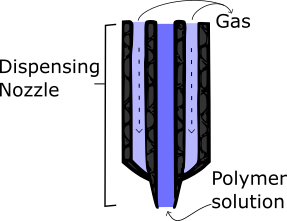
\includegraphics[scale=0.65]{./images/87246522-4cf1-491f-a45f-cda541854d72-uimg_blow_es.png}}{}
\makeatother 
\caption{{Dispensing nozzle used for solution blow spinning or melt blowing. \unskip~\protect\cite{527120:13538056}}}
\label{f-92361290d8c3}
\end{figure}
\egroup
Poly(lactic acid) (PLA) fibers have been produced by solution blow spinning. Oliveira et al. \unskip~\cite{527120:13539278} fabricated the fibers from $6 wt\% $ PLA solutions with progesterone for live stock reproductive cycle regulation applications. On the other hand, Souza et al.\unskip~\cite{527120:13538056} conducted a study to compare the standard electrospinning and the solution blow spinning techniques. Poly(3-hydroxybutyrate-co-3-hydroxyvalerate) were fabricated by both methods. The fibers produced by traditional electrospinning had thicker diameters and the size uniformity was higher in the fibers produced by solution blow spinning. The experimental setup requires a coaxial needle nozzle with a pressurized gas flow along with a potential difference between the dispensing needle and the grounded collector.



\subsubsection{Mechanical force}
\bgroup
%\fixFloatSize{./images/23a9bc42-4d02-4a78-a907-23aeeb2de68a-uimg_meches_process.png}
\begin{figure*}[!htbp]
\centering \makeatletter\IfFileExists{./images/23a9bc42-4d02-4a78-a907-23aeeb2de68a-uimg_meches_process.png}{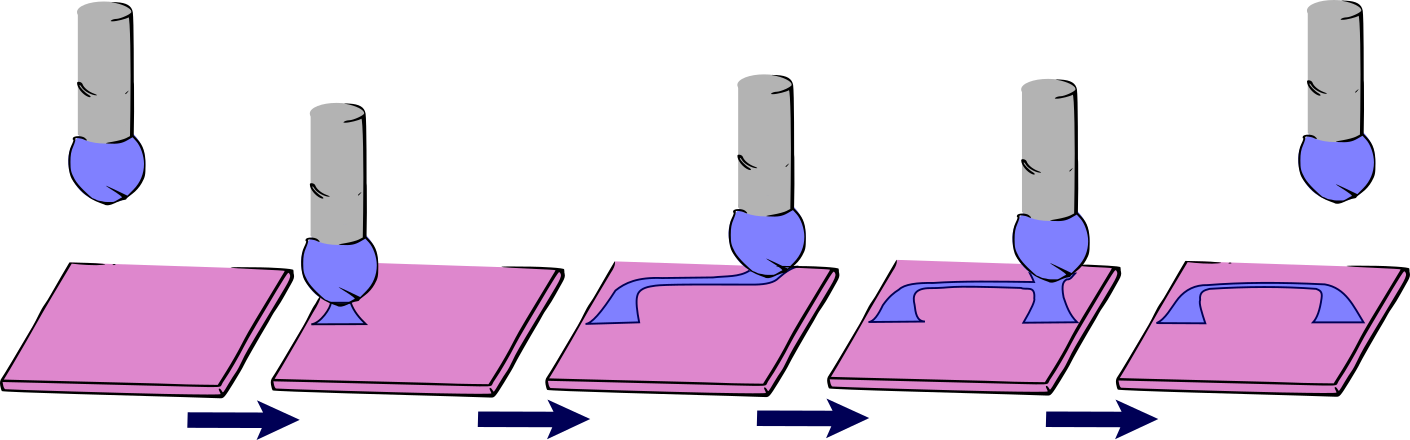
\includegraphics[scale=0.35]{./images/23a9bc42-4d02-4a78-a907-23aeeb2de68a-uimg_meches_process.png}}{}
\makeatother 
\caption{{Typical mechanical fiber drawing process. First the needle makes contact with the substrate to break the polymer drop. Then the needle leaves the substrate and the collector moves to create and deposit the fiber. Once the fiber is written the needle makes contact witht the collector to fix the fiber deposition.}}
\label{f-432d16f420fb}
\end{figure*}
\egroup
Mechanical drawing comprises the simple technique to produce fibers by stretching the polymer solution with a glass pipette. \unskip~\cite{527120:14024998} Nevertheless, the drawing technique is not scalable or with practical applications. \unskip~\cite{527120:14025041} Touch-spinning methods have been developed to introduce a scalable technique for the production of nano fibers where the fiber is created by stretching the polymer precursor with a moving collector, as depicted in Figure~\ref{f-432d16f420fb}. Touch-spinning is another mechanical technique that comprises a moving stage with an embedded glass rod (Figure~\ref{f-f17259e76303}). Where a polymer solution is supplied from a syringe needle such that the tip of the glass rod makes contact with the polymer solution as it rotates, creating fibers. The rotation stretches the fiber, causing the fiber to increase in length and decrease in diameter. The increase in length causes the fiber surface are to increase and therefore making the polymer solution solvent to volatilize, ending with a dry fiber within the collector.


\bgroup
%\fixFloatSize{./images/c33e7bfe-18c6-4765-834e-a85f12cd2621-uimg_touch_process.png}
\begin{figure*}[!htbp]
\centering \makeatletter\IfFileExists{./images/c33e7bfe-18c6-4765-834e-a85f12cd2621-uimg_touch_process.png}{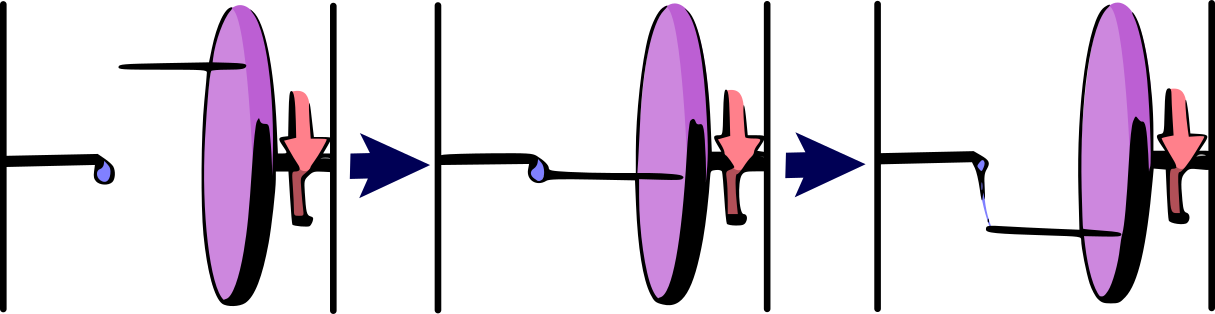
\includegraphics[scale=0.45]{./images/c33e7bfe-18c6-4765-834e-a85f12cd2621-uimg_touch_process.png}}{}
\makeatother 
\caption{{Touch-spinning technique. First rod is attached to a rotating stage and a polymer solution droplet is administrated through a needle. Then the rotating rod 'touches' the polymer precursor. Finally, as the rod rotates, the polymer solution is stretched and creates a fiber between the rod and the needle.}}
\label{f-f17259e76303}
\end{figure*}
\egroup
The touch spinning technique implies that the fiber diameter can be controlled by the moving collector's speed and the polymer solution concentration. The main difference relays on the fact that the touch spinning method implements mechanical control to manipulate and stretch the fibers during the fabrication process, guiding the fiber in the collector enabling better control over fiber alignment.\unskip~\cite{527120:14091959}



\subsubsection{Microfluidic forces}The microfluidic spinning technique manipulates and controls the polymer solution in networks of micrometer channels. The channel network are typically embedded in a microfluidic chip, where the solution deposition rate is controlled by active components (pumps and valves) with a computer. Cheng et al. \unskip~\cite{527120:13656236} compared and combined the microfluidic spinning and electrospinning techniques. Heterogeneous materials and cell patterning within a single microfiber can be designed by the integration microfluidic channels. Therefore, microfluidic spinning is more suitable for cell encapsulation and tissues generation\unskip~\cite{527120:13656236}.

On the other hand, Kang et al. \unskip~\cite{527120:13656548} managed to fabricate micro fibers by imitating the "silk spinning" process of spiders. Kang's micro fibers properties were modified using a microfluidic system with a programmable flow control (See Figure~\ref{f-c0beae2757bf}). The current microfluidic spinning approach is not scalable to a large fiber production, however it enables the fabrication of high-complex fibers that are not easily achieved by other methods.


\bgroup
%\fixFloatSize{./images/efb1d6af-4f1a-4c34-9726-b0015b59e112-uimg_microfluid_setup.png}
\begin{figure}[!htbp]
\centering \makeatletter\IfFileExists{./images/efb1d6af-4f1a-4c34-9726-b0015b59e112-uimg_microfluid_setup.png}{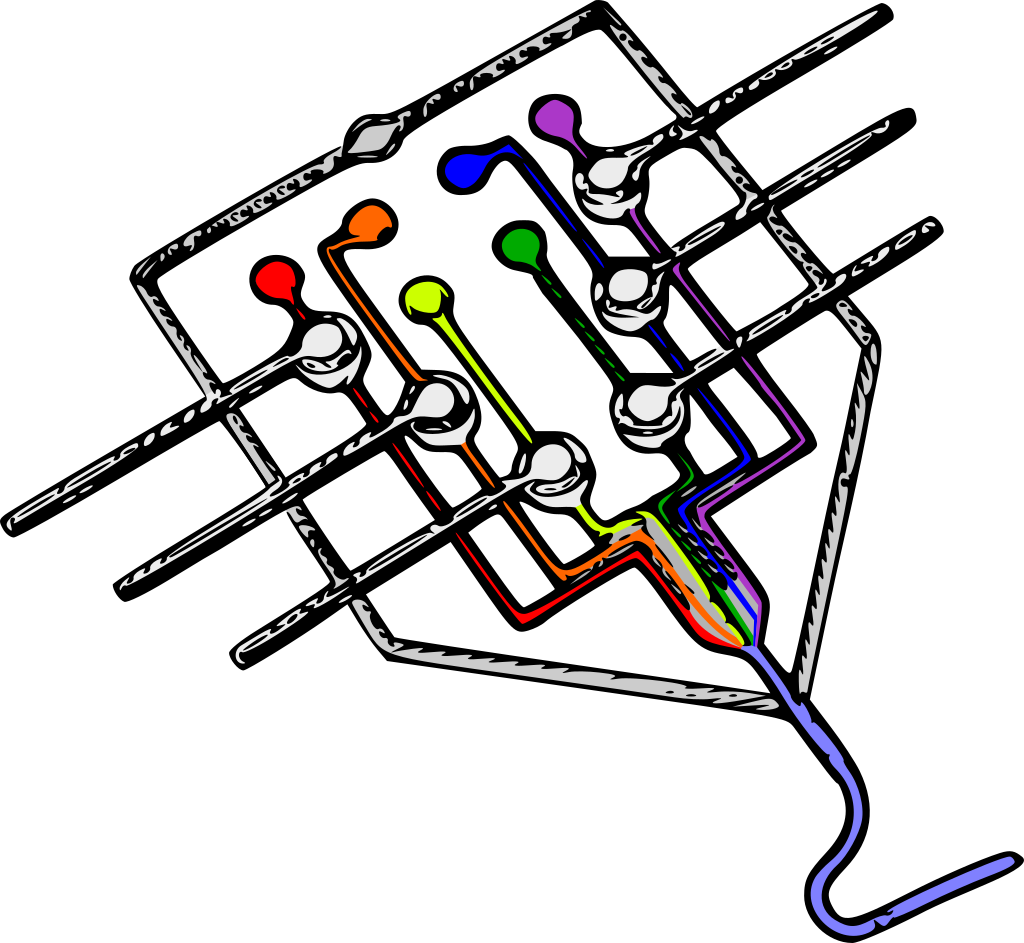
\includegraphics[scale=0.99]{./images/efb1d6af-4f1a-4c34-9726-b0015b59e112-uimg_microfluid_setup.png}}{}
\makeatother 
\caption{{Microfluidic device used by Kang et al.\unskip~\protect\cite{527120:13656548}}}
\label{f-c0beae2757bf}
\end{figure}
\egroup
Microfluidic techniques offer the possibility to embed several components into a single fiber, where each component can be released at different parts of the fiber. 



\subsection{Dispensing nozzle}Unlike traditional electrospinning, coaxial electrospinning (co-electrospinning) requires de implementation of a dual needle nozzle, where one needle is nested concentrically inside another needle, see Figure~\ref{f-4a5ffd16c3ab}\unskip~\cite{527120:13914792,527120:13914793}. The purpose of the co-electrospinning setup is to produce core/shell fibers, unlike mono axial electrospinning that yields monolithic fibers. Sun et al. \unskip~\cite{527120:13914312}. Addressed electrospinning setups, where both the core and shell are comprised by PEO (poly(ethylene oxide)) and for a PEO shell with a poly(dode-cylthiophene) core. Sun et al. state that co-electrospinning has the potential to extend the range of materials that can be used for electrospinning. The shell solution can be modified to make the core solution spunable. It was also discovered that non-spunable solutions can by implemented as shell solutions in conjunction with a spunable core solution. \unskip~\cite{527120:13914968}


\bgroup
%\fixFloatSize{./images/afe7da25-1366-4b1e-bf1a-0594eb2eaa88-uimg_nozzle.png}
\begin{figure}[!htbp]
\centering \makeatletter\IfFileExists{./images/afe7da25-1366-4b1e-bf1a-0594eb2eaa88-uimg_nozzle.png}{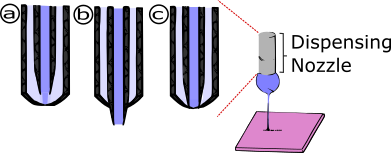
\includegraphics[scale=0.80]{./images/afe7da25-1366-4b1e-bf1a-0594eb2eaa88-uimg_nozzle.png}}{}
\makeatother 
\caption{{Needle configurations in coaxial electrospinning. (a) the outer needle encasing the inner; (b) the inner needle protruding from the outer; (c) both needles inline with each other;}}
\label{f-4a5ffd16c3ab}
\end{figure}
\egroup
Some advantages that co-electrospinning setups can break the polymer drop surface tension, initiating the jet burst from the spinneret nozzle. On the other hand, as the morphology and shape of the fibers depend on the polymer solution properties, the use of a co-axial nozzle allows the amendment of the material properties by producing bubbles, scaffolds and particles. \unskip~\cite{527120:13914748,527120:13914750}. As in conventional NFES, in co-electrospinning, the needle tip is connected to a high voltage power supply with a grounded collector.



\subsection{Polymer Reservoir (Polymer Melt \& Polymer Solution)}Electrospinning processes can be classified on the polymer reservoir type. As Brown et al. \unskip~\cite{527120:13445499} discussed, the polymer melt is equivalent to the polymer solution electrospinning (in place of a polymer solution a melt is used). The use of a polymer melt increases the complexity of the process, because the nozzle syringe and spinneret required to be heated to maintain the polymer in a liquid state. The fibers produced in melt spinning are typically found to have larger diameters than those from the polymer solutions due to the higher viscosity of a polymer melt than its solution. The apparatus used by Brown et al. \unskip~\cite{527120:13445499} is depicted in Figure~\ref{f-bfd139aecf8f}.


\bgroup
%\fixFloatSize{./images/9d06b4aa-134c-4fd6-bbf3-1ced4ac95046-uimg_metl_setup.png}
\begin{figure}[!htbp]
\centering \makeatletter\IfFileExists{./images/9d06b4aa-134c-4fd6-bbf3-1ced4ac95046-uimg_metl_setup.png}{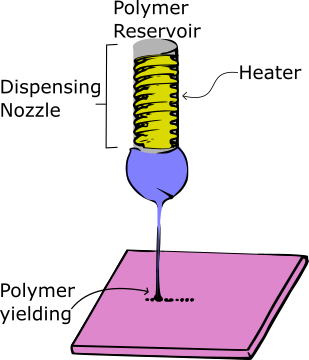
\includegraphics[scale=0.70]{./images/9d06b4aa-134c-4fd6-bbf3-1ced4ac95046-uimg_metl_setup.png}}{}
\makeatother 
\caption{{Typical Melt Electrospinning Setup}}
\label{f-bfd139aecf8f}
\end{figure}
\egroup
Despite the added complexity and thicker diameters, melt electrospinning  gets around the need to handle volatile solvents, making the process safer to be performed on larger scales. Furthermore, polymer melt reservoirs get rid of any solvent contamination.

The first report of a melt electrospun drug delivery system came from Nagy et al. \unskip~\cite{527120:13445555}, who prepared fibers by melt electrospinning of Eudragit EPO with carvedilol. The drug and polymer were melted and mixed to form a homogeneous solid mixture prior to spinning. The melt-spun fibers reached diameters of 5{\textendash}30 $\mu m $, compared to 300{\textendash}1000 $nm $ diameters produced from solution-spun fibers\unskip~\cite{527120:13445555}.

Balogh et al.'s work has been built on to blend plasticizes with the polymer Eudragit EPO and carvedilol active ingredient.\unskip~\cite{527120:13445752} The plasticizes Triacetin, Tween 80 and Polyethylene Glycol were investigated in order to reduce the melting point of the polymer-drug mixture. The temperature drop is desirable to minimize the occurring drug degradation.

Lian and Meng\unskip~\cite{527120:13445754} performed a comparison of poly(\ensuremath{\varepsilon }-caprolactone) (PCL) fibers fabricated by the melt and solution electrospinning techniques. They arrived to the conclusion that melt spinning is preferable when the polymer presents a low solubility. On the other hand the melt fibers were produced in a slower release rate. Gernot et al.\unskip~\cite{527120:13534159} demonstrated that submicron-size fibers are possible through melt electrospinning. In their effort, they achieved a precise deposition of PCL fibers with diameters of $817 \pm 165 nm $. 

In literature, melt electrospinning has less evidence than the solution approach. However, melt electrospinning arises to be as flexible as its solution counterpart in handling multiple polymers, as reported in McCann's work\unskip~\cite{527120:13534572}. Currently, the melt electrospinning setup is harder to determine and the lack of research on this technique explains its unexplored potential.



\subsection{Polymer Solution}In electrospinning, it is typically agreed that the diameter of the fibers increased with higher concentration due to greater viscosity which withstands stretching. In near field electrospinning, similar observations have been reported where concentration increases, fiber diameter increased\unskip~\cite{527120:11974306,527120:11974329}, seeFigure~\ref{f-d977f56a0782}.
\begin{table}[!htbp]
\caption{{Approximation process to estimate the critical polymer concentration. Several polymer concentrations are tried and the resulting jets are observed until a continuous stream is achieved.} }
\label{tw-be3662f66502}
\def\arraystretch{1}
\ignorespaces 
\centering 
\begin{tabularx}{\textwidth}{ll}
\hline Observation & Concentration Adjustment\\
\hline 
Dripping, no stream &
  Increase\\
Splitting small droplets &
  Increase slightly\\
Steady stream &
  No concentration adjustment\\
Splitting large globs &
  Decrease slightly\\
Nozzle clogging &
  Decrease\\
\hline 
\end{tabularx}\par 
\end{table}




\subsubsection{Polymers}The polymer selection is in function on the intended application. For example, a fast dissolving hydrophilic polymer such as poly(ethylene oxide) (PEO) is used for fast drug delivery systems. Otherwise, slow dissolving polymers such as poly($\varepsilon $-caprolactone) (PCL) or poly(lactic-co-glycolic acid) (PLGA) are implemented. \unskip~\cite{527120:13082763}

The polymer molecular weight along with the polymer concentration and solvent selection have a direct effect on the solution viscosity, conductivity and surface tension, hence the solution behavior in the electrospinning process. The spunable viscosity range varies with the polymer and solvent. 

Solutions with low viscosity are prone to insufficient polymer chain entanglements to produce fibers.\unskip~\cite{527120:13082763} On the other hand, if the solution is too viscous, then the surface tension cannot easily be overcome by the electric field. In both cases, the result can be droplets or particles forming rather than fibers as described inTable~\ref{tw-be3662f66502}.



\subsubsection{Solvents}The solvent used must be capable of dissolving the polymer of interest at an appropriate concentration to form fibers, and must posses a suitable volatility. A low-volatility solvent like water may fail to evaporate completely over the distance between the spinneret and the collector. When the fibers form, they will hence contain residual water owing to this incomplete evaporation. The residue solvent will subsequently evaporate from the fibers upon storage, resulting in ribbon-like (flattened) fibers, wrinkles on the fiber surface or fused fibers. On the other hand, a high-volatility solvent may evaporate very quickly, leading to larger fiber diameters (less time for elongation before solidification) and clogging of the spinneret (due to drying of the liquid at the spinneret before jetting, or drying of the Taylor cone during jetting). Solvents commonly used for electrospinning include ethanol, chloroform, trichloroethane and hexafluoroisopropanol\unskip~\cite{527120:12073495,527120:16887323,527120:16887324}.

Mixtures of miscible solvents can be used to ensure that sufficient polymer can be dissolved to give a solution of appropriate viscosity and volatility with suitable dielectric constant range to allow fiber formation. However, care must be taken because using a mixture of solvents with very different volatilities can result in porous fiber structures. As reported by Katsogiannis et al. for organic solvent mixtures with dimethyl sulfoxide (DMSO).\unskip~\cite{527120:13082766} DMSO evaporates much more slowly than the organic solvents used, which results in its incorporation into the fibers. The DMSO will eventually evaporate, yielding porous fibers.

It is also important to take into account the surface tension of the solution. Solvents with very high surface tensions (e.g. water) can result in instability arising during the spinning process, and a broad range of fiber diameters in the products. If necessary, a surfactant can be added to reduce the surface tension, but this will be incorporated into the fibers produced.
    
\section{Properties that Improve Accuracy of Nano-Fiber Deposition}
Near-field electrospinning is considered to be an outstanding technique to fabricate polymer fibers with spatial control and it has suffered several modifications to improve the precision and accuracy of the fiber deposition. This paper intents to collect the NFES variants of electrospunable polymer solutions with spatial control in recent research. Table S1 is a collection of the relevant NFES process parameters and achieved fiber morphology.

Some differences have been discovered between LV-NFES and conventional NFES. Low voltage near field electrospinning produces thinner fibers with lower voltages; as shown inFigure~\ref{f-59ed68f95344}. Moreover, when implementing a moving stage, the fibers are affected by the mechanical stretching. Bisht et al. and Chang et al. \unskip~\cite{527120:11973130,527120:11974313} reported that thinner diameters are yield with the increase of the x-y stage velocity, and larger diameters by decreasing the stage velocity.

Bisht and Chang's work \unskip~\cite{527120:11973130,527120:11974313} reports a controlled technique to fabricate polymeric nano fibers in a continuous manner, using a low voltage setup. Their purpose is to find a workaround to the drawbacks of traditional NFES by using a superelastic polymer precursor, which allow continuous patterning without breaking. In low voltage near-field electrospinning (LV NFES), a visco-elastic polymer is used to allow continuous spinning at about 200$V $.

Kim et al. \unskip~\cite{527120:11974313} experimented with a NFES variation where the fiber deposition is guided by conductive rails, see Figure~\ref{f-927e96fb5537}. As stated by the authors, the induced electric field is enhanced by the conductive pattern, which allows the fibers to follow the desired deposition path. As the fibers are prone to follow the conductive pattern, additional fibers can be stacked on each other. The stacking process was successfully achieved in high electric field conditions at: 750$\mu m $ substrate to collector distance, and a 600 $\mu m $ needle to rail (offset) distance, see Figure~\ref{f-927e96fb5537}.


\bgroup
%\fixFloatSize{./images/0fd23deb-7631-4b09-8641-69fc6ac8a6b5-ukim_00.png}
\begin{figure*}[!htbp]
\centering \makeatletter\IfFileExists{./images/0fd23deb-7631-4b09-8641-69fc6ac8a6b5-ukim_00.png}{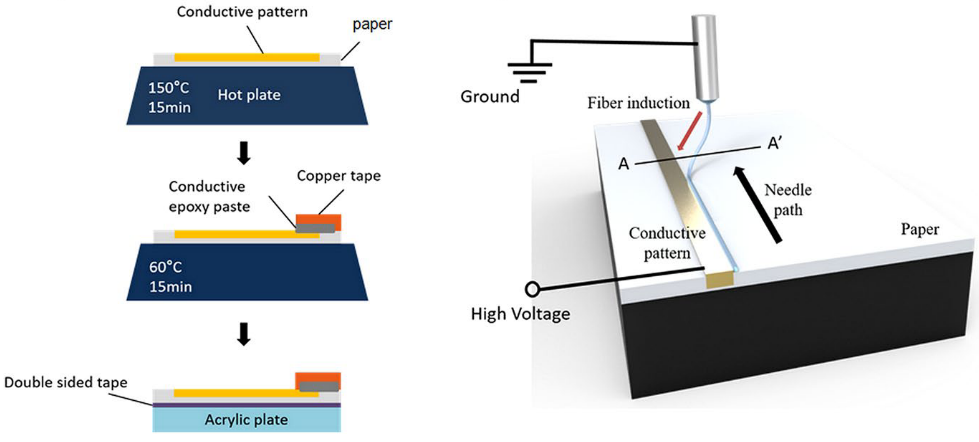
\includegraphics[scale=0.70]{./images/0fd23deb-7631-4b09-8641-69fc6ac8a6b5-ukim_00.png}}{}
\makeatother 
\caption{{NFES setup for controlled fiber deposition on pre-patterned conductive electrodes. \unskip~\protect\cite{527120:11974313}}}
\label{f-927e96fb5537}
\end{figure*}
\egroup
Gupta et al.\unskip~\cite{527120:11974310} introduced a new technique to fabricate polymer scaffolds for tissue engineering applications and organ development. As described by Gupta et al.\unskip~\cite{527120:11974310}, the fiber deposition equipment is comprised by a stainless steel needle with a internal diameter of 750 $\mu m $ , connected to a high voltage power supply of up to 30 $k V $ with a deposition rate of about $\geq 1 \mu L min^{-1} $. The setup was embedded to a motorized collector capable of controlled programmable motions, see Figure~\ref{f-74de1f00848b}. The proposed technique was able to produce fibers of $150 \mu m $ in diameter with pre-designed patterns.


\bgroup
%\fixFloatSize{./images/fa274bb7-a79d-48ae-9349-953df62c0094-ugupta_00.png}
\begin{figure}[!htbp]
\centering \makeatletter\IfFileExists{./images/fa274bb7-a79d-48ae-9349-953df62c0094-ugupta_00.png}{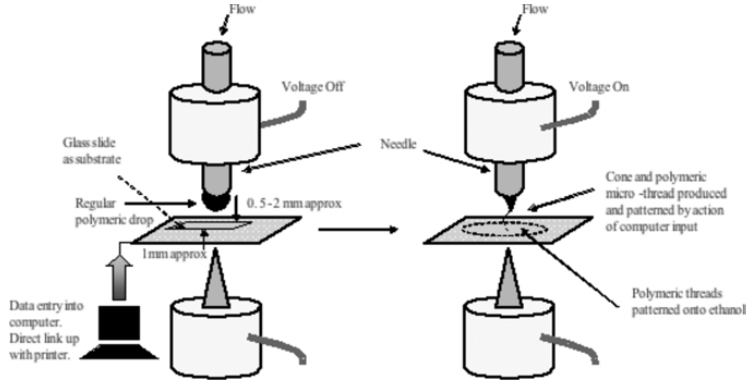
\includegraphics[scale=0.60]{./images/fa274bb7-a79d-48ae-9349-953df62c0094-ugupta_00.png}}{}
\makeatother 
\caption{{Schematic illustration of the electrohydrodynamic process. \unskip~\protect\cite{527120:11974310}}}
\label{f-74de1f00848b}
\end{figure}
\egroup
Wang, et al., Huang, et al., and Chen, et al. \unskip~\cite{527120:11974322,527120:11974323,527120:11974324} experimented with several multi-nozzle near-field electrospinning of aligned nano fibers. The multi nozzle NFES apparatus is similar to the one used in conventional NFES with some modifications to the needle nozzle, see Figure \ref{f-4a1a1f58a423}. The authors implemented similar NFES setups where the installed linear array of nozzles is supplied with a constant flow rate of solution.

\bgroup
%\fixFloatSize{./images/cd8e0617-d4d9-479b-a99b-a466cd21483c-uwang_01.png}
\begin{figure}[!htbp]
\centering \makeatletter\IfFileExists{./images/cd8e0617-d4d9-479b-a99b-a466cd21483c-uwang_01.png}{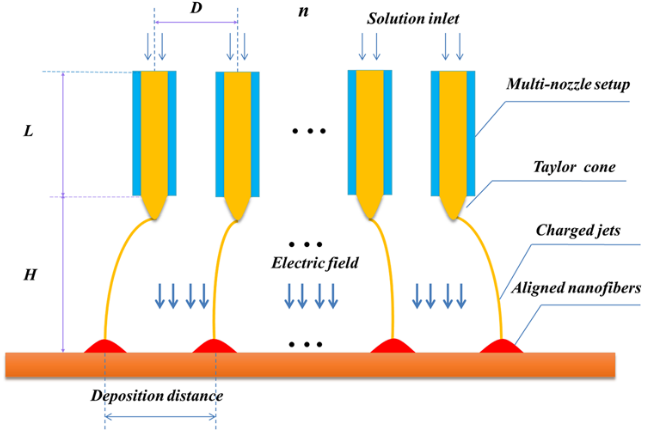
\includegraphics[scale=0.70]{./images/cd8e0617-d4d9-479b-a99b-a466cd21483c-uwang_01.png}}{}
\makeatother 
\caption{{The geometry distribution of linear array multi-nozzle system \unskip~\protect\cite{527120:11974323}}}
\label{f-4a1a1f58a423}
\end{figure}
\egroup
The authors came to the conclusion that the distance between the deposited fibers increase with the increase of the needle-to-collector distance, as the influence of the applied voltage dissipates.

Huang, et al.\unskip~\cite{527120:11974311} studied the mechanoelectrospinning (MES) technique for the fabrication of nano fibers. The MES technique tries to improve deposition accuracy by the introduction of a mechanical drawing force. The MES is predominantly controlled by the collector stage velocity, the nozzle-to-collector distance, and the applied voltage. The authors believe that MES can compete as a low-cost, high precision fabrication of electronics and enable the direct writing of structures for nano scale lithography. Figure~\ref{f-7587d8081ccc} shows the polymer jet behavior when a mechanical force is implemented within the NFES process.


\bgroup
%\fixFloatSize{./images/db7d3b35-fe08-422f-afe4-78e0133b489b-uhuang_00.png}
\begin{figure}[!htbp]
\centering \makeatletter\IfFileExists{./images/db7d3b35-fe08-422f-afe4-78e0133b489b-uhuang_00.png}{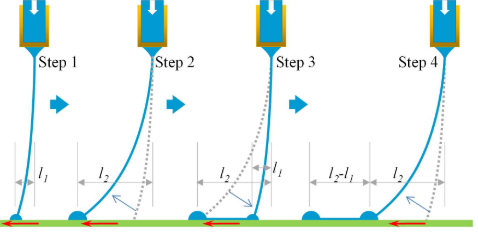
\includegraphics[scale=0.90]{./images/db7d3b35-fe08-422f-afe4-78e0133b489b-uhuang_00.png}}{}
\makeatother 
\caption{{schematic diagram of leap direct-writing: the ink first accumulates at contact point and then gets stretched by mechanical drawing force. At a critical distance, the ink leaps to the next contact point, and gets stretched again \unskip~\protect\cite{527120:11974311}}}
\label{f-7587d8081ccc}
\end{figure}
\egroup
Micro and nano fibers have been written using AC pulse-modulated electrospinning by Bu et al. with polyehtylene terephthalate (PET) as substrate\unskip~\cite{527120:11974304}. The AC electrical field influences the electrospinning jet. The alternate current tends to decrease the repulsive electrical force allowing a stable straight jet between the dispensing nozzle and the insulating PET substrate. Bu et al. varied the stage velocity; faster stage velocities enable the deposition of straighter fibers\unskip~\cite{527120:11974304}.

 A mechano-electrospinning technique was presented by Nagle et al.\unskip~\cite{527120:12033656}. With the implementation of a mechanical drawing force, a higher resolution nano fibrous pattern can be produced with lower voltages as the Taylor cone becomes more stable. Nagle et al. studied PEO fibers at different nozzle to collector distances. Evidence suggest that better patterning accuracy increases with increasing nozzle to collector distance as the solution is effectively dried\unskip~\cite{527120:12033656}. Near field mechano-electrospinning enables the collection of non woven fibers over large areas.


\bgroup
%\fixFloatSize{./images/43f61edd-73cd-4222-830e-3333f92934e9-uimg_nfesvariants.png}
\begin{figure}[!htbp]
\centering \makeatletter\IfFileExists{./images/43f61edd-73cd-4222-830e-3333f92934e9-uimg_nfesvariants.png}{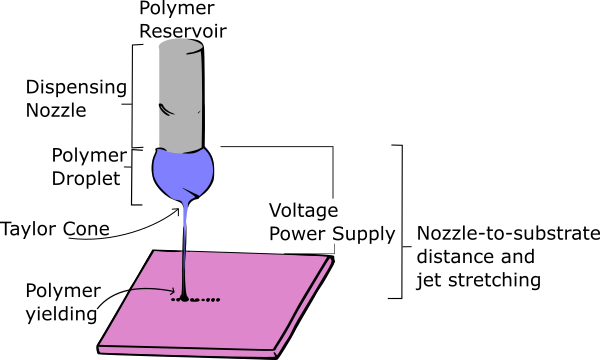
\includegraphics[scale=0.65]{./images/43f61edd-73cd-4222-830e-3333f92934e9-uimg_nfesvariants.png}}{}
\makeatother 
\caption{{Near-Field ES Process Parameters}}
\label{f-3629d3a3f9cf}
\end{figure}
\egroup
To spin nano fibers at close distances, the initial diameter of the jet is required to be as small as possible since stretching of the thread is limited. Kameoka et al.\unskip~\cite{527120:12321556} demonstrated that a small initial spinning radius can be achieved using an atomic force microscope tip with a small polymer solution drop at the tip.

Near-field electrospinning, has exhibited to be capable fabricate nano fibers and nano fiber patterns \unskip~\cite{527120:11974321}. Nevertheless, having a small polymer solution drop at the nozzle tip limits the length of the fibers that can be fabricated in a continuous manner. Using a spinneret with a reservoir (e.g. syringe) of solution generally produces fibers with diameter of a few micrometers \unskip~\cite{527120:11974310,527120:11974326}, since it creates a limit to which the nozzle inner diameter can be reduced to allow the solution to flow through. As shown inFigure~\ref{f-51afaccaf109}, the implementation of thicker needle nozzles translate into an increase of the resulted fiber diameter

Coppola et al.\unskip~\cite{527120:11974307} have showed a NFES variant that allows polymer nano fibers to be deposited directly from a polymer drop, averting the issue of nozzle clogging. The fibers are also prone soaking after deposition thus giving the fibers a semi-circular cross-section as depicted in Xue et al.'s\unskip~\cite{527120:11974326} work.



\subsection{Nozzle spinneret}The thinnest nozzles in literature so far are about $50 nm $ in diameter, by Chang et al.\unskip~\cite{527120:11974306} who used a  $100 \mu m $ inner diameter needle tip to electrospin poly(ethylene oxide) (PEO). Camillo et al.\unskip~\cite{527120:12322072} used a micro-diameter tip Tungsten spinneret in a 26G needle to electrospin co-polymer, poly[2-methoxy-5-(2-ethylhexyloxy)-1,4-phenylenevinylene] (MEH-PPV) with poly(ethylene oxide) (PEO). The nozzle most commonly comprises a simple narrow-bore, blunt-end metal needle. The diameter of the needle can vary, but most commonly researches work with internal diameters below 1 $mm $ . This translates to needles of gauge 18{\textendash}22. In general, this simple spinneret design can be used to achieve successful spinning. A blunt-end rather than a tapered-end for the needle exit is important as the size distribution of the products increase with an increase in needle tip angle. However, it should be noted that there will be some interactions between the solvent and polymer molecules in the solution and the metal surface of the spinneret. There will exist some attractive forces between the polar groups in the polymer and the electro-positive metal surface, which can act counter to the drawing force of the electric field and can pull the polymer solution back into the spinneret. It has been found that coating the spinneret exterior in a non-conductive and non-stick polymer such as Teflon or epoxy coating can reduce these interactions.\unskip~\cite{527120:13082768,527120:13082811} As a result, the electrical energy can be more efficiently used to elongate and narrow the polymer jet, and narrower fibers can be produced. In addition, strong attractive forces between the polymer jet and the metal spinneret can result in fibers becoming attracted to the needle, leading to lower yields and potentially to blocking of the exit orifice.



\subsection{Applied Voltage}In recent literature, near field electrospinning has been studied to reduce the fiber diameter and to improve the fiber deposition accuracy. Madou et al.\unskip~\cite{527120:11973130} and Chang et al.\unskip~\cite{527120:11974306} came to the conclusion higher voltages yield thicker micro-fibers with a loss in jet stability. This relationship between the applied voltage and resulting fiber diameter is influenced by other variables such as nozzle-to-substrate distance and solution deposition rate. For instance, if a high voltage is applied at a low deposition rate then electrospraying is achieved, meaning the formation of several non-continuous fibers. The applied voltage shall be sufficient to break the surface tension and initiate the jet, but low enough to avoid multiple jets at the nozzle tip.

Madou et al.\unskip~\cite{527120:11973130} achieved the fabrication of thinner fibers with spatial control by reducing the applied voltage to 200-600 $V $  at a nozzle-to-substrate distance of 0.5-1 $mm $. The low voltage setting does not create enough charge to break the polymer solution surface tension to initiate the electrospinning process.

Madou et al.\unskip~\cite{527120:11973130} and Chang et al.\unskip~\cite{527120:11974306} initiated the electrospun fibers by mechanically pull the polymer solution at the nozzle tip using a micro-probe tip. Chang and coworkers reduced the applied voltage from 1.5 $kV $ to 600 $V $ with a nozzle-to-substrate distance of 500 $\mu m $ to yield a fiber diameter between 3 $\mu m $  and 50 $nm $ . With an applied voltage of 200 $V $ and a nozzle-to-substrate distance of 1 $mm $.

In near-field electrospinning, the applied voltage has an impact on the produced fiber morphology. For instance, a voltage higher or lower to the optimum voltage will translate into an increase in fiber diameter. Song et al.\unskip~\cite{527120:11974320} demonstrated that a decrease in voltage from 400 to 500 $V $ can reduce the fiber diameter from 160 to about 60 $nm $with a nozzle-to-substrate distance of 20 $\mu m $. A workaround to break the polymer solution surface tension is to initialize the NFES process with a higher voltage and then lower the voltage once the jet is created. Huang et al.\unskip~\cite{527120:11974311} implemented the previous and yield ordered fibers with a distance between adjacent fibers of 50 $\mu m $.



\subsection{Nozzle-to-substrate distance}
\bgroup
%\fixFloatSize{./images/4cc65220-1457-4d0d-bb04-9b1c8138aa96-uffes_vs_nfes.png}
\begin{figure*}[!htbp]
\centering \makeatletter\IfFileExists{./images/4cc65220-1457-4d0d-bb04-9b1c8138aa96-uffes_vs_nfes.png}{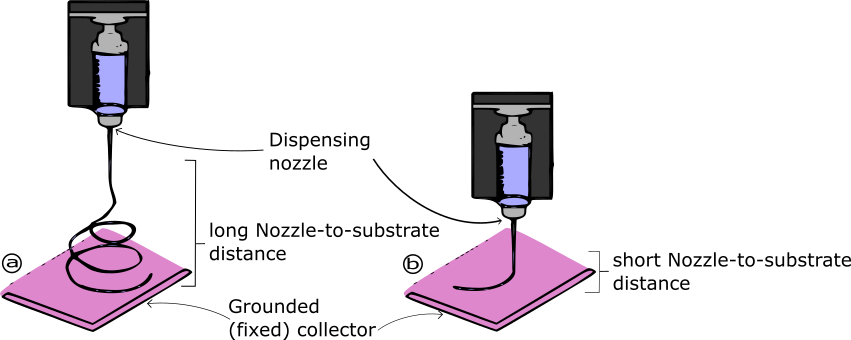
\includegraphics[scale=0.65]{./images/4cc65220-1457-4d0d-bb04-9b1c8138aa96-uffes_vs_nfes.png}}{}
\makeatother 
\caption{{a) Typical Far-field Electrospinning (FFES) Setup. b) Typical Near-field Electrospinning (NFES) Setup.}}
\label{f-c34559531e3e}
\end{figure*}
\egroup
Figure~\ref{f-c34559531e3e}.a, depicts the typical setup for the conventional far-field electrospinning (FFES). As stated in previous sections, the precursor polymer droplet becomes charged with the employment of an electric field between the polymer solution and the collector\unskip~\cite{527120:14135125}. When the polymer solution surface tension is overcome by the electric field potential difference a jet is formed, starting the electrospinning process. The electrospinning process can be break down into two steps: i) first the jet travels in a straight line, and ii) the jet begins to curl due to bending and whipping instabilities \unskip~\cite{527120:13444381,527120:14135543}. The fiber spatial control in far-field electrospinning is limited due to the instabilities, inhibiting the precise deposition of fibers.

In the intent to achieve controlled fiber deposition, Sun et al. \unskip~\cite{527120:11974321} reported an electrospinning variation known as near-field electrospinning (NFES),Figure~\ref{f-c34559531e3e}.b, describes the near-field electrospinning setup, where the distance between the dispensing nozzle and the collector is reduced to write fibers while the jet travels in a straight line. Moreover, some mechanical influence is required to deposit fibers precisely. The mechanical force is introduced by moving collector. If the polymer solution jet speed is faster than the speed of the moving collector, the written fiber will curl; on the other hand, if the collector moves faster than the polymer jet, the fiber will gradually diminish \unskip~\cite{527120:11974327,527120:11974326}. Currently, due to the lack of theoretical models, the near-field electrospinning process parameters (such as the collector speed) are typically tuned by experience and experimentation only.

The main difference between NFES and FFES is the distance between the needle and the collector which is higher in FFES (about 10 cm) compared to NFES which ranges in the mm scale. The short distance allow the production of well aligned fibers within particular designs. In NFES, the fiber morphology can be altered by the control of the distance between the nozzle and the substrate (collector). With the decrease of the nozzle-to-substrate distance, the electric field strength increases; however it can cause incomplete solvent volatilisation and possible short circuits between the collector and the nozzle tip.

An optimal nozzle-to-substrate distance shall be defined to ensure the fabrication of dry continuous fibers. If the solvent is not well evaporated, the produced fibers are prone to defects; on the other hand if solidification happens too fast, the solids can block the spinneret which can prevent a continuous fiber yield. Furthermore, the polymer jet will discharge itself as soon as possible, therefore long distances can result in low yields.



\subsection{Substrate}Due to the close distance between the grounded substrate and the charged spinneret in NFES, the set up is prone to electrical shorts. In NFES, when a short circuit takes place, the electrospinning process is interrupted resulting in the fabrication of discontinuous fibers. Two workarounds to avoid electrical shorts is to lower the applied voltage and to use less conductive substrates \unskip~\cite{527120:11974315,527120:12322289}.

Liu et al.\unskip~\cite{527120:11974315} discovered that the fiber alignment is improved by using a glass-cooper foil substrate, however the well aligned fibers are spoiled after prolonged depositions due to residual charges. Additionally, the effect of residual charges is amplified with the used collector substrate contains a conductive layer and a non-conductive layer\unskip~\cite{527120:11974315}.

On the other hand, Choi et al.\unskip~\cite{527120:12322289} implemented a hydrophilic substrate to deposit the fibers with plasma treatment to increase the conductivity of selected areas. NFES was carried put with precise deposition as the fibers were placed as per the desired design within the hydrophilic substrate.

\section{Data collection of NFES fiber morphology and process parameters}

Near-field electrospinning process parameters and achieved fiber morphology data was collected into a single database with the purpose to analyze the data and find correlations between the process parameters and the obtained fiber morphology after a NFES process. The alalysis comprises from the first reported NFES apparatus built in 2003 by J. Kameoka et al. \cite{Kameoka2003a} to recent studies conducted in 2020. \cite{
  Yang2019,Fattahi2017,Shin2019,Wang2015,Parajuli2016,Zheng2010,Fuh2011,Dalton2015,
  Ru2014,Xue2014,Wang2017,Xu2014,Liu2013,Pan2014,Canton2014,Chakraborty2009,Gupta2007,
  He2018,Zhou2011,Chen2013,Williams2018,Choi2017,Pan2019,Lei2015,Lim2019,Park2020,
  Fuh2012,Flores2017,Chang2010,Xu2019,Zhang2019,Shin2018,Fuh2015,Nagle2019,Zheng2012,
  Kameoka2003a,Liu2014,E.King2019,Hochleitner2017,Madou2011,Jiang2018,Husain2016,
  ElectrospinTech2015,Brown2011,Kolan2018,Chang2011,Beachley2011,Camillo2013,Kameoka2003,
  Bu2012,Lee2012,Huang2015,Coppola2020,CisquellaSerra2019,Ruggieri2013,Hochleitner2014,
  Zhu2016,Brown2014,Chang2008,Sonntag2020,Kim2018,Deng2020,Han2019,George2020,Sun2006a,
  Pan2015,Shen2016,Strauss2019,Fuh2013,Sarkar2007,You2017,Wang2018a,Zheng2014,Song2015,
  GaofengZheng2010,Liu2015a,Min2013,Luo2016,Yousefi2019,Cardenas2017,Coppola2014} The data collection process was divided in three procedures depending on the format of the available information, as follows:

\begin{enumerate}
\item Case 1 : data is collected as is from literature. This procedure was implemented when the data is listed within tables and/or as text format.
\item Case 2 : data is only presented in a figure as plots.
\item Case 3 : data is not available in text format or plots, however Scanning Electron Microscopy Images (SEM) images are reported from the obtained fibers.
\end{enumerate}

\subsection{Image Analysis - Data extraction from plots}

Most numerical data of NFES process parameters and fiber diameters is available only in the form of plots. The reported figures provide a visual relationship between the variables of interest, however recovering the numerical values of the data is a tedious process prone to errors. To avoid mistakes and accelerate the collection data from plots, \href{https://github.com/ankitrohatgi/WebPlotDigitizer}{WebPlotDigitizer} was used. WebPlotDigitizer is a HTML5 tool that facilitates accurate data extraction with ease of use. Figure \ref{fig:screenshotWebPlotDigitizer} is a screenshot of the software in use.

\begin{figure}[th]
\centering
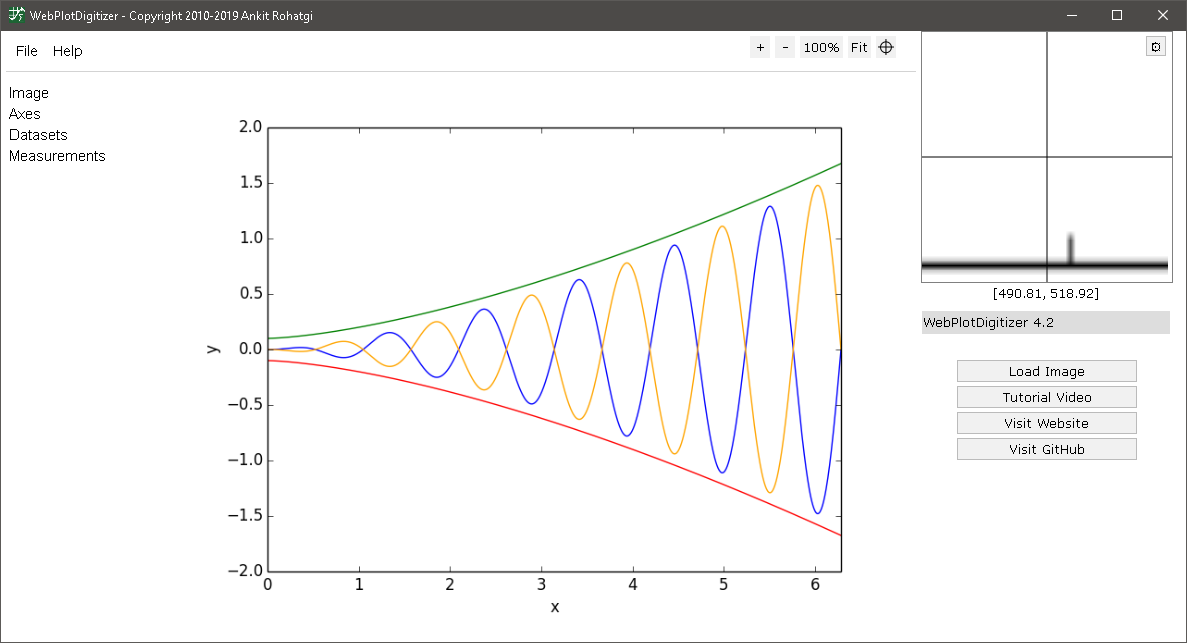
\includegraphics[scale=0.45]{./Figures/screenshotWebPlotDigitizer.png}
\decoRule
\caption[WebPlotDigitizer home-screen]{Open session of WebPlotDigitizer \href{https://github.com/ankitrohatgi/WebPlotDigitizer}{github.com}}
\label{fig:screenshotWebPlotDigitizer}
\end{figure}

\subsection{Image Analysis - Data extraction from Scanning Electron Microscopy Images}

Scanning Electron Microscopy Images (SEM) images contain information in a two-dimensional grid that can be extracted using point and line counting techniques, however this can be a laborious process for a large number of images. To decrease the complex and lavorious aspect of the counting process, a \emph{Python} script was developed to measure fiber diameters from the available SEM images. As shown in Figure \ref{fig:imageAnalysisAlgorithm}, the image analysis algorithm follows three main steps: pre-processing, segmentation, object detection, and data processing.

\begin{figure}[!th]
\centering
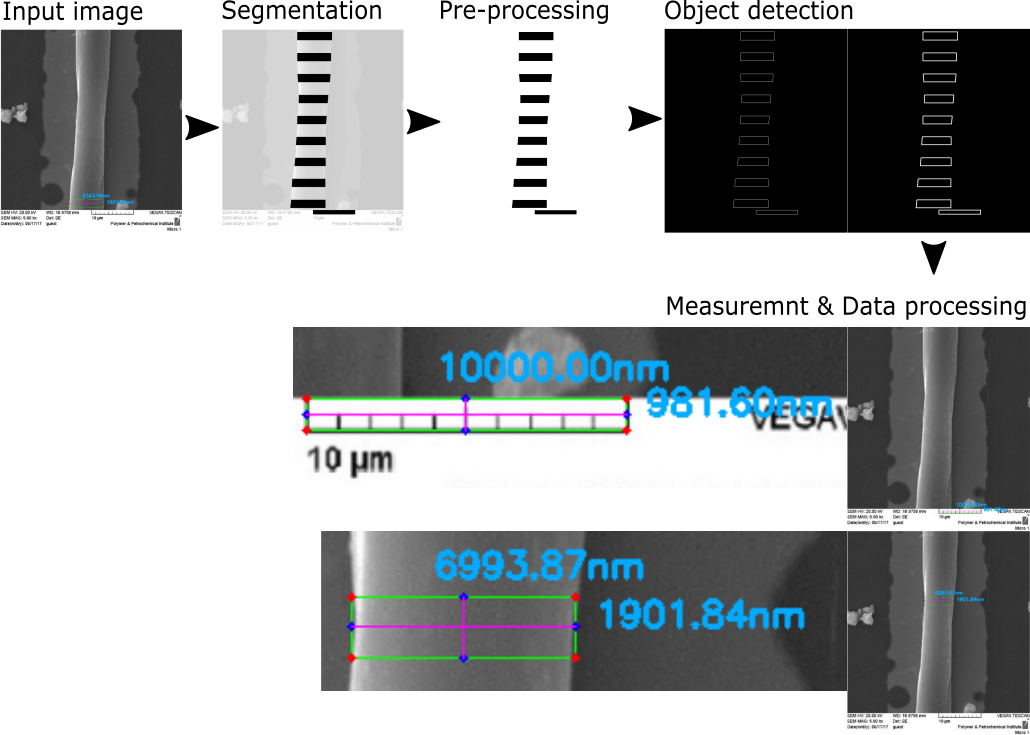
\includegraphics[scale=0.50]{./Figures/imageAnalysisAlgorithm.png}
\decoRule
\caption[Image Analysis Algorithm to Measure Fiber Diameters from SEM images]{Image Analysis Algorithm to Measure Fiber Diameters from SEM images. Ilustration uses Yousefi et al.'s work as an example. \cite{Yousefi2019}}
\label{fig:imageAnalysisAlgorithm}
\end{figure}

The adopted image analysis was implemented with the \emph{Python} package \emph{OpenCV}. First a segmentation procedure is executed over an input image to delimit the objects to be measured (fiber sections and scale bar). The segmentation step is the only step needed to be done manually in a image processing software, in this case \emph{Inkscape} was used. Next, the segmented image is passed to the \emph{Pyhton} script, which will convert its input image into a binary image. A binary image is a black and white image (with no gray scale) that ease the detection of the object edges as the color intensity change between the objects and the background is well defined. Once the binary image is computed, the \emph{Canny} edge detection algorithm is executed. Once the edges are well defined, a the image is dilated to make the edges more visible. The final step before measurement, the \emph{OpenCV} \emph{findContours} function is called to store the objects in memory. The first object to be measured is the scale bar as this is needed as a reference to convert the pixel counts to a metric unit. Finally, the objects are located within the image with four edge points, and the reference object is used to compute the metric length as the ratio of counted pixels between two edge points and the scale bar dimension in meters.

Measurements were validaded with Camillo's, Gupta's, Jiang's, Min's, Sun's, Wang's, and Xue's \cite{Camillo2013, Gupta2007, Jiang2018, Min2013, Sun2006a, Wang2015, Xue2014} results as those authors reported both, a SEM image and the measured fiber diameter. For instance, Figure \ref{fig:imageAnalysisToolValidation} shows in white the reported diameters by Min and in blue the diameters measured by the \emph{Python script}. The measurement error of the developed script is about $3.2\%$ in avg. It is considerable to mention that the reported measurement error is mainly contributed to the fact that most fibers are not of the same diameter along the fiber length. In most cases, measurements at the end of the fibers are thicker than the ones measured u¿in the center.

\begin{figure}[!th]
\centering
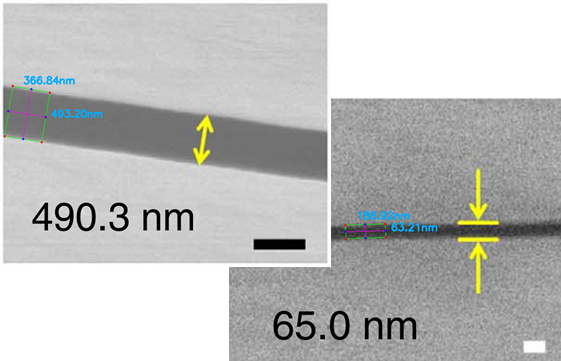
\includegraphics[scale=0.8]{./Figures/imageAnalysisToolValidation.png}
\decoRule
\caption[Validation of the developed image analysis meassurement tool]{{Validation of the developed image analysis meassurement tool. SEM images of Min's work are used as an example. \cite{Min2013}}}
\label{fig:imageAnalysisToolValidation}
\end{figure}

\section{Discussion \& NFES Challenges}

Helix electrodynamic printing (HE-printing) was presented by Duan et al. \unskip~\cite{527120:11974308} with the intention of depositing aligned fibers. The authors fabricated a stretchable piezoelectric device using micro and nano fibers to demonstrate the possible applications of HE-printing for electronics manufacturing. Duan et al. concluded that the fiber morphology is mainly driven by: the stage velocity, the applied voltage, and the nozzle-to-collector distance.

\begin{figure}[!th]
\centering
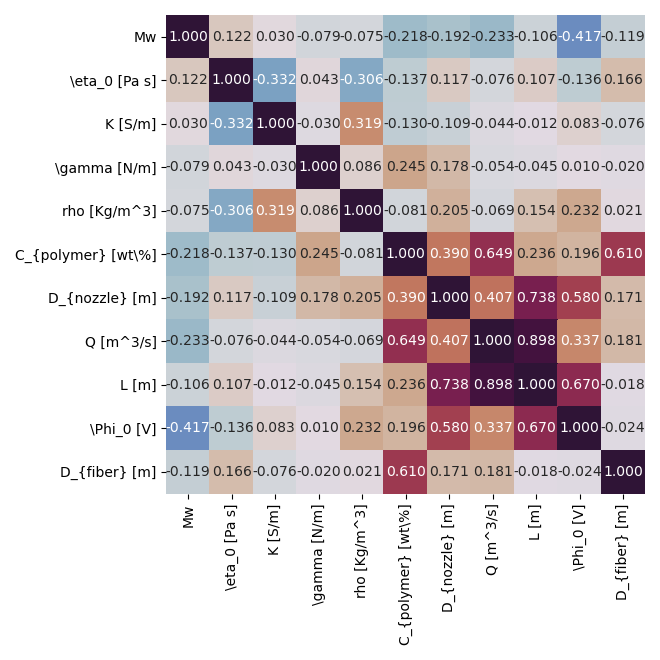
\includegraphics[width=\textwidth]{./Figures/plt_corMat.png}
\decoRule
\caption[NFES correlation matrix of process parameters and fiber morphology]{{Correlation matrix comprised by the NFES data from recent literature. 
\cite{
  Yang2019,Fattahi2017,Shin2019,Wang2015,Parajuli2016,Zheng2010,Fuh2011,Dalton2015,
  Ru2014,Xue2014,Wang2017,Xu2014,Liu2013,Pan2014,Canton2014,Chakraborty2009,Gupta2007,
  He2018,Zhou2011,Chen2013,Williams2018,Choi2017,Pan2019,Lei2015,Lim2019,Park2020,
  Fuh2012,Flores2017,Chang2010,Xu2019,Zhang2019,Shin2018,Fuh2015,Nagle2019,Zheng2012,
  Kameoka2003a,Liu2014,E.King2019,Hochleitner2017,Madou2011,Jiang2018,Husain2016,
  ElectrospinTech2015,Brown2011,Kolan2018,Chang2011,Beachley2011,Camillo2013,Kameoka2003,
  Bu2012,Lee2012,Huang2015,Coppola2020,CisquellaSerra2019,Ruggieri2013,Hochleitner2014,
  Zhu2016,Brown2014,Chang2008,Sonntag2020,Kim2018,Deng2020,Han2019,George2020,Sun2006a,
  Pan2015,Shen2016,Strauss2019,Fuh2013,Sarkar2007,You2017,Wang2018a,Zheng2014,Song2015,
  GaofengZheng2010,Liu2015a,Min2013,Luo2016,Yousefi2019,Cardenas2017,Coppola2014} Fiber diameter is highly correlated with polymer solution concentration and slightly correlated with solution flow rate, zero-shear viscosity and nozzle diameter.}}
\label{fig:plt_corMat}
\end{figure}

Figures \ref{fig:plt_Cpolymerwt_vs_Dfiberm}, \ref{fig:plt_Dnozzlem_vs_Dfiberm}, \ref{fig:plt_Lm_vs_Dfiberm}, \ref{fig:plt_Phi0V_vs_Dfiberm}, \ref{fig:plt_Qm3s_vs_Dfiberm} and \ref{fig:plt_vstagems_vs_Dfiberm} are scatter plots that depict the relationship of various process parameters (polymer concentration $C_{polymer}$, nozzle inner diameter $D_{nozzle}$, NFES working distance $L$, NFES applied voltage $\Phi_0$, flow rate $Q$, and stage velocity $v_{stage}$) with the final fiber diameter $D_{fiber}$. In a generalized summary, these figures suggest that thin fibers are produced with the implementation of low polymer concentrations, small nozzle diameters, short working distances, low applied voltages, low flow rates, and high stage xy velocities. Moreover, based on the degree of dispersion of the data points, polymer concentration $C_{polymer}$ is the most reliable process parameter to describe and predict the behavior of the fiber diameter, as most of the data can be grouped in a single cluster. Unlike $C_{polymer}$ in Figure \ref{fig:plt_Cpolymerwt_vs_Dfiberm}, various data clusters can be identified within the other scatter plots. For instance, Song's results \cite{Song2015} deviate from the main cluster in Figures \ref{fig:plt_Dnozzlem_vs_Dfiberm}, \ref{fig:plt_Lm_vs_Dfiberm}, \ref{fig:plt_Phi0V_vs_Dfiberm}, and \ref{fig:plt_vstagems_vs_Dfiberm}, this may be because Song et al. used Au/Pd coated glass capillary nozzles instead of the traditional stainless steel precision tips. However in the $C_{polymer}$ vs. $D_{fiber}$ figure, Song's results fit within the main cluster.

\begin{figure}[!th]
\centering
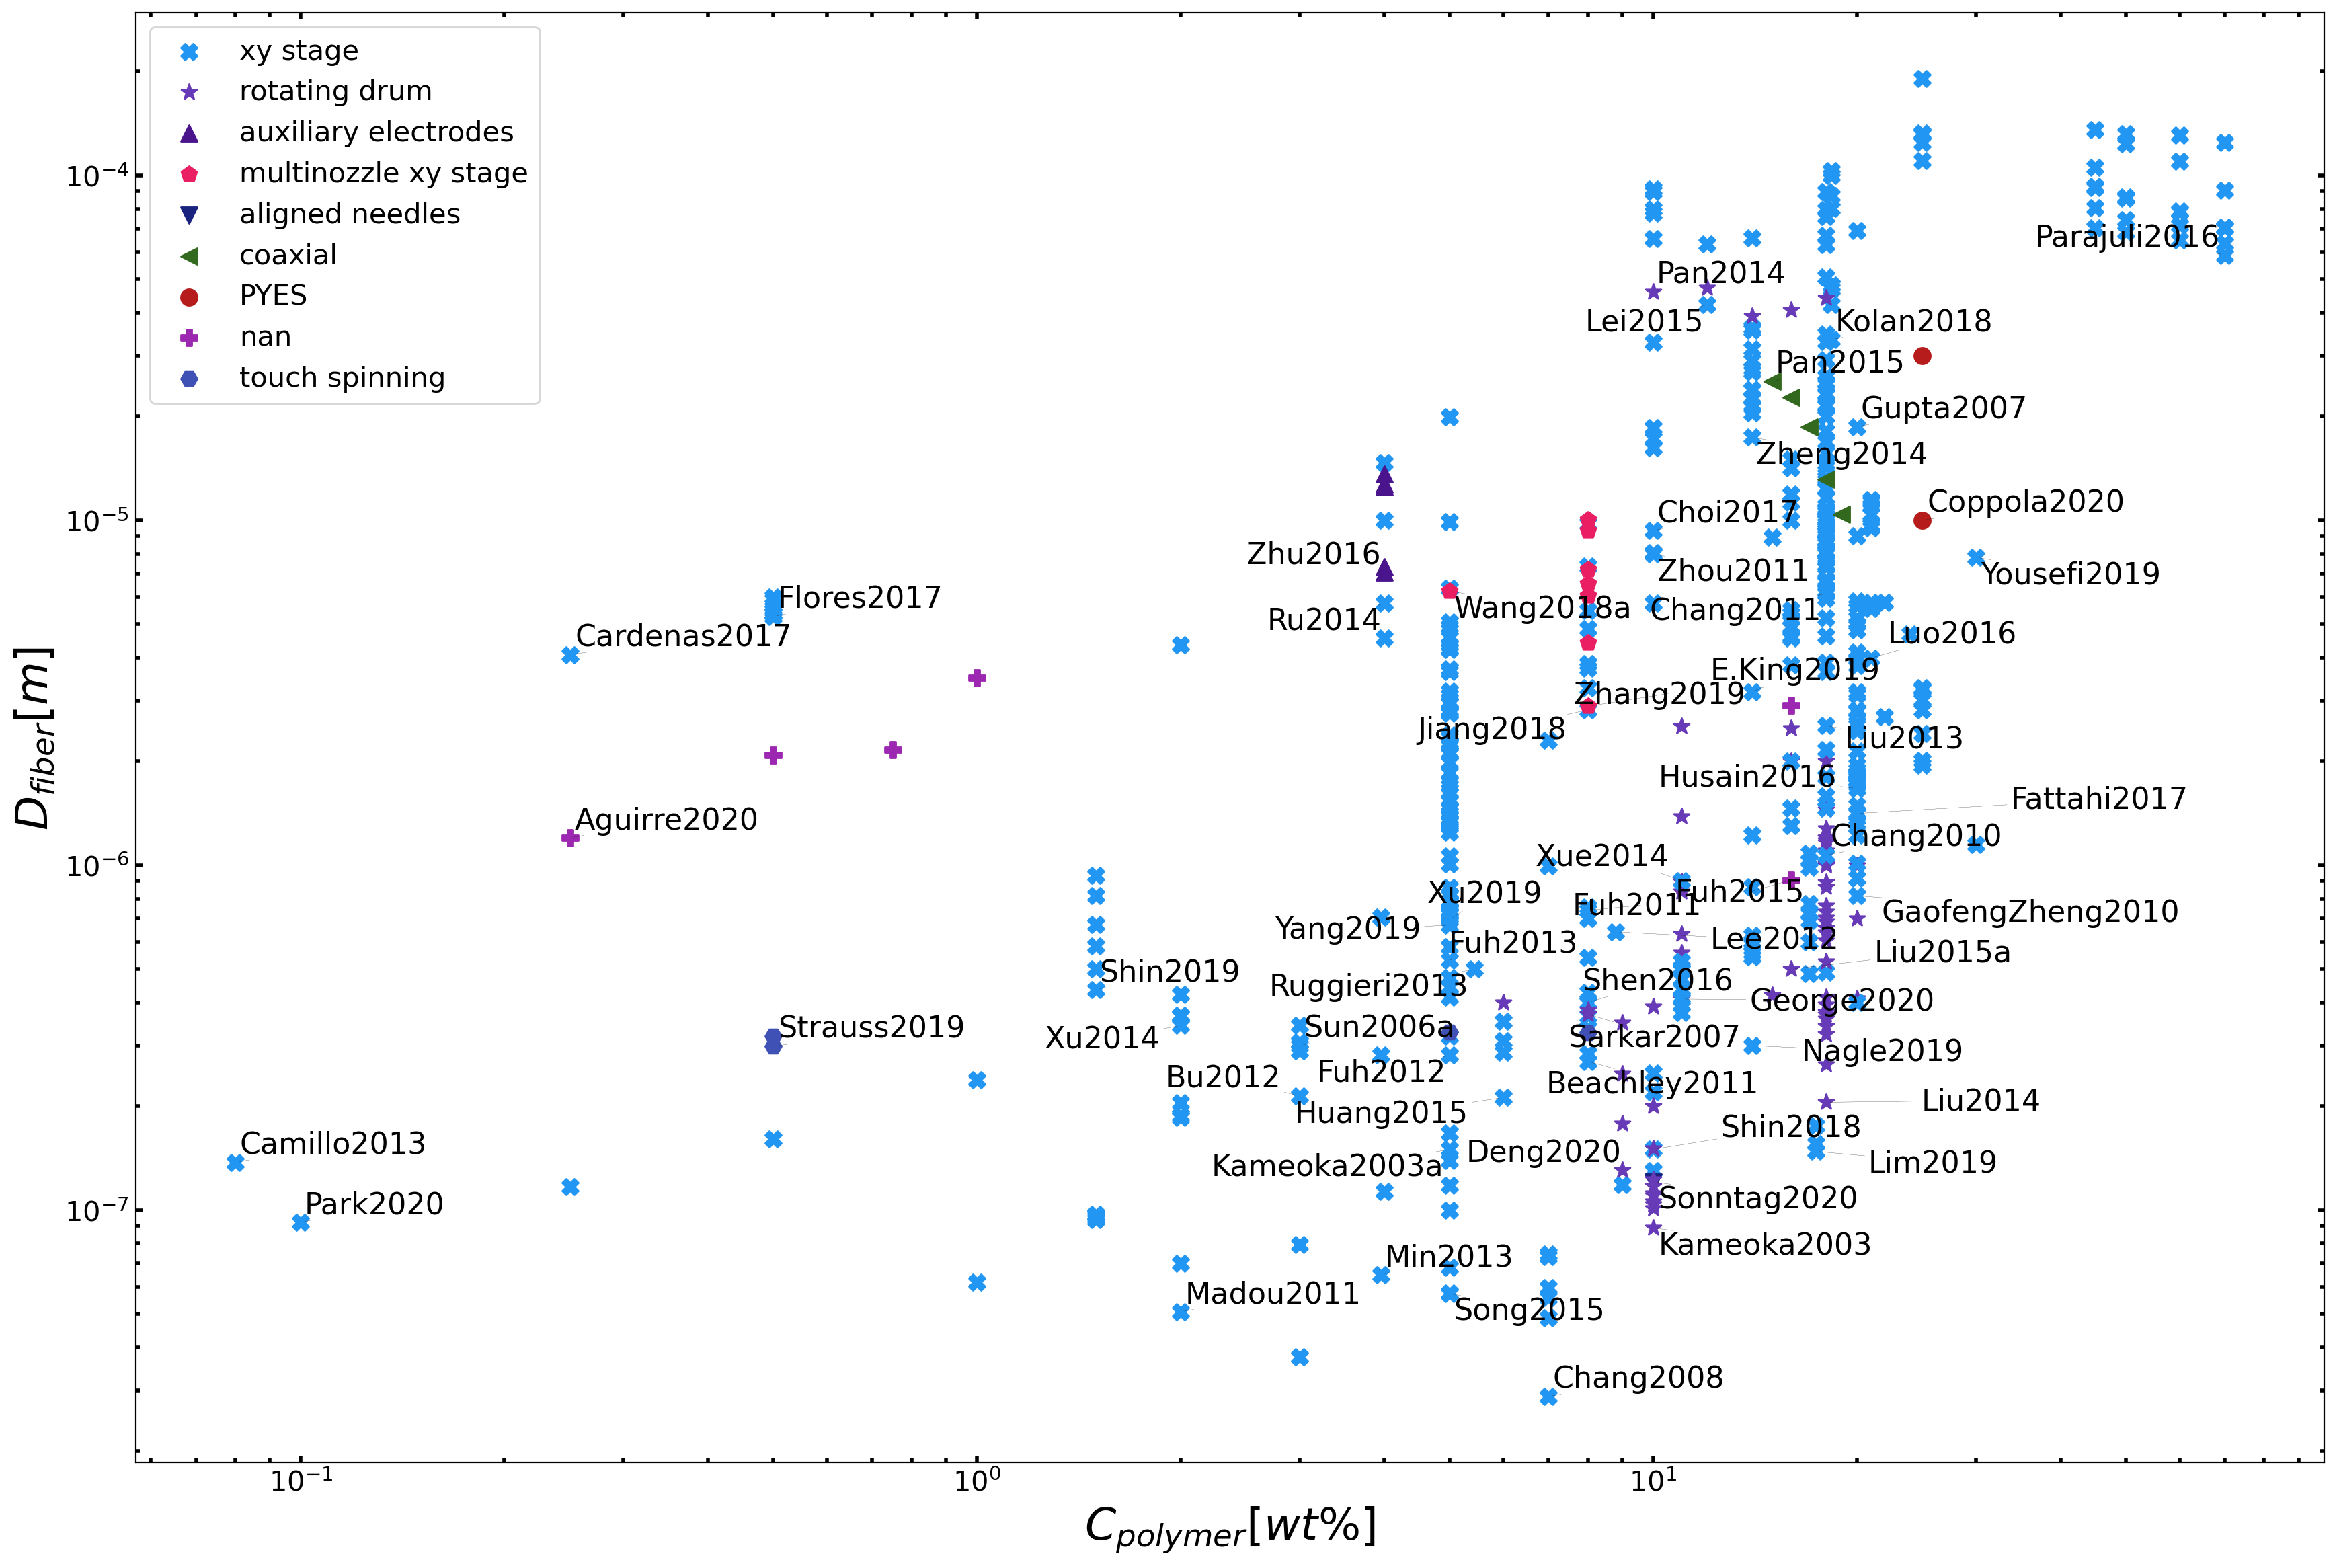
\includegraphics[width=\textwidth]{./Figures/plt_Cpolymerwt_vs_Dfiberm.png}
\decoRule
\caption[Scatter Plot of Polymer Concentrations and Fiber Diameters from Literature Experimental Results]{Scatter Plot of Polymer Concentrations and Fiber Diameters from Literature Experimental Results. \cite{
  Yang2019,Fattahi2017,Shin2019,Wang2015,Parajuli2016,Zheng2010,Fuh2011,Dalton2015,
  Ru2014,Xue2014,Wang2017,Xu2014,Liu2013,Pan2014,Canton2014,Chakraborty2009,Gupta2007,
  He2018,Zhou2011,Chen2013,Williams2018,Choi2017,Pan2019,Lei2015,Lim2019,Park2020,
  Fuh2012,Flores2017,Chang2010,Xu2019,Zhang2019,Shin2018,Fuh2015,Nagle2019,Zheng2012,
  Kameoka2003a,Liu2014,E.King2019,Hochleitner2017,Madou2011,Jiang2018,Husain2016,
  ElectrospinTech2015,Brown2011,Kolan2018,Chang2011,Beachley2011,Camillo2013,Kameoka2003,
  Bu2012,Lee2012,Huang2015,Coppola2020,CisquellaSerra2019,Ruggieri2013,Hochleitner2014,
  Zhu2016,Brown2014,Chang2008,Sonntag2020,Kim2018,Deng2020,Han2019,George2020,Sun2006a,
  Pan2015,Shen2016,Strauss2019,Fuh2013,Sarkar2007,You2017,Wang2018a,Zheng2014,Song2015,
  GaofengZheng2010,Liu2015a,Min2013,Luo2016,Yousefi2019,Cardenas2017,Coppola2014}}
\label{fig:plt_Cpolymerwt_vs_Dfiberm}
\end{figure}

The trend of Figure \ref{fig:plt_Dnozzlem_vs_Dfiberm} shows that thicker nozzle diameters yield thicker fibers. However, the final fiber diameter can be reduced without changing the nozzle diameter. For instance Chang et al. \cite{Chang2008} achieved the thinnest fibers of about $50 nm$ in diameter even though Chang implemented nozzle needles of similar diameter as Shin, Min and Xu by the implementation different settings on the other process parameters. \cite{Shin2019, Min2013, Xu2014} It is reasonable to notice that Chang's record of achieving the thinnest fiber may be a one time-successful since, neither the yield rate nor the reproducibility of their technique was not reported.

\begin{figure}[!th]
\centering
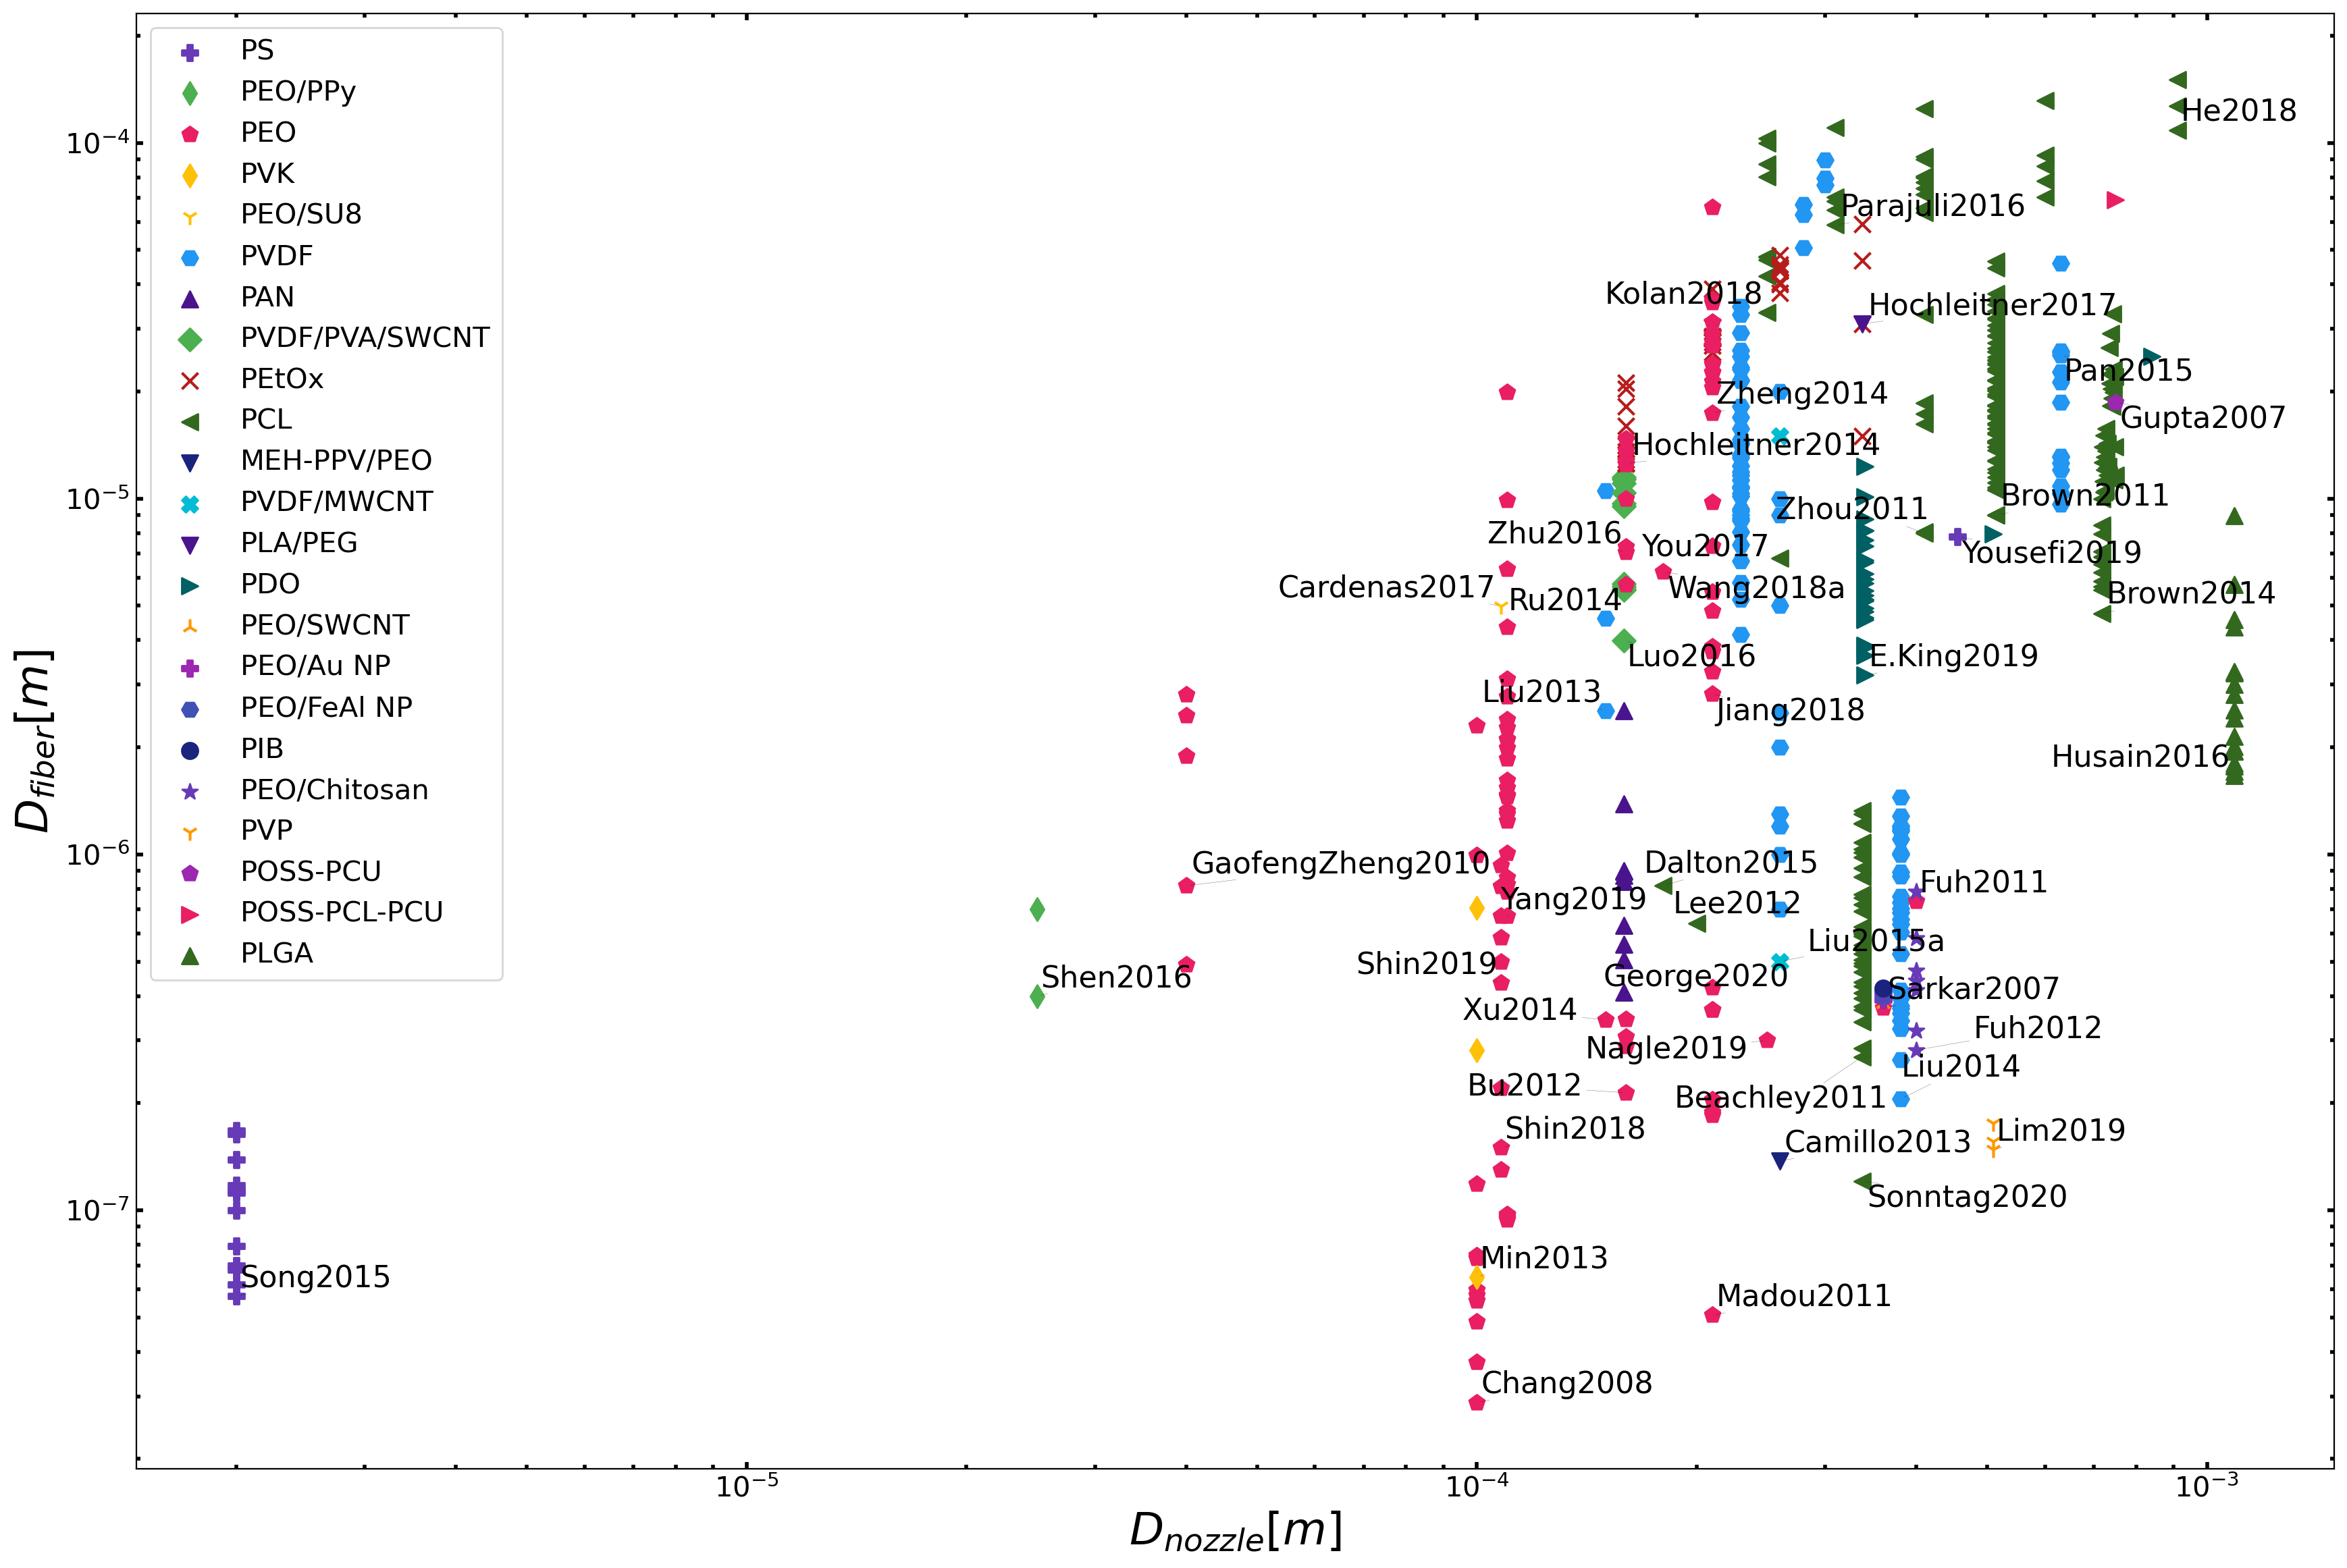
\includegraphics[width=\textwidth]{./Figures/plt_Dnozzlem_vs_Dfiberm.png}
\decoRule
\caption[Scatter Plot of Nozzle Inner Diameters and Fiber Diameters from Literature Experimental Results]{Scatter Plot of Nozzle Inner Diameters and Fiber Diameters from Literature Experimental Results. \cite{
  Yang2019,Fattahi2017,Shin2019,Wang2015,Parajuli2016,Zheng2010,Fuh2011,Dalton2015,
  Ru2014,Xue2014,Wang2017,Xu2014,Liu2013,Pan2014,Canton2014,Chakraborty2009,Gupta2007,
  He2018,Zhou2011,Chen2013,Williams2018,Choi2017,Pan2019,Lei2015,Lim2019,Park2020,
  Fuh2012,Flores2017,Chang2010,Xu2019,Zhang2019,Shin2018,Fuh2015,Nagle2019,Zheng2012,
  Kameoka2003a,Liu2014,E.King2019,Hochleitner2017,Madou2011,Jiang2018,Husain2016,
  ElectrospinTech2015,Brown2011,Kolan2018,Chang2011,Beachley2011,Camillo2013,Kameoka2003,
  Bu2012,Lee2012,Huang2015,Coppola2020,CisquellaSerra2019,Ruggieri2013,Hochleitner2014,
  Zhu2016,Brown2014,Chang2008,Sonntag2020,Kim2018,Deng2020,Han2019,George2020,Sun2006a,
  Pan2015,Shen2016,Strauss2019,Fuh2013,Sarkar2007,You2017,Wang2018a,Zheng2014,Song2015,
  GaofengZheng2010,Liu2015a,Min2013,Luo2016,Yousefi2019,Cardenas2017,Coppola2014}}
\label{fig:plt_Dnozzlem_vs_Dfiberm}
\end{figure}

The relationship between the fiber diameter the working distance $L$ and applied voltage $\Phi_0$ can be depicted in Figures \ref{fig:plt_Lm_vs_Dfiberm} and \ref{fig:plt_Phi0V_vs_Dfiberm}. The near-field electrospinning jet is ejected from the Taylor cone when the applied voltage generates an electric field strong enough to break the solution drop. Changing the applied voltage will amend initial drop and fiber morphology, thereby resulting in a change in the fibers' properties. However, the effect of the applied voltage on the fiber diameter is not well defined. On one hand, many researchers posit that high applied voltages lead to larger fiber diameters, whereas other researchers have reported reductions in fiber diameter with high applied voltages as the electric field force increases on the charged jet. \cite{Zhang2005} Furthermore, Reneker and Chun observed that applied voltage does not significantly affect the diameter of electrospun polyethylene oxide (PEO) fibers. \cite{Reneker1996} Applied voltage has an influence on the fiber diameter, but the degree and direction of influence varies with other process parameters such as polymeric solution concentration and on the working distance \cite{Yordem2008, Chang2016}.

Looking at Figures \ref{fig:plt_Lm_vs_Dfiberm} and \ref{fig:plt_Phi0V_vs_Dfiberm}, the data points from Husain, Lee and Sonntag \cite{Husain2016, Lee2012, Sonntag2020} experimental results are outside the principal cluster since they implemented working distances around $10^{-1} \textrm{m}$, which is concidered to be the threshold between NFES and far-field electrospinning (FFES). One can observe that: a) in NFES fiber diameter increase with increasing applied voltage; and b) in FFES fiber diameter decrease with increasing applied voltage. On the other hand, data related to Liu's and Beachey's work \cite{Liu2014, Beachey2011} do not fit the main trend as they perform the electrospinning process with a rotating drum as the collector, instead of the typical xy stage.

\begin{figure}[!th]
\centering
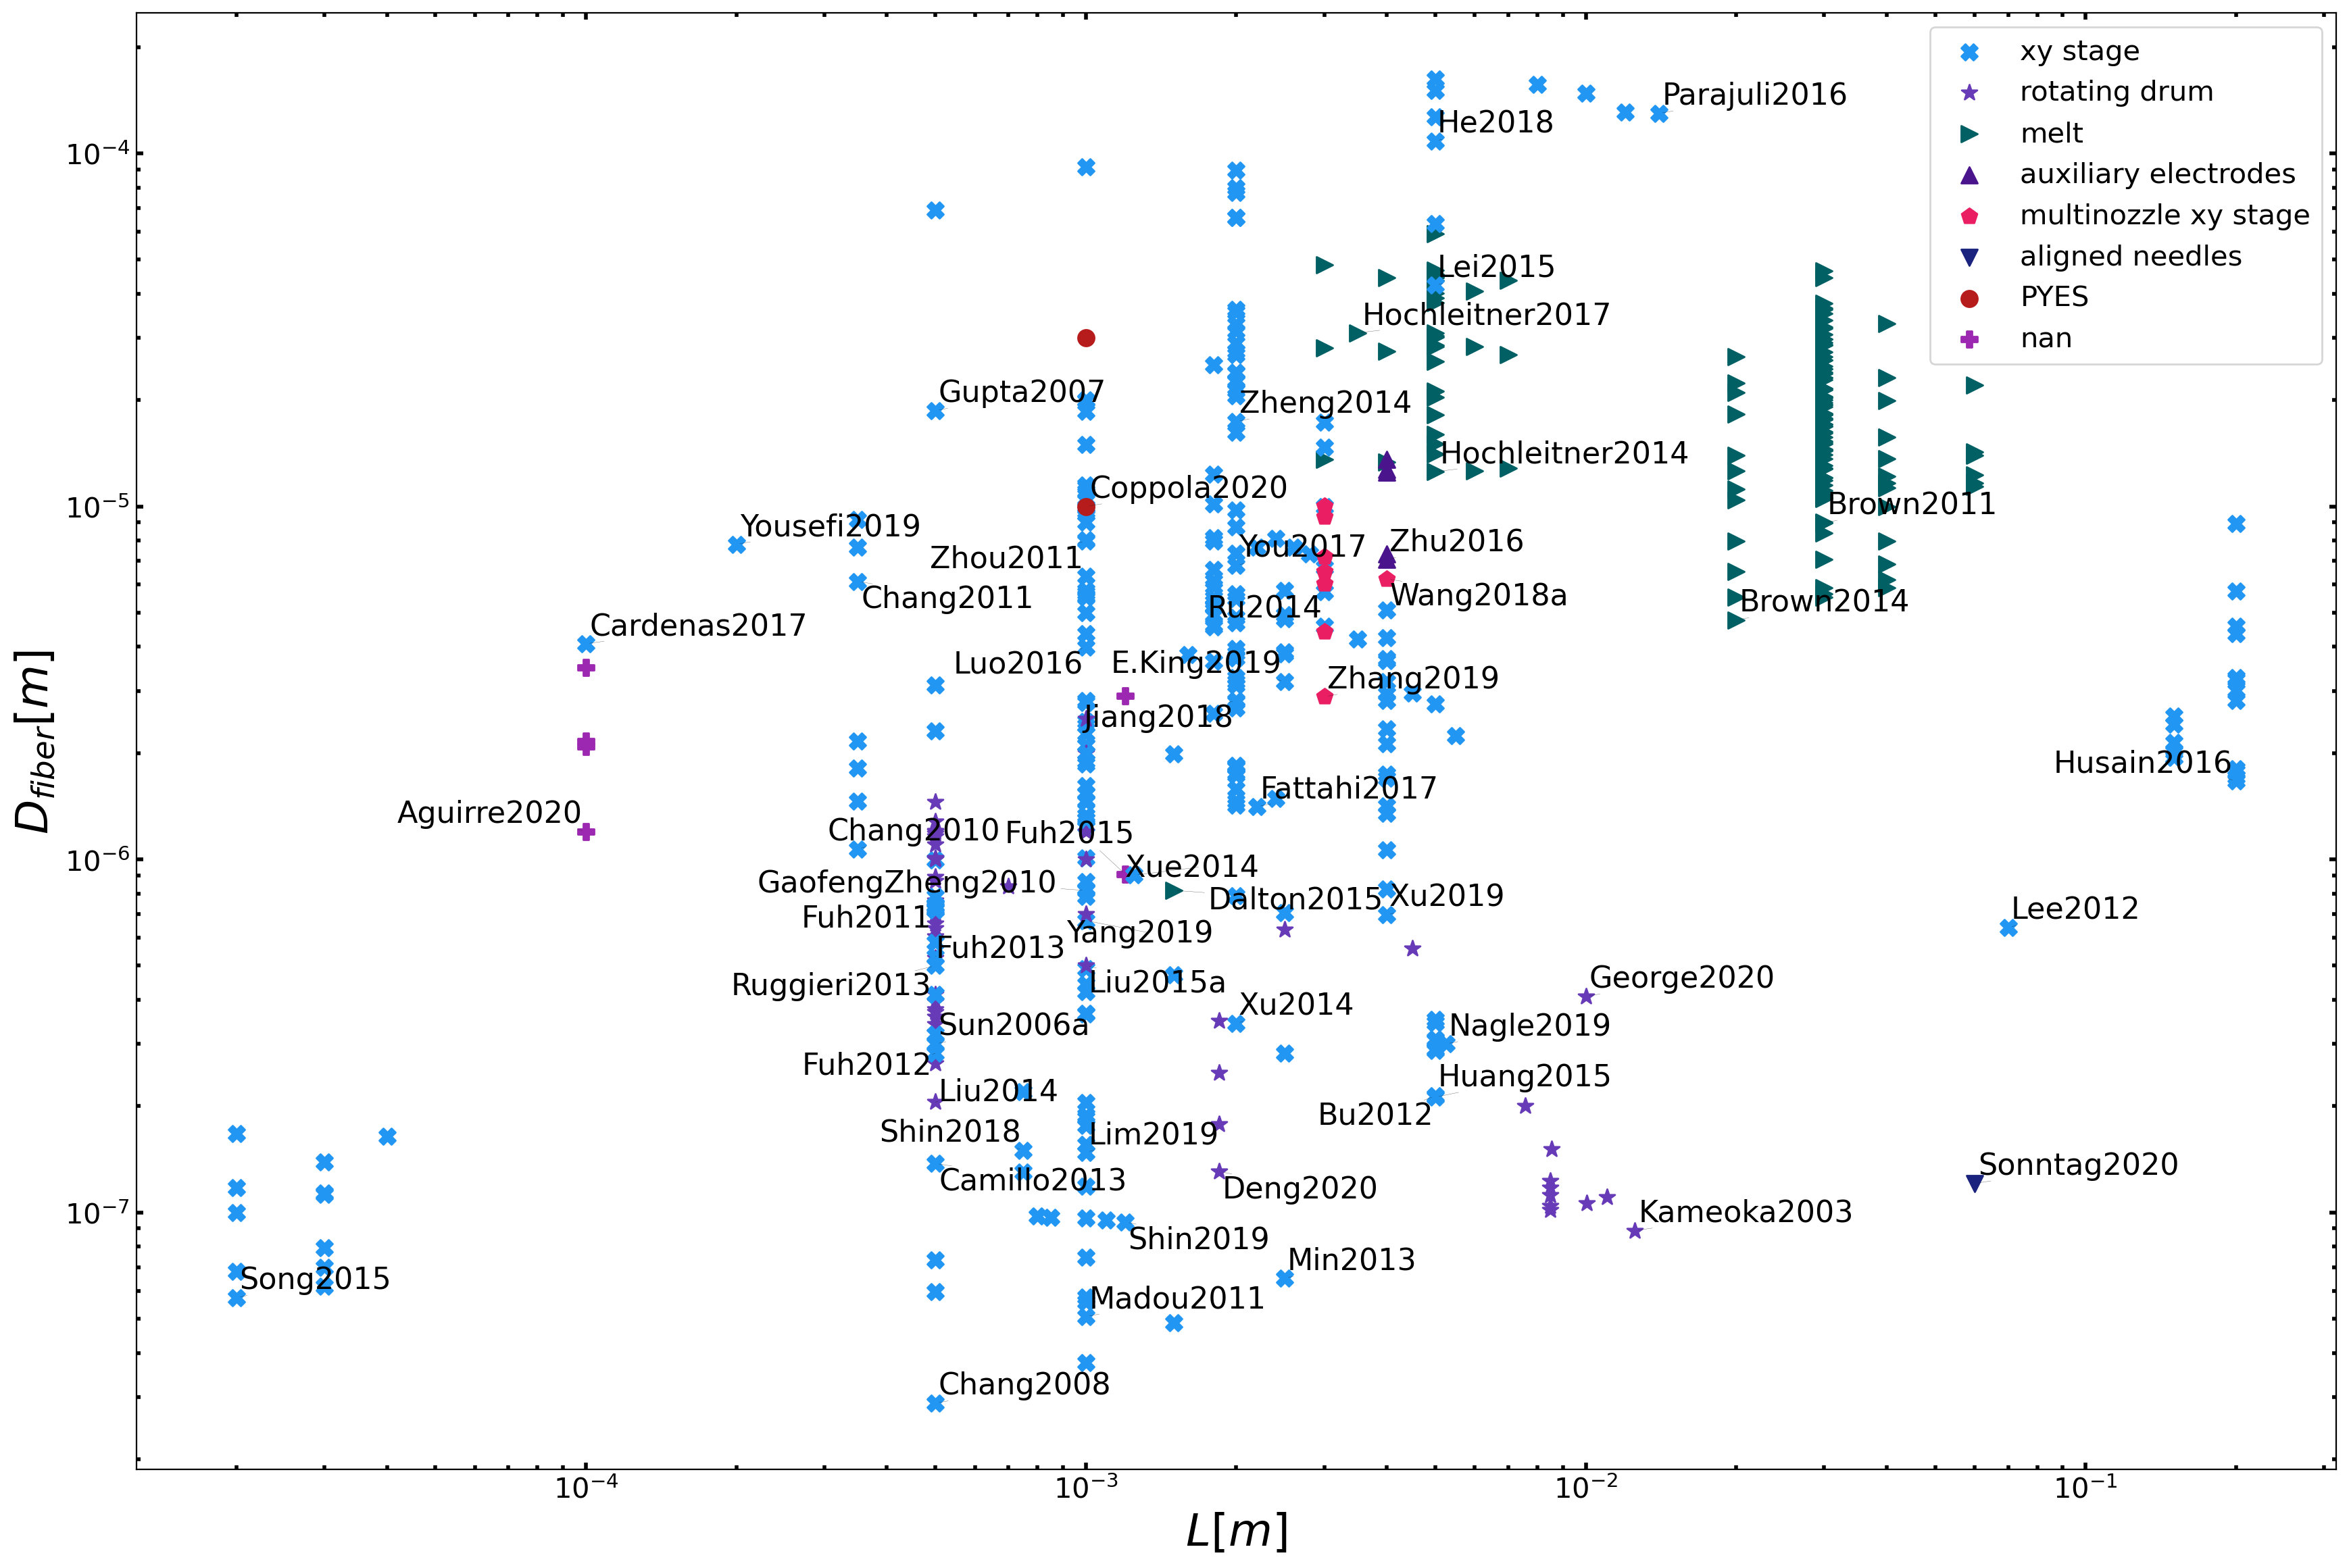
\includegraphics[width=\textwidth]{./Figures/plt_Lm_vs_Dfiberm.png}
\decoRule
\caption[Scatter Plot of NFES Working Distances and Fiber Diameters from Literature Experimental Results]{Scatter Plot of NFES Working Distances and Fiber Diameters from Literature Experimental Results. \cite{
  Yang2019,Fattahi2017,Shin2019,Wang2015,Parajuli2016,Zheng2010,Fuh2011,Dalton2015,
  Ru2014,Xue2014,Wang2017,Xu2014,Liu2013,Pan2014,Canton2014,Chakraborty2009,Gupta2007,
  He2018,Zhou2011,Chen2013,Williams2018,Choi2017,Pan2019,Lei2015,Lim2019,Park2020,
  Fuh2012,Flores2017,Chang2010,Xu2019,Zhang2019,Shin2018,Fuh2015,Nagle2019,Zheng2012,
  Kameoka2003a,Liu2014,E.King2019,Hochleitner2017,Madou2011,Jiang2018,Husain2016,
  ElectrospinTech2015,Brown2011,Kolan2018,Chang2011,Beachley2011,Camillo2013,Kameoka2003,
  Bu2012,Lee2012,Huang2015,Coppola2020,CisquellaSerra2019,Ruggieri2013,Hochleitner2014,
  Zhu2016,Brown2014,Chang2008,Sonntag2020,Kim2018,Deng2020,Han2019,George2020,Sun2006a,
  Pan2015,Shen2016,Strauss2019,Fuh2013,Sarkar2007,You2017,Wang2018a,Zheng2014,Song2015,
  GaofengZheng2010,Liu2015a,Min2013,Luo2016,Yousefi2019,Cardenas2017,Coppola2014}}
\label{fig:plt_Lm_vs_Dfiberm}
\end{figure}

\begin{figure}[!th]
\centering
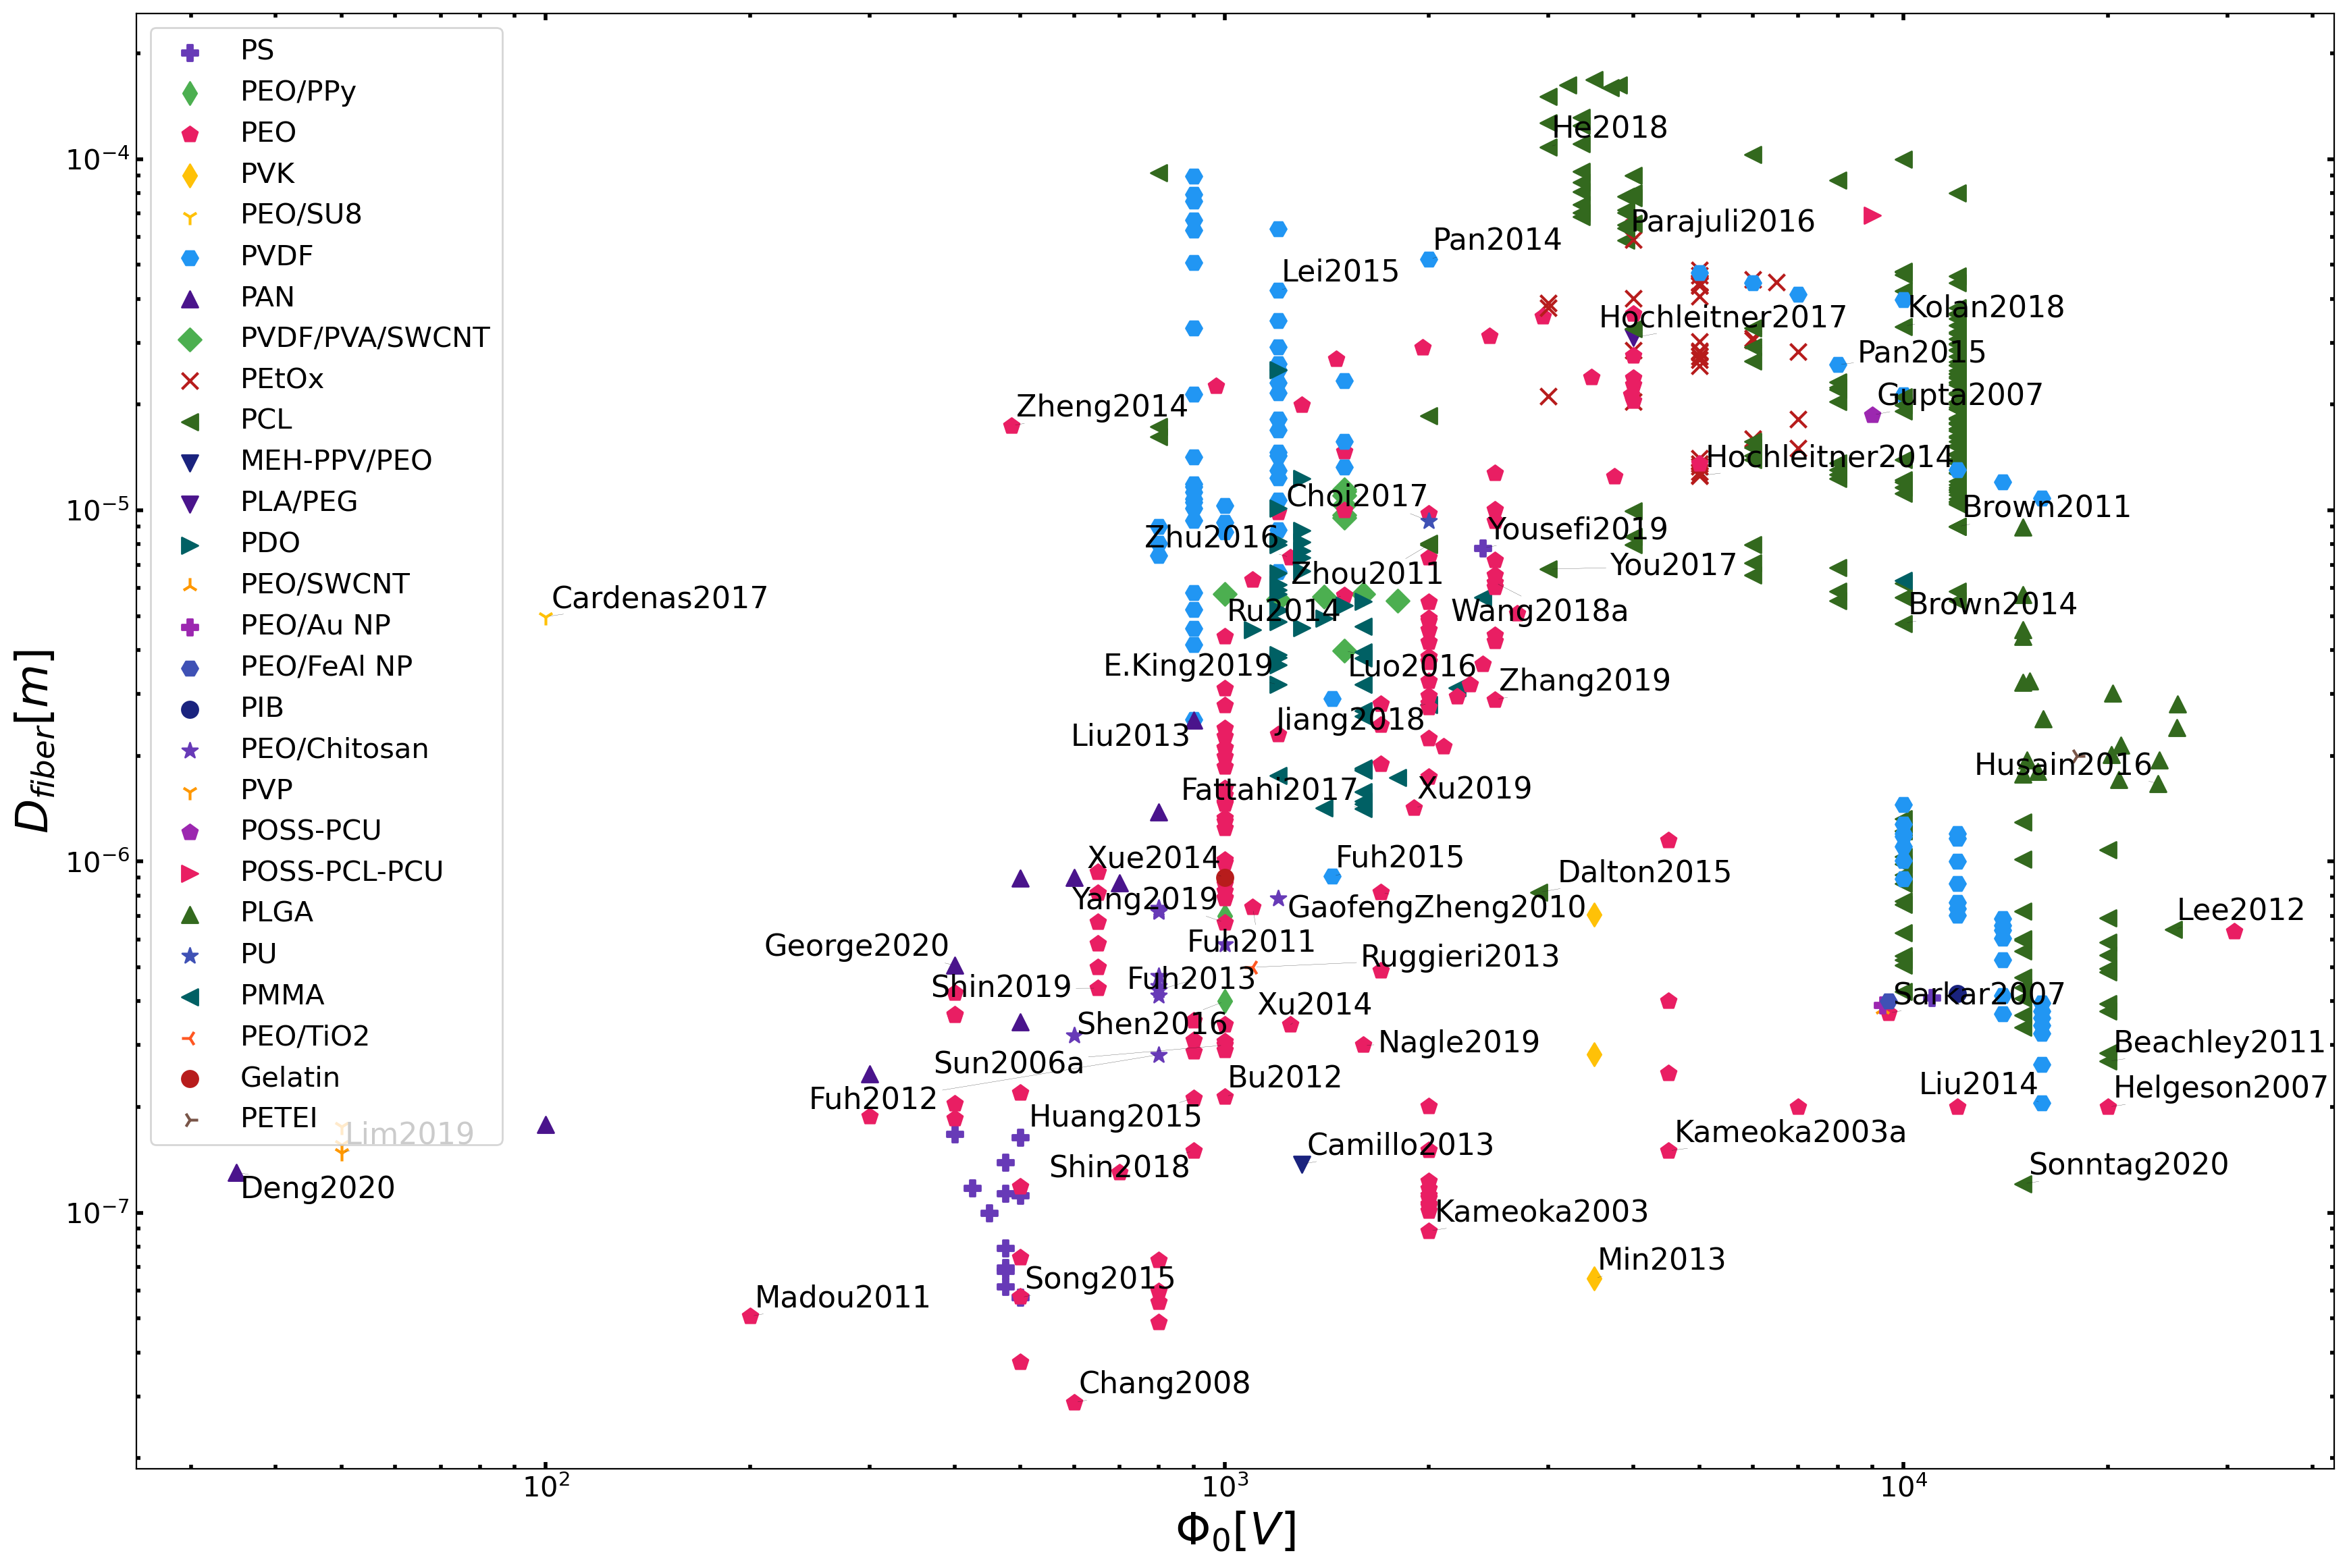
\includegraphics[width=\textwidth]{./Figures/plt_Phi0V_vs_Dfiberm.png}
\decoRule
\caption[Scatter Plot of NFES Applied Voltages and Fiber Diameters from Literature Experimental Results]{Scatter Plot of NFES Applied Voltages and Fiber Diameters from Literature Experimental Results. \cite{
  Yang2019,Fattahi2017,Shin2019,Wang2015,Parajuli2016,Zheng2010,Fuh2011,Dalton2015,
  Ru2014,Xue2014,Wang2017,Xu2014,Liu2013,Pan2014,Canton2014,Chakraborty2009,Gupta2007,
  He2018,Zhou2011,Chen2013,Williams2018,Choi2017,Pan2019,Lei2015,Lim2019,Park2020,
  Fuh2012,Flores2017,Chang2010,Xu2019,Zhang2019,Shin2018,Fuh2015,Nagle2019,Zheng2012,
  Kameoka2003a,Liu2014,E.King2019,Hochleitner2017,Madou2011,Jiang2018,Husain2016,
  ElectrospinTech2015,Brown2011,Kolan2018,Chang2011,Beachley2011,Camillo2013,Kameoka2003,
  Bu2012,Lee2012,Huang2015,Coppola2020,CisquellaSerra2019,Ruggieri2013,Hochleitner2014,
  Zhu2016,Brown2014,Chang2008,Sonntag2020,Kim2018,Deng2020,Han2019,George2020,Sun2006a,
  Pan2015,Shen2016,Strauss2019,Fuh2013,Sarkar2007,You2017,Wang2018a,Zheng2014,Song2015,
  GaofengZheng2010,Liu2015a,Min2013,Luo2016,Yousefi2019,Cardenas2017,Coppola2014}}
\label{fig:plt_Phi0V_vs_Dfiberm}
\end{figure}



\begin{figure}[!th]
\centering
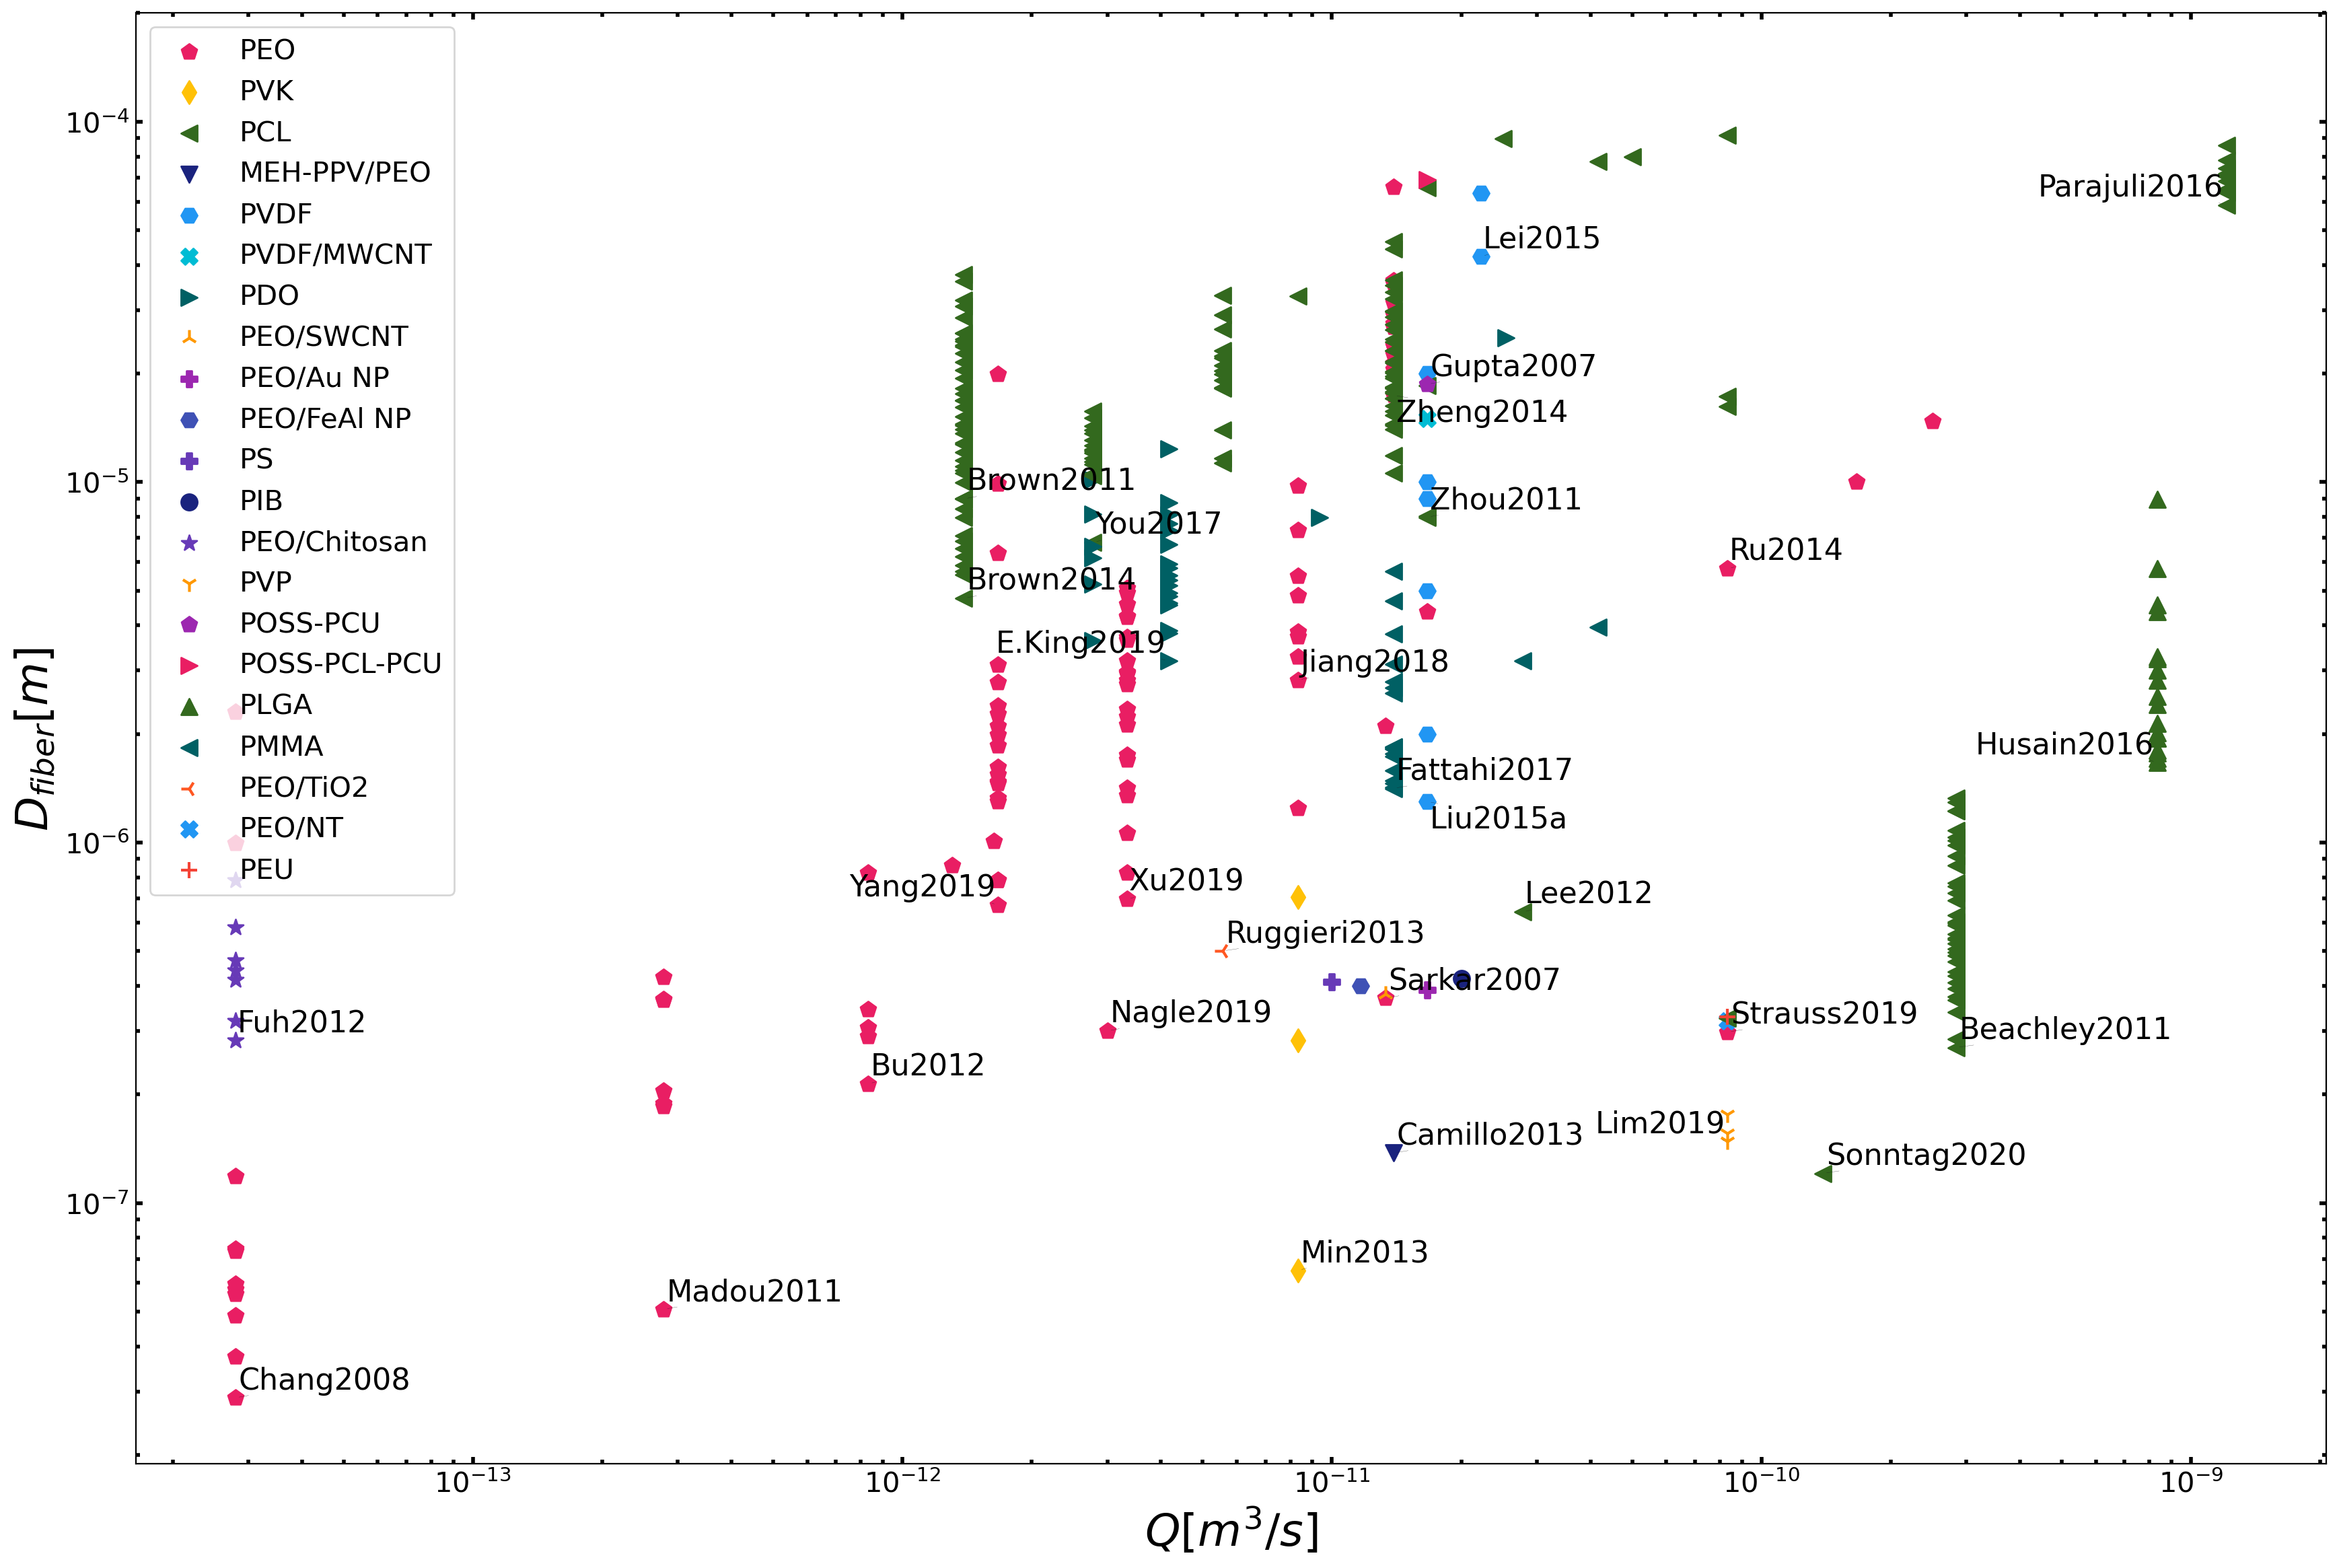
\includegraphics[width=\textwidth]{./Figures/plt_Qm3s_vs_Dfiberm.png}
\decoRule
\caption[Scatter Plot of Polymer Solution Flow Rates and Fiber Diameters from Literature Experimental Results]{Scatter Plot of Polymer Solution Flow Rates and Fiber Diameters from Literature Experimental Results. \cite{
  Yang2019,Fattahi2017,Shin2019,Wang2015,Parajuli2016,Zheng2010,Fuh2011,Dalton2015,
  Ru2014,Xue2014,Wang2017,Xu2014,Liu2013,Pan2014,Canton2014,Chakraborty2009,Gupta2007,
  He2018,Zhou2011,Chen2013,Williams2018,Choi2017,Pan2019,Lei2015,Lim2019,Park2020,
  Fuh2012,Flores2017,Chang2010,Xu2019,Zhang2019,Shin2018,Fuh2015,Nagle2019,Zheng2012,
  Kameoka2003a,Liu2014,E.King2019,Hochleitner2017,Madou2011,Jiang2018,Husain2016,
  ElectrospinTech2015,Brown2011,Kolan2018,Chang2011,Beachley2011,Camillo2013,Kameoka2003,
  Bu2012,Lee2012,Huang2015,Coppola2020,CisquellaSerra2019,Ruggieri2013,Hochleitner2014,
  Zhu2016,Brown2014,Chang2008,Sonntag2020,Kim2018,Deng2020,Han2019,George2020,Sun2006a,
  Pan2015,Shen2016,Strauss2019,Fuh2013,Sarkar2007,You2017,Wang2018a,Zheng2014,Song2015,
  GaofengZheng2010,Liu2015a,Min2013,Luo2016,Yousefi2019,Cardenas2017,Coppola2014}}
\label{fig:plt_Qm3s_vs_Dfiberm}
\end{figure}

\begin{figure}[!th]
\centering
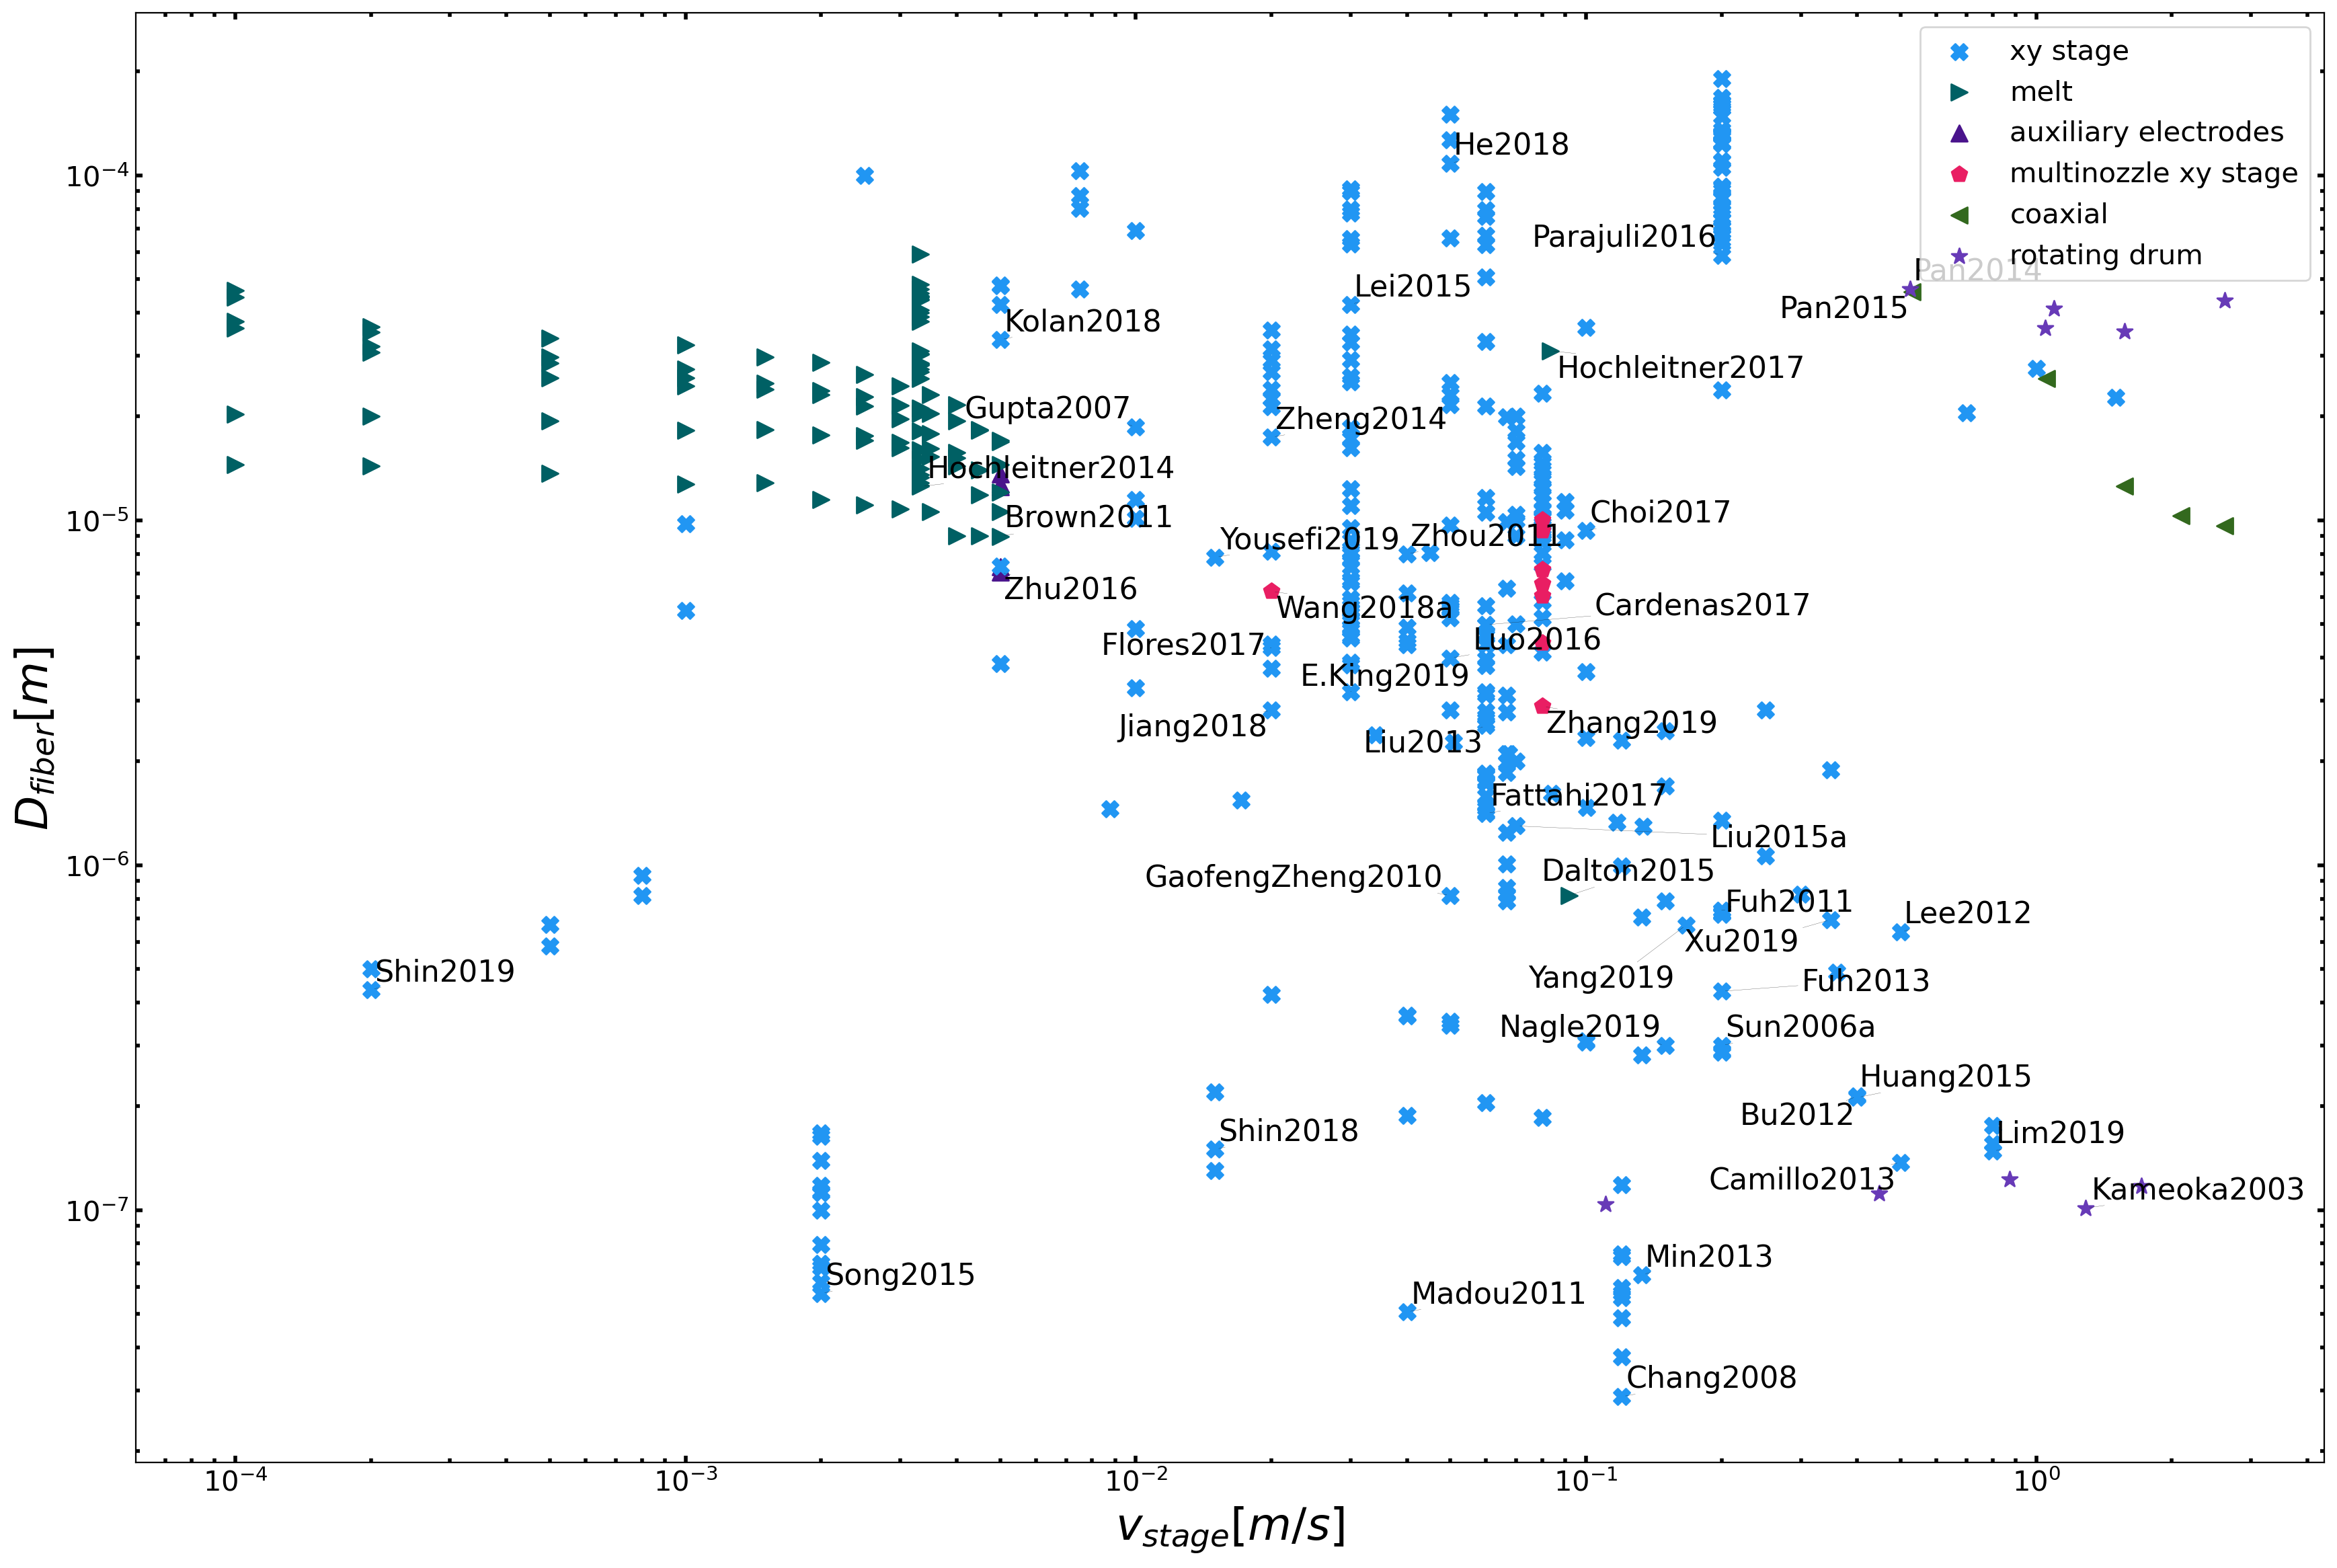
\includegraphics[width=\textwidth]{./Figures/plt_vstagems_vs_Dfiberm.png}
\decoRule
\caption[Scatter Plot of Collector xy Stage Velocities and Fiber Diameters from Literature Experimental Results]{Scatter Plot of Collector xy Stage Velocities and Fiber Diameters from Literature Experimental Results. \cite{
  Yang2019,Fattahi2017,Shin2019,Wang2015,Parajuli2016,Zheng2010,Fuh2011,Dalton2015,
  Ru2014,Xue2014,Wang2017,Xu2014,Liu2013,Pan2014,Canton2014,Chakraborty2009,Gupta2007,
  He2018,Zhou2011,Chen2013,Williams2018,Choi2017,Pan2019,Lei2015,Lim2019,Park2020,
  Fuh2012,Flores2017,Chang2010,Xu2019,Zhang2019,Shin2018,Fuh2015,Nagle2019,Zheng2012,
  Kameoka2003a,Liu2014,E.King2019,Hochleitner2017,Madou2011,Jiang2018,Husain2016,
  ElectrospinTech2015,Brown2011,Kolan2018,Chang2011,Beachley2011,Camillo2013,Kameoka2003,
  Bu2012,Lee2012,Huang2015,Coppola2020,CisquellaSerra2019,Ruggieri2013,Hochleitner2014,
  Zhu2016,Brown2014,Chang2008,Sonntag2020,Kim2018,Deng2020,Han2019,George2020,Sun2006a,
  Pan2015,Shen2016,Strauss2019,Fuh2013,Sarkar2007,You2017,Wang2018a,Zheng2014,Song2015,
  GaofengZheng2010,Liu2015a,Min2013,Luo2016,Yousefi2019,Cardenas2017,Coppola2014}}
\label{fig:plt_vstagems_vs_Dfiberm}
\end{figure}


The effect of parameters such as ink concentration, working distance, applied voltage, and stage speed on the diameter of the printed nano-fibers was investigated, a summary is presented in Table \ref{tab:nfesProcessParameters}.

\begin{table}[ht]
\centering
\caption[Near-Field Electrospinning Process Parameters]{Summary of the main parameters that drive the electrospinning process, ordered by: polymer solution parameters, process parameters, and ambient parameters. Adapted from \cite{Bagbi2019, Unnithan2015}}
\begin{tabularx}{\textwidth}{lX}
\hline
\textbf{NFES Process Parameters} & \textbf{Effect} \\
\hline
\textbf{Solution Parameters:} &  \\
Concentration & Concentration shall be high enough to produce uniform nano-fibers, but low enough to give the correct viscosity \\
Molecular weight & High molecular weight polymers yield smoother fibers \\
Viscosity & Zero-shear viscosity shall be optimal to generate a constant jet from the needle \\
Conductivity & Solution shall be conductive enough for the electrif field to have influence on the jet \\
\textbf{Process Parameters:} &  \\
Applied voltage & Higher voltages eject more material from the nozzle \\
Flow rate & Slow flow rates yield thinner fibers, but it shall be fast enough to prevent clogging and keep the Tailor cone in a constant size and shape \\
Working distance & Long distances result in thinner fibers, however the spatial control is harmed \\
\textbf{Ambient Parameters:} &  \\
Humidity & Increasing humidity produces thicker diameters \\
Temperature & Increasing temperature yields thinner fibers, however high temperatures make the nozzle prone to clog as the solvent evaporates at a faster rate \\
\hline
\end{tabularx}
\label{tab:nfesProcessParameters}
\end{table}

Near-field electrospinning (NFES) is known as a versatile nano-fabrication technique, suitable for several applications such as tissue engineering, chemical sensing, filtration, energy storage, besides others (see Figure \ref{fig:synthesesAndApplicationsOfNanofibers}). Fast developments in electrospinning has been observed in recent years. However, this process is limited by the electric field wiping instability effects during polymer deposition. This leads to a major challenge: how to surpass this limitation of planar two-dimensional prints. The current trend in this area lies on the research of new materials, techniques to increase precision patterning in NFES systems.

\begin{figure}[!th]
\centering
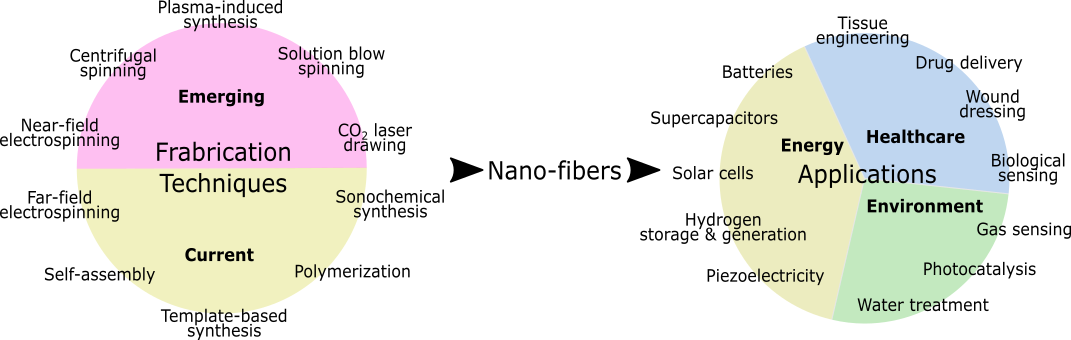
\includegraphics[width=\textwidth]{./Figures/synthesesAndApplicationsOfNanofibers.png}
\decoRule
\caption[Syntheses and Applications of Nanofibers]{Syntheses and Applications of Nanofibers. Adapted from \cite{Kenry2017}}
\label{fig:synthesesAndApplicationsOfNanofibers}
\end{figure}

\section{Diameter Prediction of Electrospun Fibers} % adimensional analysis



\begin{figure}[!th]
\centering
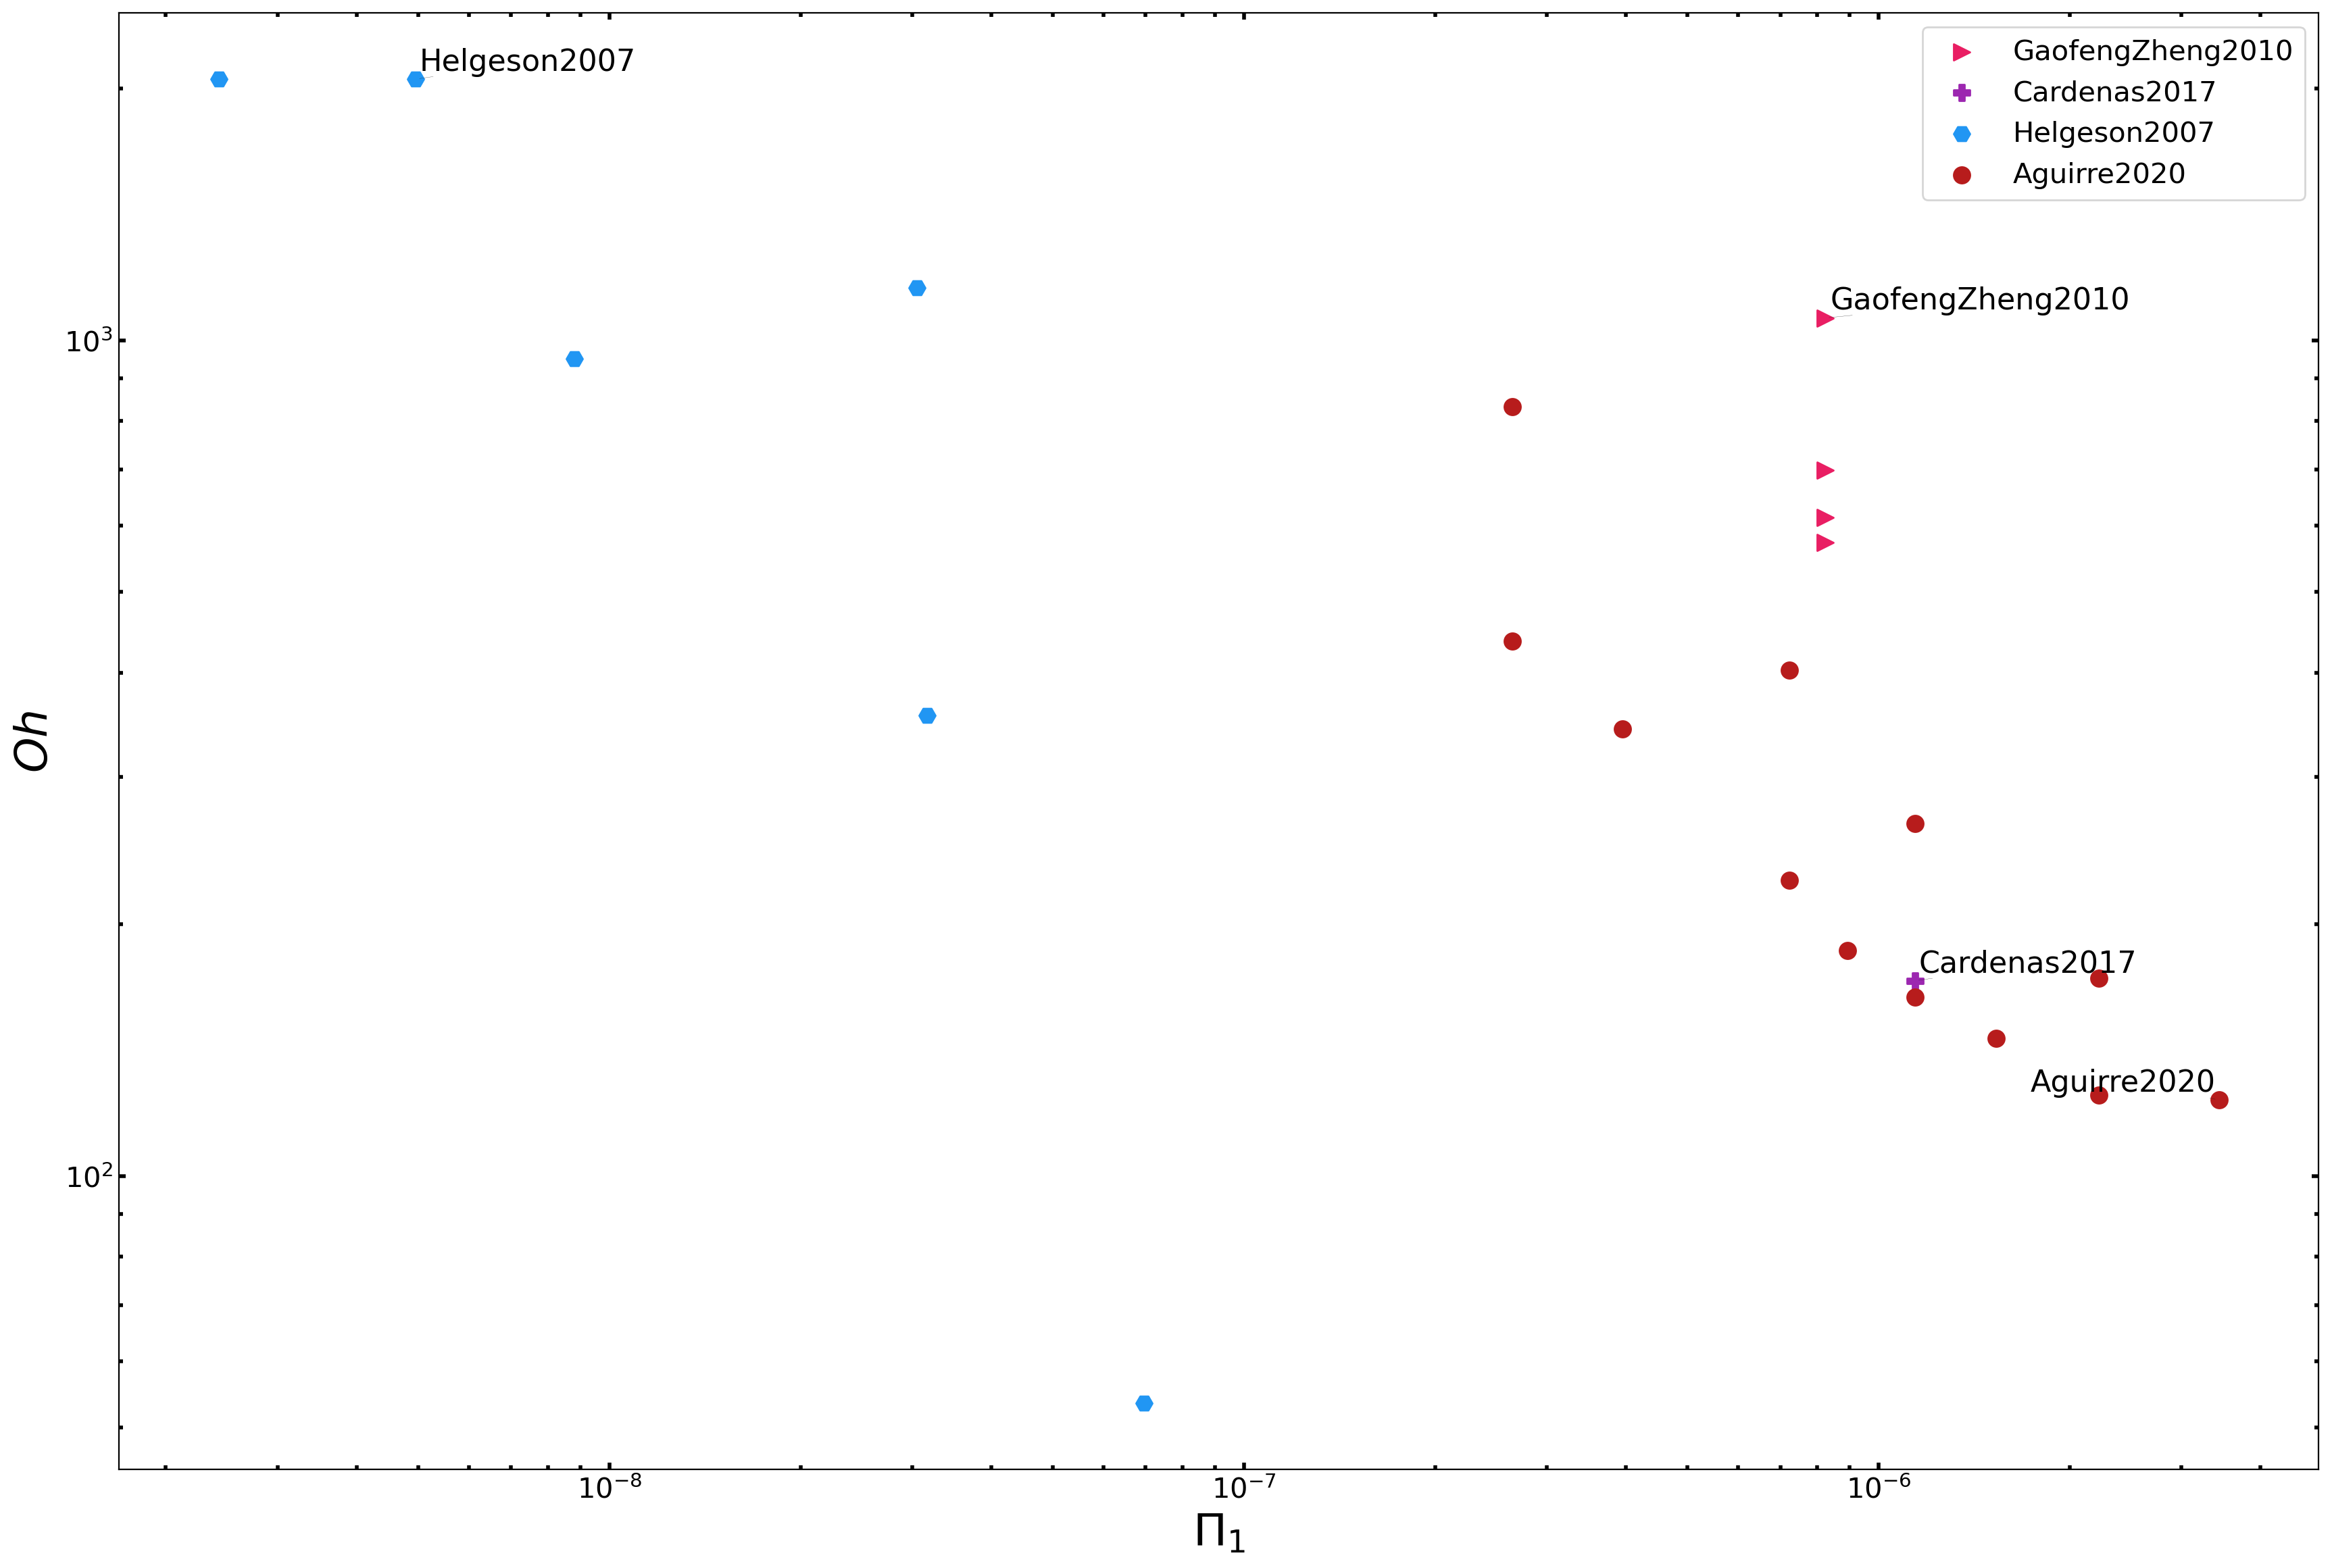
\includegraphics[width=\textwidth]{./Figures/plt_Pi1_vs_Oh.png}
\decoRule
\caption[Image Analysis Algorithm to Measure Fiber Diameters from SEM images]{Image Analysis Algorithm to Measure Fiber Diameters from SEM images. Ilustration uses Yousefi et al.'s work as an example. \cite{Helgeson2007,
  Yang2019,Fattahi2017,Shin2019,Wang2015,Parajuli2016,Zheng2010,Fuh2011,Dalton2015,
  Ru2014,Xue2014,Wang2017,Xu2014,Liu2013,Pan2014,Canton2014,Chakraborty2009,Gupta2007,
  He2018,Zhou2011,Chen2013,Williams2018,Choi2017,Pan2019,Lei2015,Lim2019,Park2020,
  Fuh2012,Flores2017,Chang2010,Xu2019,Zhang2019,Shin2018,Fuh2015,Nagle2019,Zheng2012,
  Kameoka2003a,Liu2014,E.King2019,Hochleitner2017,Madou2011,Jiang2018,Husain2016,
  ElectrospinTech2015,Brown2011,Kolan2018,Chang2011,Beachley2011,Camillo2013,Kameoka2003,
  Bu2012,Lee2012,Huang2015,Coppola2020,CisquellaSerra2019,Ruggieri2013,Hochleitner2014,
  Zhu2016,Brown2014,Chang2008,Sonntag2020,Kim2018,Deng2020,Han2019,George2020,Sun2006a,
  Pan2015,Shen2016,Strauss2019,Fuh2013,Sarkar2007,You2017,Wang2018a,Zheng2014,Song2015,
  GaofengZheng2010,Liu2015a,Min2013,Luo2016,Yousefi2019,Cardenas2017,Coppola2014}}
\label{fig:plt_Pi1_vs_Oh}
\end{figure}
% Chapter Template

\chapter{Selection of Compatible Polymer-Solvent Combinations for Near-Field Electrospinning and Pyrolysis} % Main chapter title

\label{Chapter:3}

% search : electrospunable capacity vs. thermo analysis of polymers in solutions (bad/good solvents)

%----------------------------------------------------------------------------------------
%	SECTION 1
%----------------------------------------------------------------------------------------
\section{Selection of Candidate Spunable Polymer Solutions}

%high molecular weight, polymer-solution interaction (straight chains)


\subsection{Rheology of candidate polymer solutions}



%----------------------------------------------------------------------------------------
%	SECTION 1
%----------------------------------------------------------------------------------------
\section{Effect of aromatic groups in oxygen-free polymers in NFES and Pyrolysis}



\section{\emph{conclude with a collection of potential spunable polymer solutions}}
% Chapter Template

\chapter{Fabrication and Characterization of Polymeric Fibers through Near-Field Electrospinning, and Forward-thinking on Photopolymerization and Pyrolysis} % Main chapter title

\label{Chapter:4}

%----------------------------------------------------------------------------------------
%	SECTION 1
%----------------------------------------------------------------------------------------
\section{}



%----------------------------------------------------------------------------------------
%	SECTION 2
%----------------------------------------------------------------------------------------
\section{}



%----------------------------------------------------------------------------------------
%	SECTION 3
%----------------------------------------------------------------------------------------
\section{Fabrication and Characterization of Legacy SU-8 carbon fibers}



%----------------------------------------------------------------------------------------
%	SECTION 3
%----------------------------------------------------------------------------------------
\section{Comparison of the Obtained Polymer Fibres Against SU8-based Carbon Fibres and Potential Applications}
% Were the selected candidates electrospunable?
% Fiber morphology



\section{\emph{conclude with fibre morphology before and after pyrolysis. determine best pyrolysis process}}
%Were the selected candidates electrospunable?
%Fiber morphology
%Yield rate
%Carbon content
%Conductivity
%Fiber morphology
% Chapter Template

\chapter{Concluding Remarks} % Main chapter title

\label{Chapter:5}

%----------------------------------------------------------------------------------------
%	SECTION 1
%----------------------------------------------------------------------------------------
\section{}



\section{Future work}
%Were the selected candidates electrospunable?
%Fiber morphology

% Chapter Template

\chapter{} % Main chapter title

\label{Chapter:6}

%----------------------------------------------------------------------------------------
%	SECTION 1
%----------------------------------------------------------------------------------------
\section{}



%% Chapter Template

\chapter{Comparison of the Carbon Fibers Obtained Against SU8-based Carbon Fibers and Potential Applications} % Main chapter title

\label{Chapter:7}

%----------------------------------------------------------------------------------------
%	SECTION 1
%----------------------------------------------------------------------------------------
\section{Fabrication and Characterization of Legacy SU-8 carbon fibers}




}

%% Chapter 1

\chapter{Chapter Title Here} % Main chapter title

\label{Chapter1} % For referencing the chapter elsewhere, use \ref{Chapter1} 

%----------------------------------------------------------------------------------------

% Define some commands to keep the formatting separated from the content 
\newcommand{\keyword}[1]{\textbf{#1}}
\newcommand{\tabhead}[1]{\textbf{#1}}
\newcommand{\code}[1]{\texttt{#1}}
\newcommand{\file}[1]{\texttt{\bfseries#1}}
\newcommand{\option}[1]{\texttt{\itshape#1}}

%----------------------------------------------------------------------------------------

\section{Welcome and Thank You}
Welcome to this \LaTeX{} Thesis Template, a beautiful and easy to use template for writing a thesis using the \LaTeX{} typesetting system.

If you are writing a thesis (or will be in the future) and its subject is technical or mathematical (though it doesn't have to be), then creating it in \LaTeX{} is highly recommended as a way to make sure you can just get down to the essential writing without having to worry over formatting or wasting time arguing with your word processor.

\LaTeX{} is easily able to professionally typeset documents that run to hundreds or thousands of pages long. With simple mark-up commands, it automatically sets out the table of contents, margins, page headers and footers and keeps the formatting consistent and beautiful. One of its main strengths is the way it can easily typeset mathematics, even \emph{heavy} mathematics. Even if those equations are the most horribly twisted and most difficult mathematical problems that can only be solved on a super-computer, you can at least count on \LaTeX{} to make them look stunning.

%----------------------------------------------------------------------------------------

\section{Learning \LaTeX{}}

\LaTeX{} is not a \textsc{wysiwyg} (What You See is What You Get) program, unlike word processors such as Microsoft Word or Apple's Pages. Instead, a document written for \LaTeX{} is actually a simple, plain text file that contains \emph{no formatting}. You tell \LaTeX{} how you want the formatting in the finished document by writing in simple commands amongst the text, for example, if I want to use \emph{italic text for emphasis}, I write the \verb|\emph{text}| command and put the text I want in italics in between the curly braces. This means that \LaTeX{} is a \enquote{mark-up} language, very much like HTML.

\subsection{A (not so short) Introduction to \LaTeX{}}

If you are new to \LaTeX{}, there is a very good eBook -- freely available online as a PDF file -- called, \enquote{The Not So Short Introduction to \LaTeX{}}. The book's title is typically shortened to just \emph{lshort}. You can download the latest version (as it is occasionally updated) from here:
\url{http://www.ctan.org/tex-archive/info/lshort/english/lshort.pdf}

It is also available in several other languages. Find yours from the list on this page: \url{http://www.ctan.org/tex-archive/info/lshort/}

It is recommended to take a little time out to learn how to use \LaTeX{} by creating several, small `test' documents, or having a close look at several templates on:\\ 
\url{http://www.LaTeXTemplates.com}\\ 
Making the effort now means you're not stuck learning the system when what you \emph{really} need to be doing is writing your thesis.

\subsection{A Short Math Guide for \LaTeX{}}

If you are writing a technical or mathematical thesis, then you may want to read the document by the AMS (American Mathematical Society) called, \enquote{A Short Math Guide for \LaTeX{}}. It can be found online here:
\url{http://www.ams.org/tex/amslatex.html}
under the \enquote{Additional Documentation} section towards the bottom of the page.

\subsection{Common \LaTeX{} Math Symbols}
There are a multitude of mathematical symbols available for \LaTeX{} and it would take a great effort to learn the commands for them all. The most common ones you are likely to use are shown on this page:
\url{http://www.sunilpatel.co.uk/latex-type/latex-math-symbols/}

You can use this page as a reference or crib sheet, the symbols are rendered as large, high quality images so you can quickly find the \LaTeX{} command for the symbol you need.

\subsection{\LaTeX{} on a Mac}
 
The \LaTeX{} distribution is available for many systems including Windows, Linux and Mac OS X. The package for OS X is called MacTeX and it contains all the applications you need -- bundled together and pre-customized -- for a fully working \LaTeX{} environment and work flow.
 
MacTeX includes a custom dedicated \LaTeX{} editor called TeXShop for writing your `\file{.tex}' files and BibDesk: a program to manage your references and create your bibliography section just as easily as managing songs and creating playlists in iTunes.

%----------------------------------------------------------------------------------------

\section{Getting Started with this Template}

If you are familiar with \LaTeX{}, then you should explore the directory structure of the template and then proceed to place your own information into the \emph{THESIS INFORMATION} block of the \file{main.tex} file. You can then modify the rest of this file to your unique specifications based on your degree/university. Section \ref{FillingFile} on page \pageref{FillingFile} will help you do this. Make sure you also read section \ref{ThesisConventions} about thesis conventions to get the most out of this template.

If you are new to \LaTeX{} it is recommended that you carry on reading through the rest of the information in this document.

Before you begin using this template you should ensure that its style complies with the thesis style guidelines imposed by your institution. In most cases this template style and layout will be suitable. If it is not, it may only require a small change to bring the template in line with your institution's recommendations. These modifications will need to be done on the \file{MastersDoctoralThesis.cls} file.

\subsection{About this Template}

This \LaTeX{} Thesis Template is originally based and created around a \LaTeX{} style file created by Steve R.\ Gunn from the University of Southampton (UK), department of Electronics and Computer Science. You can find his original thesis style file at his site, here:
\url{http://www.ecs.soton.ac.uk/~srg/softwaretools/document/templates/}

Steve's \file{ecsthesis.cls} was then taken by Sunil Patel who modified it by creating a skeleton framework and folder structure to place the thesis files in. The resulting template can be found on Sunil's site here:
\url{http://www.sunilpatel.co.uk/thesis-template}

Sunil's template was made available through \url{http://www.LaTeXTemplates.com} where it was modified many times based on user requests and questions. Version 2.0 and onwards of this template represents a major modification to Sunil's template and is, in fact, hardly recognisable. The work to make version 2.0 possible was carried out by \href{mailto:vel@latextemplates.com}{Vel} and Johannes Böttcher.

%----------------------------------------------------------------------------------------

\section{What this Template Includes}

\subsection{Folders}

This template comes as a single zip file that expands out to several files and folders. The folder names are mostly self-explanatory:

\keyword{Appendices} -- this is the folder where you put the appendices. Each appendix should go into its own separate \file{.tex} file. An example and template are included in the directory.

\keyword{Chapters} -- this is the folder where you put the thesis chapters. A thesis usually has about six chapters, though there is no hard rule on this. Each chapter should go in its own separate \file{.tex} file and they can be split as:
\begin{itemize}
\item Chapter 1: Introduction to the thesis topic
\item Chapter 2: Background information and theory
\item Chapter 3: (Laboratory) experimental setup
\item Chapter 4: Details of experiment 1
\item Chapter 5: Details of experiment 2
\item Chapter 6: Discussion of the experimental results
\item Chapter 7: Conclusion and future directions
\end{itemize}
This chapter layout is specialised for the experimental sciences, your discipline may be different.

\keyword{Figures} -- this folder contains all figures for the thesis. These are the final images that will go into the thesis document.

\subsection{Files}

Included are also several files, most of them are plain text and you can see their contents in a text editor. After initial compilation, you will see that more auxiliary files are created by \LaTeX{} or BibTeX and which you don't need to delete or worry about:

\keyword{example.bib} -- this is an important file that contains all the bibliographic information and references that you will be citing in the thesis for use with BibTeX. You can write it manually, but there are reference manager programs available that will create and manage it for you. Bibliographies in \LaTeX{} are a large subject and you may need to read about BibTeX before starting with this. Many modern reference managers will allow you to export your references in BibTeX format which greatly eases the amount of work you have to do.

\keyword{MastersDoctoralThesis.cls} -- this is an important file. It is the class file that tells \LaTeX{} how to format the thesis. 

\keyword{main.pdf} -- this is your beautifully typeset thesis (in the PDF file format) created by \LaTeX{}. It is supplied in the PDF with the template and after you compile the template you should get an identical version.

\keyword{main.tex} -- this is an important file. This is the file that you tell \LaTeX{} to compile to produce your thesis as a PDF file. It contains the framework and constructs that tell \LaTeX{} how to layout the thesis. It is heavily commented so you can read exactly what each line of code does and why it is there. After you put your own information into the \emph{THESIS INFORMATION} block -- you have now started your thesis!

Files that are \emph{not} included, but are created by \LaTeX{} as auxiliary files include:

\keyword{main.aux} -- this is an auxiliary file generated by \LaTeX{}, if it is deleted \LaTeX{} simply regenerates it when you run the main \file{.tex} file.

\keyword{main.bbl} -- this is an auxiliary file generated by BibTeX, if it is deleted, BibTeX simply regenerates it when you run the \file{main.aux} file. Whereas the \file{.bib} file contains all the references you have, this \file{.bbl} file contains the references you have actually cited in the thesis and is used to build the bibliography section of the thesis.

\keyword{main.blg} -- this is an auxiliary file generated by BibTeX, if it is deleted BibTeX simply regenerates it when you run the main \file{.aux} file.

\keyword{main.lof} -- this is an auxiliary file generated by \LaTeX{}, if it is deleted \LaTeX{} simply regenerates it when you run the main \file{.tex} file. It tells \LaTeX{} how to build the \emph{List of Figures} section.

\keyword{main.log} -- this is an auxiliary file generated by \LaTeX{}, if it is deleted \LaTeX{} simply regenerates it when you run the main \file{.tex} file. It contains messages from \LaTeX{}, if you receive errors and warnings from \LaTeX{}, they will be in this \file{.log} file.

\keyword{main.lot} -- this is an auxiliary file generated by \LaTeX{}, if it is deleted \LaTeX{} simply regenerates it when you run the main \file{.tex} file. It tells \LaTeX{} how to build the \emph{List of Tables} section.

\keyword{main.out} -- this is an auxiliary file generated by \LaTeX{}, if it is deleted \LaTeX{} simply regenerates it when you run the main \file{.tex} file.

So from this long list, only the files with the \file{.bib}, \file{.cls} and \file{.tex} extensions are the most important ones. The other auxiliary files can be ignored or deleted as \LaTeX{} and BibTeX will regenerate them.

%----------------------------------------------------------------------------------------

\section{Filling in Your Information in the \file{main.tex} File}\label{FillingFile}

You will need to personalise the thesis template and make it your own by filling in your own information. This is done by editing the \file{main.tex} file in a text editor or your favourite LaTeX environment.

Open the file and scroll down to the third large block titled \emph{THESIS INFORMATION} where you can see the entries for \emph{University Name}, \emph{Department Name}, etc \ldots

Fill out the information about yourself, your group and institution. You can also insert web links, if you do, make sure you use the full URL, including the \code{http://} for this. If you don't want these to be linked, simply remove the \verb|\href{url}{name}| and only leave the name.

When you have done this, save the file and recompile \code{main.tex}. All the information you filled in should now be in the PDF, complete with web links. You can now begin your thesis proper!

%----------------------------------------------------------------------------------------

\section{The \code{main.tex} File Explained}

The \file{main.tex} file contains the structure of the thesis. There are plenty of written comments that explain what pages, sections and formatting the \LaTeX{} code is creating. Each major document element is divided into commented blocks with titles in all capitals to make it obvious what the following bit of code is doing. Initially there seems to be a lot of \LaTeX{} code, but this is all formatting, and it has all been taken care of so you don't have to do it.

Begin by checking that your information on the title page is correct. For the thesis declaration, your institution may insist on something different than the text given. If this is the case, just replace what you see with what is required in the \emph{DECLARATION PAGE} block.

Then comes a page which contains a funny quote. You can put your own, or quote your favourite scientist, author, person, and so on. Make sure to put the name of the person who you took the quote from.

Following this is the abstract page which summarises your work in a condensed way and can almost be used as a standalone document to describe what you have done. The text you write will cause the heading to move up so don't worry about running out of space.

Next come the acknowledgements. On this page, write about all the people who you wish to thank (not forgetting parents, partners and your advisor/supervisor).

The contents pages, list of figures and tables are all taken care of for you and do not need to be manually created or edited. The next set of pages are more likely to be optional and can be deleted since they are for a more technical thesis: insert a list of abbreviations you have used in the thesis, then a list of the physical constants and numbers you refer to and finally, a list of mathematical symbols used in any formulae. Making the effort to fill these tables means the reader has a one-stop place to refer to instead of searching the internet and references to try and find out what you meant by certain abbreviations or symbols.

The list of symbols is split into the Roman and Greek alphabets. Whereas the abbreviations and symbols ought to be listed in alphabetical order (and this is \emph{not} done automatically for you) the list of physical constants should be grouped into similar themes.

The next page contains a one line dedication. Who will you dedicate your thesis to?

Finally, there is the block where the chapters are included. Uncomment the lines (delete the \code{\%} character) as you write the chapters. Each chapter should be written in its own file and put into the \emph{Chapters} folder and named \file{Chapter1}, \file{Chapter2}, etc\ldots Similarly for the appendices, uncomment the lines as you need them. Each appendix should go into its own file and placed in the \emph{Appendices} folder.

After the preamble, chapters and appendices finally comes the bibliography. The bibliography style (called \option{authoryear}) is used for the bibliography and is a fully featured style that will even include links to where the referenced paper can be found online. Do not underestimate how grateful your reader will be to find that a reference to a paper is just a click away. Of course, this relies on you putting the URL information into the BibTeX file in the first place.

%----------------------------------------------------------------------------------------

\section{Thesis Features and Conventions}\label{ThesisConventions}

To get the best out of this template, there are a few conventions that you may want to follow.

One of the most important (and most difficult) things to keep track of in such a long document as a thesis is consistency. Using certain conventions and ways of doing things (such as using a Todo list) makes the job easier. Of course, all of these are optional and you can adopt your own method.

\subsection{Printing Format}

This thesis template is designed for double sided printing (i.e. content on the front and back of pages) as most theses are printed and bound this way. Switching to one sided printing is as simple as uncommenting the \option{oneside} option of the \code{documentclass} command at the top of the \file{main.tex} file. You may then wish to adjust the margins to suit specifications from your institution.

The headers for the pages contain the page number on the outer side (so it is easy to flick through to the page you want) and the chapter name on the inner side.

The text is set to 11 point by default with single line spacing, again, you can tune the text size and spacing should you want or need to using the options at the very start of \file{main.tex}. The spacing can be changed similarly by replacing the \option{singlespacing} with \option{onehalfspacing} or \option{doublespacing}.

\subsection{Using US Letter Paper}

The paper size used in the template is A4, which is the standard size in Europe. If you are using this thesis template elsewhere and particularly in the United States, then you may have to change the A4 paper size to the US Letter size. This can be done in the margins settings section in \file{main.tex}.

Due to the differences in the paper size, the resulting margins may be different to what you like or require (as it is common for institutions to dictate certain margin sizes). If this is the case, then the margin sizes can be tweaked by modifying the values in the same block as where you set the paper size. Now your document should be set up for US Letter paper size with suitable margins.

\subsection{References}

The \code{biblatex} package is used to format the bibliography and inserts references such as this one \parencite{Reference1}. The options used in the \file{main.tex} file mean that the in-text citations of references are formatted with the author(s) listed with the date of the publication. Multiple references are separated by semicolons (e.g. \parencite{Reference2, Reference1}) and references with more than three authors only show the first author with \emph{et al.} indicating there are more authors (e.g. \parencite{Reference3}). This is done automatically for you. To see how you use references, have a look at the \file{Chapter1.tex} source file. Many reference managers allow you to simply drag the reference into the document as you type.

Scientific references should come \emph{before} the punctuation mark if there is one (such as a comma or period). The same goes for footnotes\footnote{Such as this footnote, here down at the bottom of the page.}. You can change this but the most important thing is to keep the convention consistent throughout the thesis. Footnotes themselves should be full, descriptive sentences (beginning with a capital letter and ending with a full stop). The APA6 states: \enquote{Footnote numbers should be superscripted, [...], following any punctuation mark except a dash.} The Chicago manual of style states: \enquote{A note number should be placed at the end of a sentence or clause. The number follows any punctuation mark except the dash, which it precedes. It follows a closing parenthesis.}

The bibliography is typeset with references listed in alphabetical order by the first author's last name. This is similar to the APA referencing style. To see how \LaTeX{} typesets the bibliography, have a look at the very end of this document (or just click on the reference number links in in-text citations).

\subsubsection{A Note on bibtex}

The bibtex backend used in the template by default does not correctly handle unicode character encoding (i.e. "international" characters). You may see a warning about this in the compilation log and, if your references contain unicode characters, they may not show up correctly or at all. The solution to this is to use the biber backend instead of the outdated bibtex backend. This is done by finding this in \file{main.tex}: \option{backend=bibtex} and changing it to \option{backend=biber}. You will then need to delete all auxiliary BibTeX files and navigate to the template directory in your terminal (command prompt). Once there, simply type \code{biber main} and biber will compile your bibliography. You can then compile \file{main.tex} as normal and your bibliography will be updated. An alternative is to set up your LaTeX editor to compile with biber instead of bibtex, see \href{http://tex.stackexchange.com/questions/154751/biblatex-with-biber-configuring-my-editor-to-avoid-undefined-citations/}{here} for how to do this for various editors.

\subsection{Tables}

Tables are an important way of displaying your results, below is an example table which was generated with this code:

{\small
\begin{verbatim}
\begin{table}
\caption{The effects of treatments X and Y on the four groups studied.}
\label{tab:treatments}
\centering
\begin{tabular}{l l l}
\toprule
\tabhead{Groups} & \tabhead{Treatment X} & \tabhead{Treatment Y} \\
\midrule
1 & 0.2 & 0.8\\
2 & 0.17 & 0.7\\
3 & 0.24 & 0.75\\
4 & 0.68 & 0.3\\
\bottomrule\\
\end{tabular}
\end{table}
\end{verbatim}
}

\begin{table}
\caption{The effects of treatments X and Y on the four groups studied.}
\label{tab:treatments}
\centering
\begin{tabular}{l l l}
\toprule
\tabhead{Groups} & \tabhead{Treatment X} & \tabhead{Treatment Y} \\
\midrule
1 & 0.2 & 0.8\\
2 & 0.17 & 0.7\\
3 & 0.24 & 0.75\\
4 & 0.68 & 0.3\\
\bottomrule\\
\end{tabular}
\end{table}

You can reference tables with \verb|\ref{<label>}| where the label is defined within the table environment. See \file{Chapter1.tex} for an example of the label and citation (e.g. Table~\ref{tab:treatments}).

\subsection{Figures}

There will hopefully be many figures in your thesis (that should be placed in the \emph{Figures} folder). The way to insert figures into your thesis is to use a code template like this:
\begin{verbatim}
\begin{figure}
\centering

\includegraphics{Figures/Electron}
\decoRule
\caption[An Electron]{An electron (artist's impression).}
\label{fig:Electron}
\end{figure}
\end{verbatim}
Also look in the source file. Putting this code into the source file produces the picture of the electron that you can see in the figure below.

\begin{figure}[th]
\centering

\includegraphics{Figures/Electron}
\decoRule
\caption[An Electron]{An electron (artist's impression).}
\label{fig:Electron}
\end{figure}

Sometimes figures don't always appear where you write them in the source. The placement depends on how much space there is on the page for the figure. Sometimes there is not enough room to fit a figure directly where it should go (in relation to the text) and so \LaTeX{} puts it at the top of the next page. Positioning figures is the job of \LaTeX{} and so you should only worry about making them look good!

Figures usually should have captions just in case you need to refer to them (such as in Figure~\ref{fig:Electron}). The \verb|\caption| command contains two parts, the first part, inside the square brackets is the title that will appear in the \emph{List of Figures}, and so should be short. The second part in the curly brackets should contain the longer and more descriptive caption text.

The \verb|\decoRule| command is optional and simply puts an aesthetic horizontal line below the image. If you do this for one image, do it for all of them.

\LaTeX{} is capable of using images in pdf, jpg and png format.

\subsection{Typesetting mathematics}

If your thesis is going to contain heavy mathematical content, be sure that \LaTeX{} will make it look beautiful, even though it won't be able to solve the equations for you.

The \enquote{Not So Short Introduction to \LaTeX} (available on \href{http://www.ctan.org/tex-archive/info/lshort/english/lshort.pdf}{CTAN}) should tell you everything you need to know for most cases of typesetting mathematics. If you need more information, a much more thorough mathematical guide is available from the AMS called, \enquote{A Short Math Guide to \LaTeX} and can be downloaded from:
\url{ftp://ftp.ams.org/pub/tex/doc/amsmath/short-math-guide.pdf}

There are many different \LaTeX{} symbols to remember, luckily you can find the most common symbols in \href{http://ctan.org/pkg/comprehensive}{The Comprehensive \LaTeX~Symbol List}.

You can write an equation, which is automatically given an equation number by \LaTeX{} like this:
\begin{verbatim}
\begin{equation}
E = mc^{2}
\label{eqn:Einstein}
\end{equation}
\end{verbatim}

This will produce Einstein's famous energy-matter equivalence equation:
\begin{equation}
E = mc^{2}
\label{eqn:Einstein}
\end{equation}

All equations you write (which are not in the middle of paragraph text) are automatically given equation numbers by \LaTeX{}. If you don't want a particular equation numbered, use the unnumbered form:
\begin{verbatim}
\[ a^{2}=4 \]
\end{verbatim}

%----------------------------------------------------------------------------------------

\section{Sectioning and Subsectioning}

You should break your thesis up into nice, bite-sized sections and subsections. \LaTeX{} automatically builds a table of Contents by looking at all the \verb|\chapter{}|, \verb|\section{}|  and \verb|\subsection{}| commands you write in the source.

The Table of Contents should only list the sections to three (3) levels. A \verb|chapter{}| is level zero (0). A \verb|\section{}| is level one (1) and so a \verb|\subsection{}| is level two (2). In your thesis it is likely that you will even use a \verb|subsubsection{}|, which is level three (3). The depth to which the Table of Contents is formatted is set within \file{MastersDoctoralThesis.cls}. If you need this changed, you can do it in \file{main.tex}.

%----------------------------------------------------------------------------------------

\section{In Closing}

You have reached the end of this mini-guide. You can now rename or overwrite this pdf file and begin writing your own \file{Chapter1.tex} and the rest of your thesis. The easy work of setting up the structure and framework has been taken care of for you. It's now your job to fill it out!

Good luck and have lots of fun!

\begin{flushright}
Guide written by ---\\
Sunil Patel: \href{http://www.sunilpatel.co.uk}{www.sunilpatel.co.uk}\\
Vel: \href{http://www.LaTeXTemplates.com}{LaTeXTemplates.com}
\end{flushright}
 

%----------------------------------------------------------------------------------------
%	BIBLIOGRAPHY
%----------------------------------------------------------------------------------------

\printbibliography[title={References}]

%% https://www.overleaf.com/learn/latex/bibtex_bibliography_styles
%% abbrv, acm, alpha, apalike, ieeetr, plain, siam, unsrt
%\bibliographystyle{plain}
%\renewcommand\bibname{References}
%\bibliography{mainBiblio}

%----------------------------------------------------------------------------------------
%	THESIS CONTENT - APPENDICES
%----------------------------------------------------------------------------------------

\appendix % Cue to tell LaTeX that the following "chapters" are Appendices

% Include the appendices of the thesis as separate files from the Appendices folder
% Uncomment the lines as you write the Appendices

%% Appendix A

\chapter{Frequently Asked Questions} % Main appendix title

\label{AppendixA} % For referencing this appendix elsewhere, use \ref{AppendixA}

\section{How do I change the colors of links?}

The color of links can be changed to your liking using:

{\small\verb!\hypersetup{urlcolor=red}!}, or

{\small\verb!\hypersetup{citecolor=green}!}, or

{\small\verb!\hypersetup{allcolor=blue}!}.

\noindent If you want to completely hide the links, you can use:

{\small\verb!\hypersetup{allcolors=.}!}, or even better: 

{\small\verb!\hypersetup{hidelinks}!}.

\noindent If you want to have obvious links in the PDF but not the printed text, use:

{\small\verb!\hypersetup{colorlinks=false}!}.

%\include{Appendices/AppendixB}
%\include{Appendices/AppendixC}

%----------------------------------------------------------------------------------------

\end{document}  
